\addtocontents{toc}{\protect\newpage}
\chapter{Робота з документами}

\section{Вхідний документ}

\subsection{Реєстрація}

Для Реєстрації документа:

--- Натисніть на кнопку «Новий документ» (виділено червоною рамкою на Рисунку 5.1.1.1)

\begin{figure}[!htbp]
\centerline{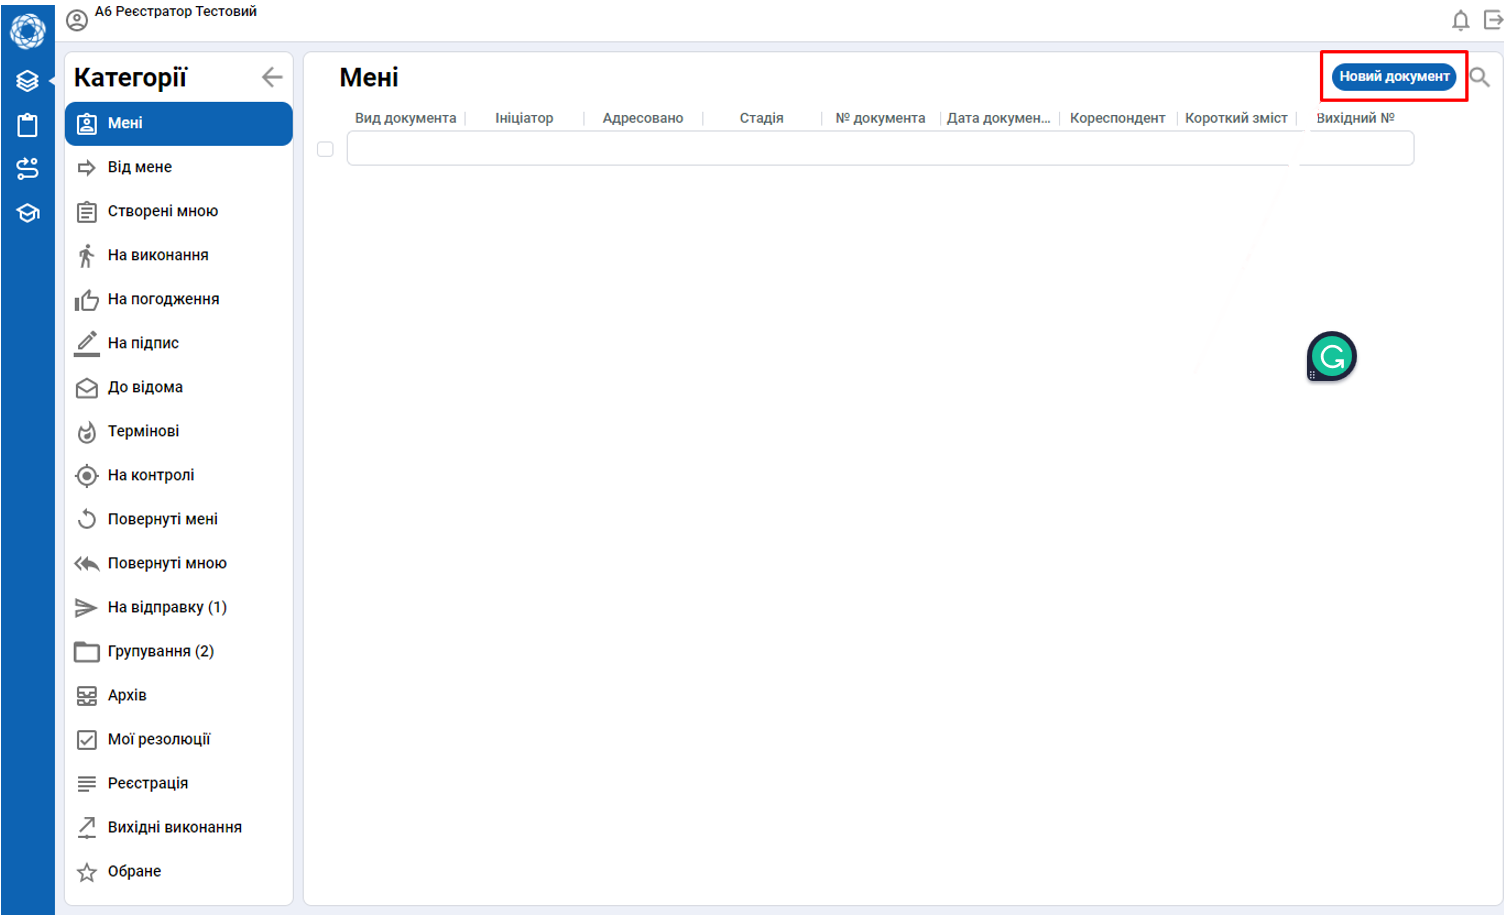
\includegraphics[width=\textwidth]{img/5.1.1.1.png}}
\caption{Рис. 5.1.1.1. Створення нового документа}
\end{figure}

--- Оберіть вид документа з переліку --- Вхідний документ (див. Рисунок 5.1.1.2)

\begin{figure}[!htbp]
\centerline{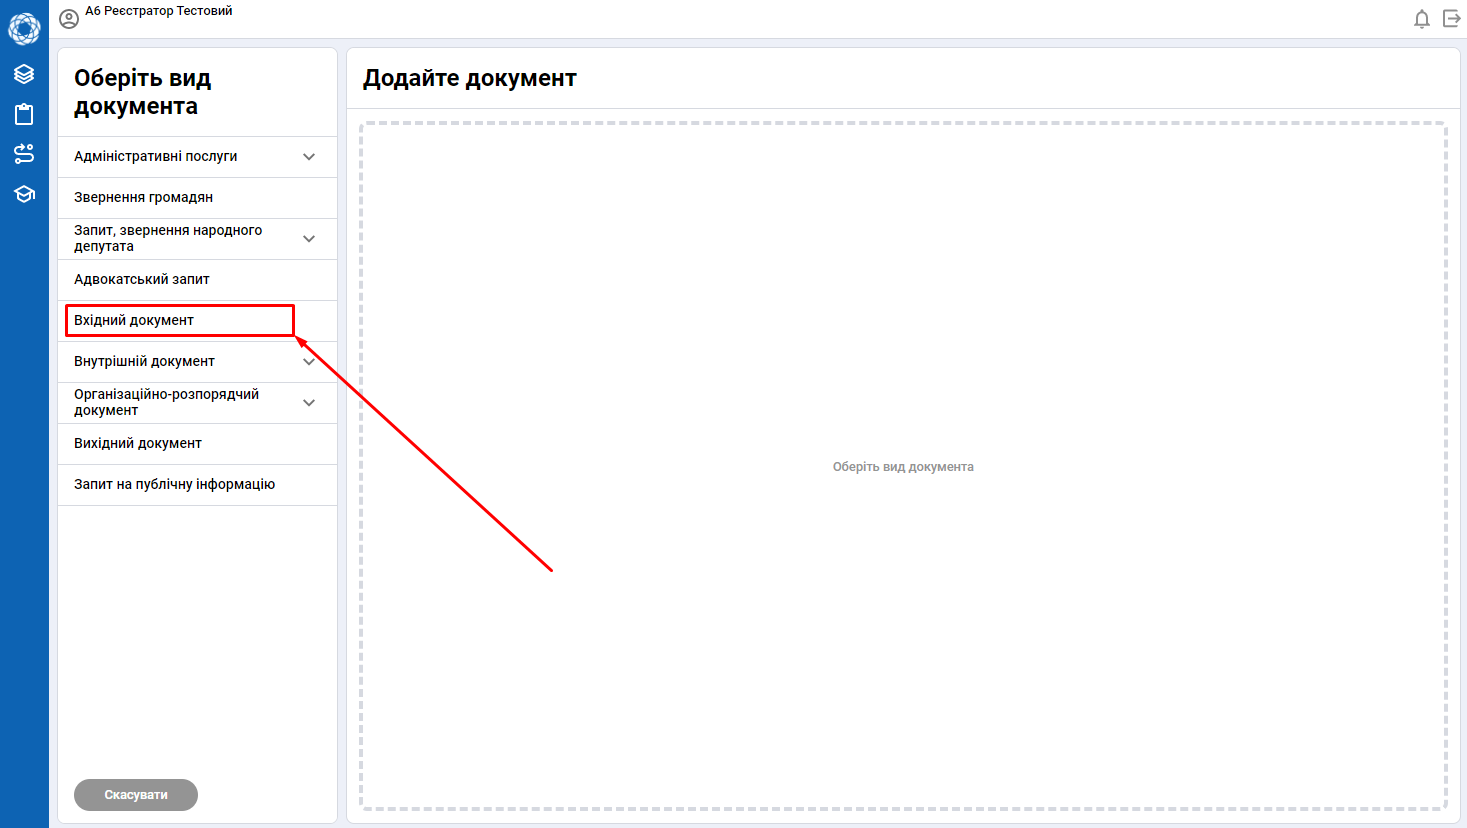
\includegraphics[width=\textwidth]{img/5.1.1.2.png}}
\caption{Рис. 5.1.1.2. Вибір виду документа}
\end{figure}

--- Заповніть РМК (область введення інформації позначена цифрою \circled{3} на
Рисунку 5.1.1.3 \circled{$\ast$} --- поле обов'язкове для заповнення)

\begin{figure}[!htbp]
\centerline{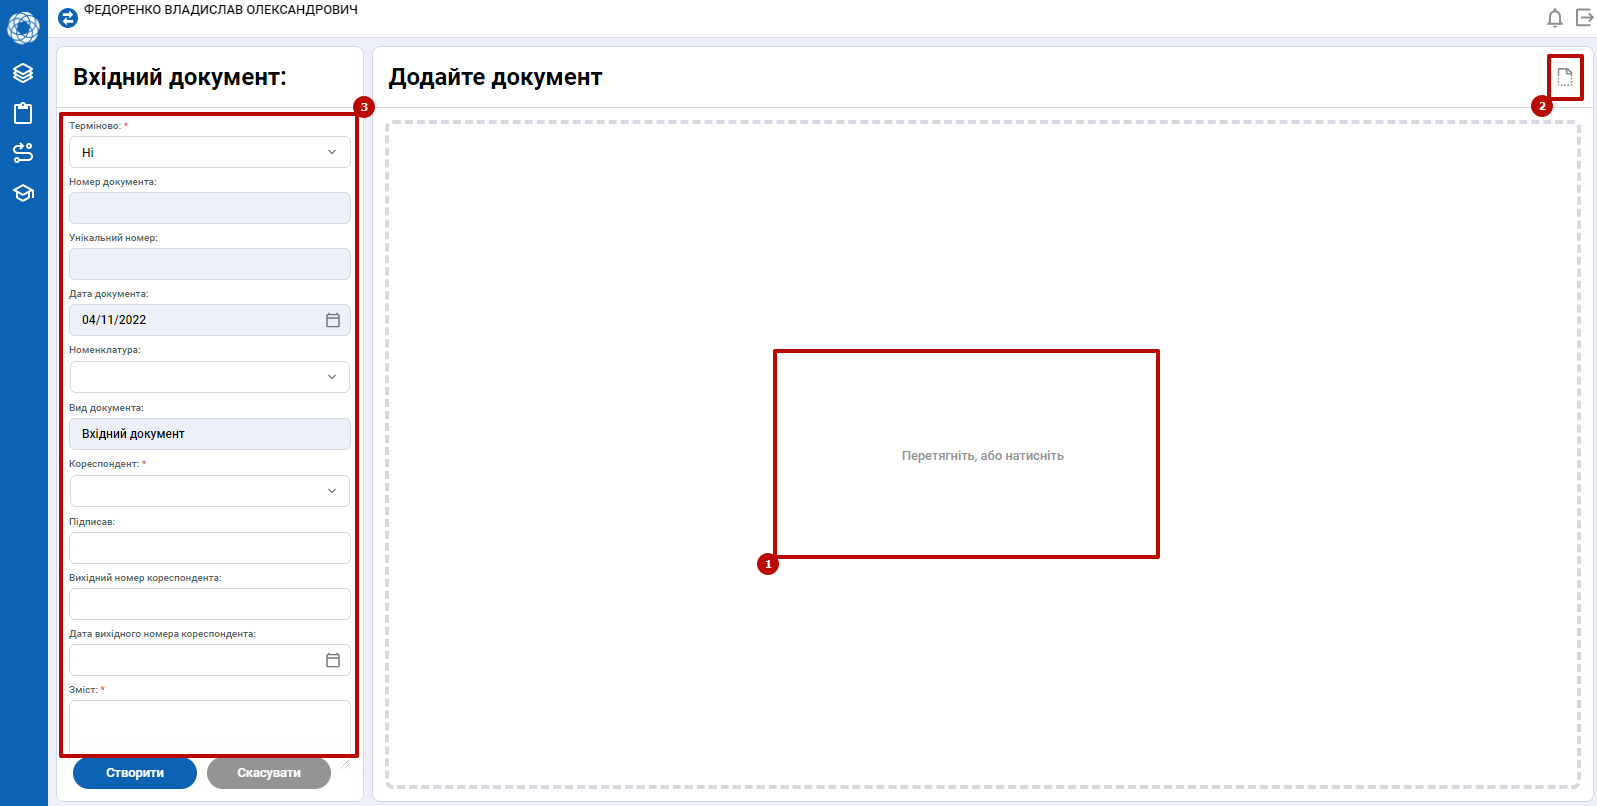
\includegraphics[width=\textwidth]{img/5.1.1.3.png}}
\caption{Рис. 5.1.1.3. Створення РМК}
\end{figure}

--- Додайте файл вхідного документа у зручний для Вас спосіб:
1) активний елемент «Перетягніть, або натисніть», позначений цифрою 1 на Рисунку 5.1.1.3;
2) шляхом сканування $\rightarrow$ піктограма 2 «Сканувати» у правому куті екранної форми (див. Рисунку 5.1.1.3).

\subsection{Сканування}

Для Сканування документа:

--- натисніть піктограму «Сканувати» → відкриється інтерфейс для процесу
сканування (див. Рисунку 5.1.2.1);

--- оберіть необхідний сканер з переліку → позначено цифрою \circled{1};

--- оберіть якість → позначено цифрою \circled{2};

--- за необхідності відредагуйте, використовуючи панель інструментів →
область редагування позначена цифрою \circled{3} в лівій частині екранної форми;

--- оберіть ім'я файлу → позначено цифрою \circled{4};

--- збережіть документ → позначено цифрою \circled{5}.

\begin{figure}[!htbp]
\centerline{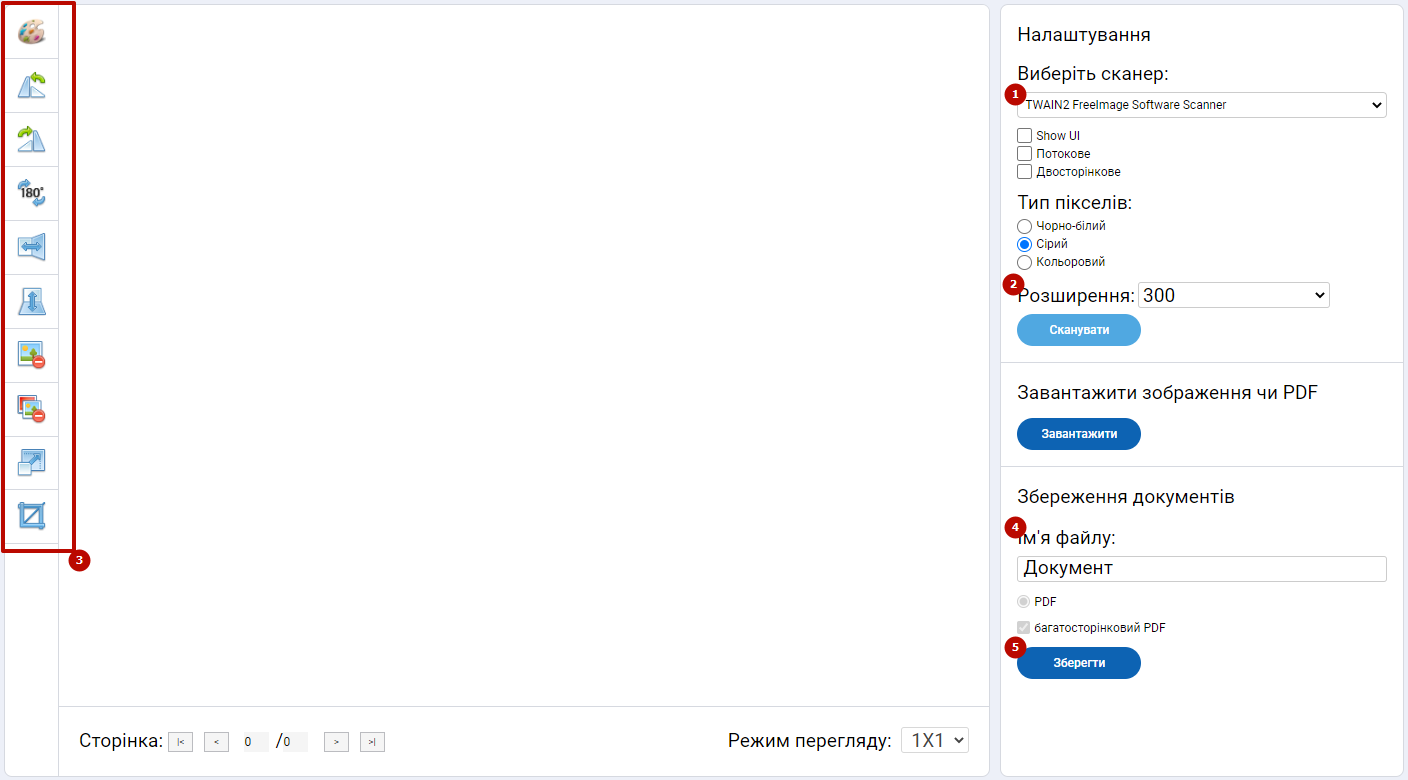
\includegraphics[width=\textwidth]{img/5.1.2.1.png}}
\caption{Рис. 5.1.2.1. Процес сканування}
\end{figure}

Доданий документ на екрані буде виглядати так, як зображено на Рисунку 5.1.2.2:

--- щоб виділити основний документ від його додатків → натисніть кнопку «Зробити основним», позначено цифрою \circled{1};

--- щоб закінчити процес створення документа → натисніть активний елемент «Створити», позначено цифрою \circled{2}.

\begin{figure}[!htbp]
\centerline{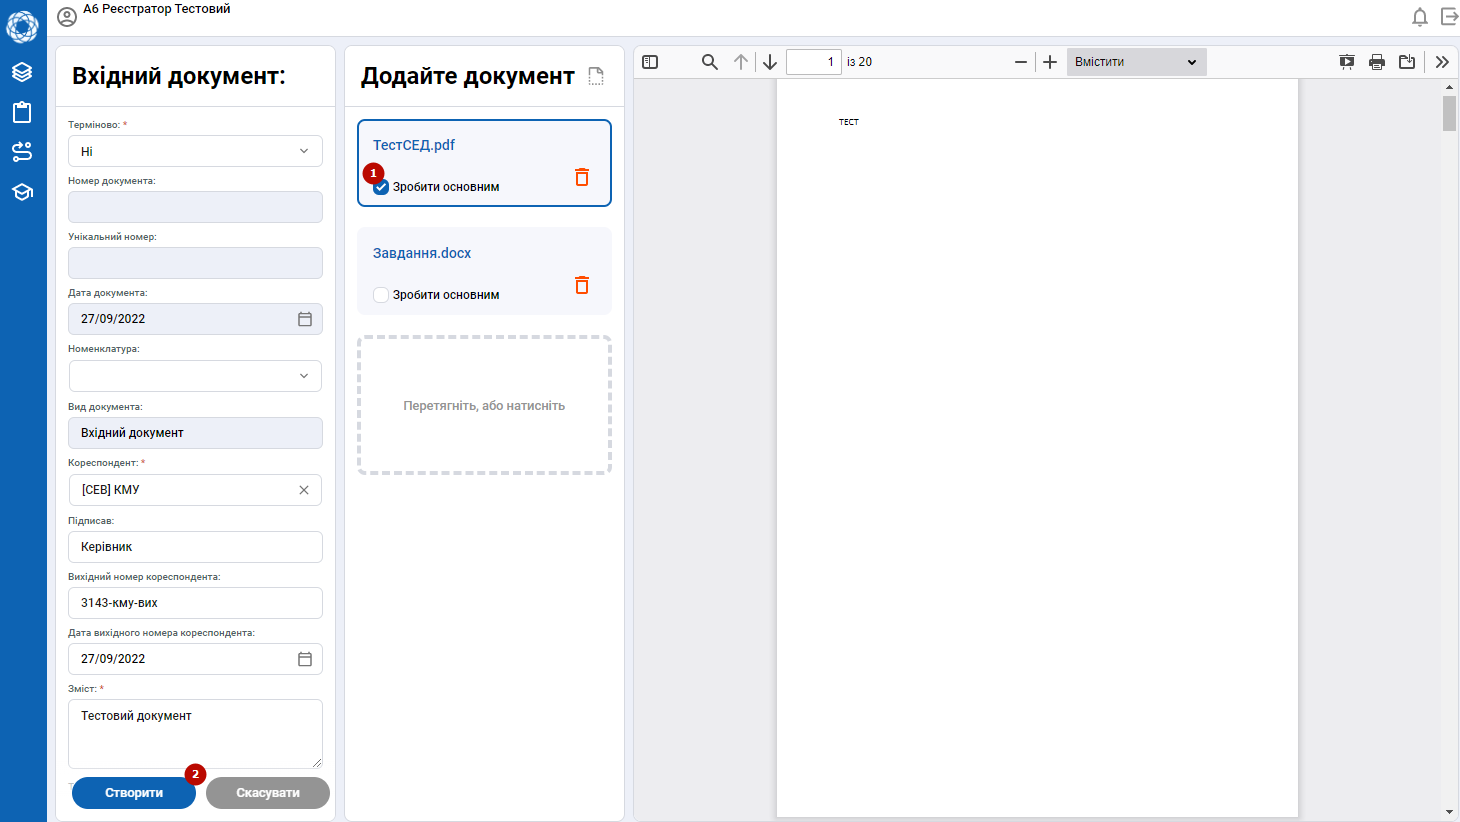
\includegraphics[width=\textwidth]{img/5.1.2.2.png}}
\caption{Рис. 5.1.2.2. Процес створення документа}
\end{figure}

\subsection{Редагування}

Для Редагування реєстраційно-моніторингової картки:

--- натисніть на піктограму із зображенням олівця у правому верхньому куті
лівої частини екранної форми, позначено цифрою \circled{1} на Рисунку 5.1.3.1;

\begin{figure}[!htbp]
\centerline{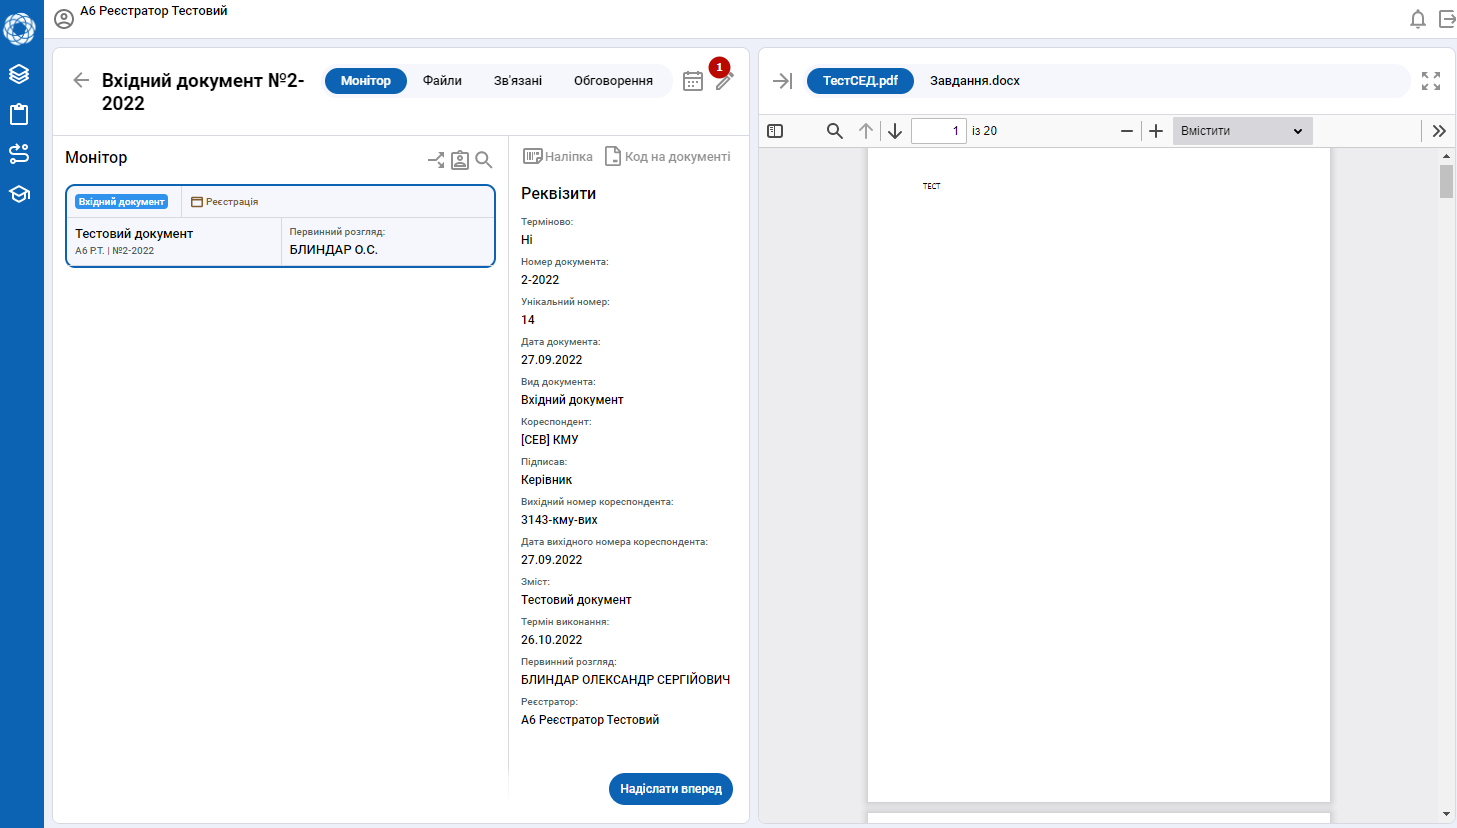
\includegraphics[width=\textwidth]{img/5.1.3.1.png}}
\caption{Рис. 5.1.3.1. Редагування}
\end{figure}

інтерфейс документа видозміниться так, як показано на Рисунку 5.1.3.2;
--- для внесення змін в документ скористайтеся активними елементами,
позначені цифрами на Рисунку 5.1.3.2: \circled{1} --- область для внесення змін реквізитів;
\circled{2} --- активний елемент, що розкриває додаткове меню, де можна додавати/
видаляти документи (див. Рисунку 5.1.3.3 підменю позначено цифрою 2.1);
\circled{3} --- можливість сканування документів.

\begin{figure}[!htbp]
\centerline{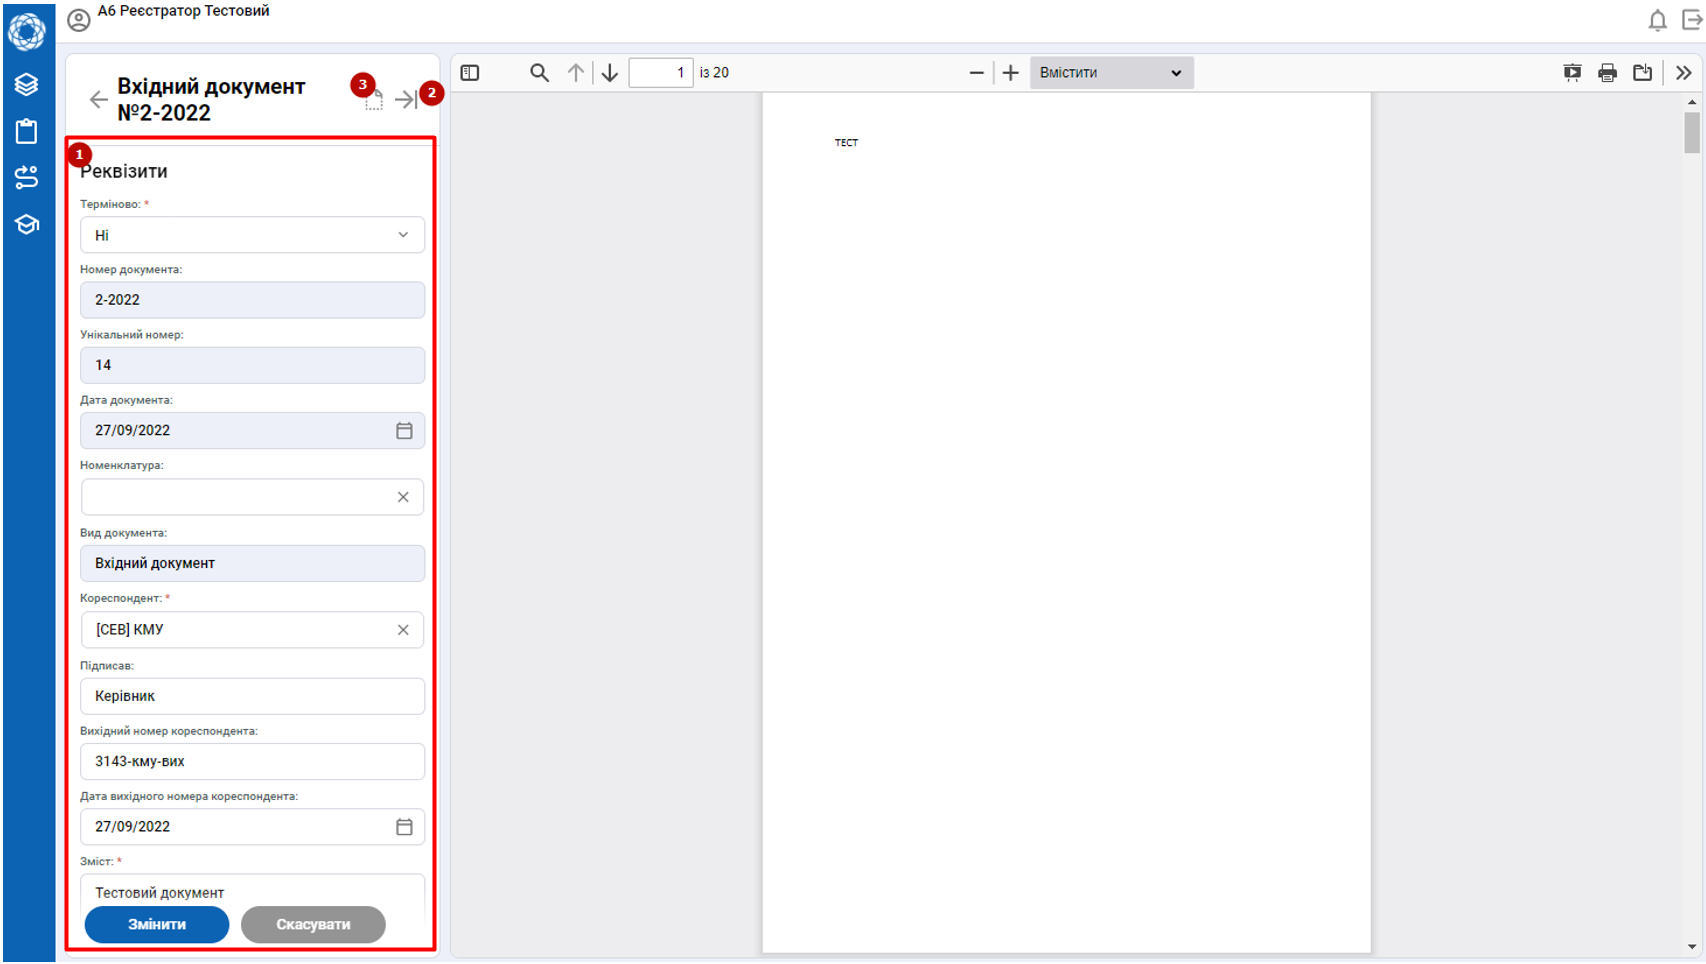
\includegraphics[width=\textwidth]{img/5.1.3.2.png}}
\caption{Рис. 5.1.3.2. Процес редагування документа}
\end{figure}

щоб додати/ видалити документ → скористайтеся активним елементом
позначеним цифрою 2 на Рисунку 5.1.3.2 → у розкритому підменю 2.1 (див.
Рисунку 5.1.3.3) виконайте необхідні дії;

--- щоб закріпити зміни → натисніть «Змінити» позначено цифрою \circled{1} або
«Скасувати» позначено цифрою \circled{2} на Рисунку 5.1.3.3.

\begin{figure}[!htbp]
\centerline{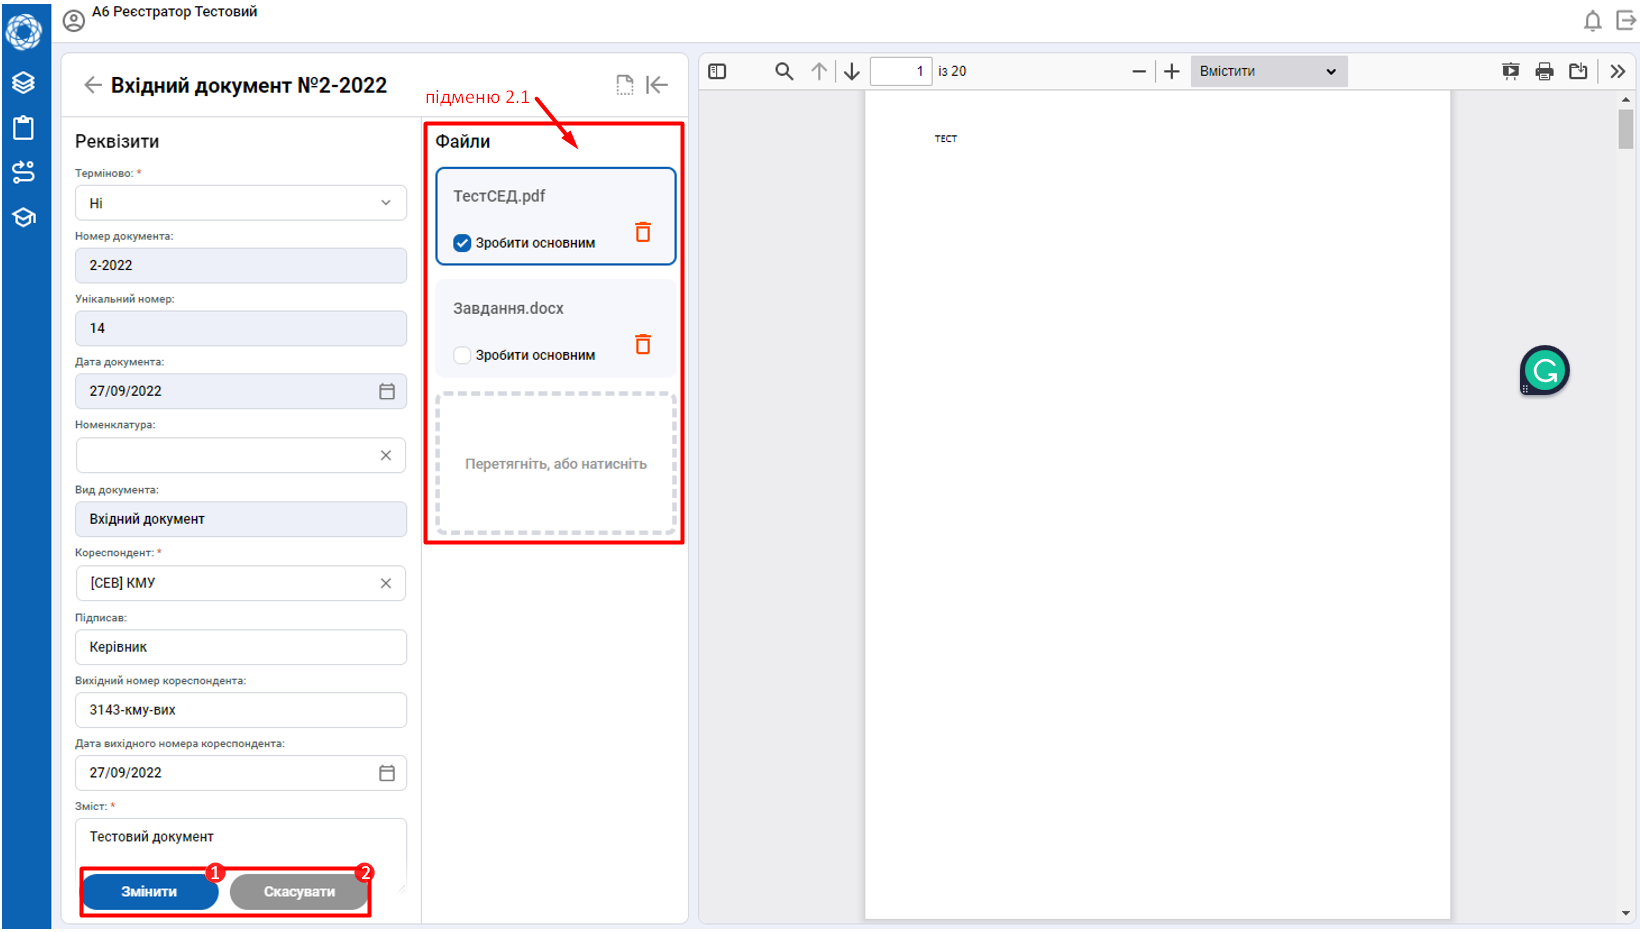
\includegraphics[width=\textwidth]{img/5.1.3.3.png}}
\caption{Рис. 5.1.3.3. Закінчення редагування документа}
\end{figure}

Для закінчення процесу Реєстрації документа:
--- натисніть активний елемент «Надіслати вперед» → позначено цифрою \circled{1} на Рисунку 5.1.3.4;
--- такі дії можливі в разі визначення особи первинного розгляду → позначено рамкою на Рисунку 5.1.3.4;

\begin{figure}[!htbp]
\centerline{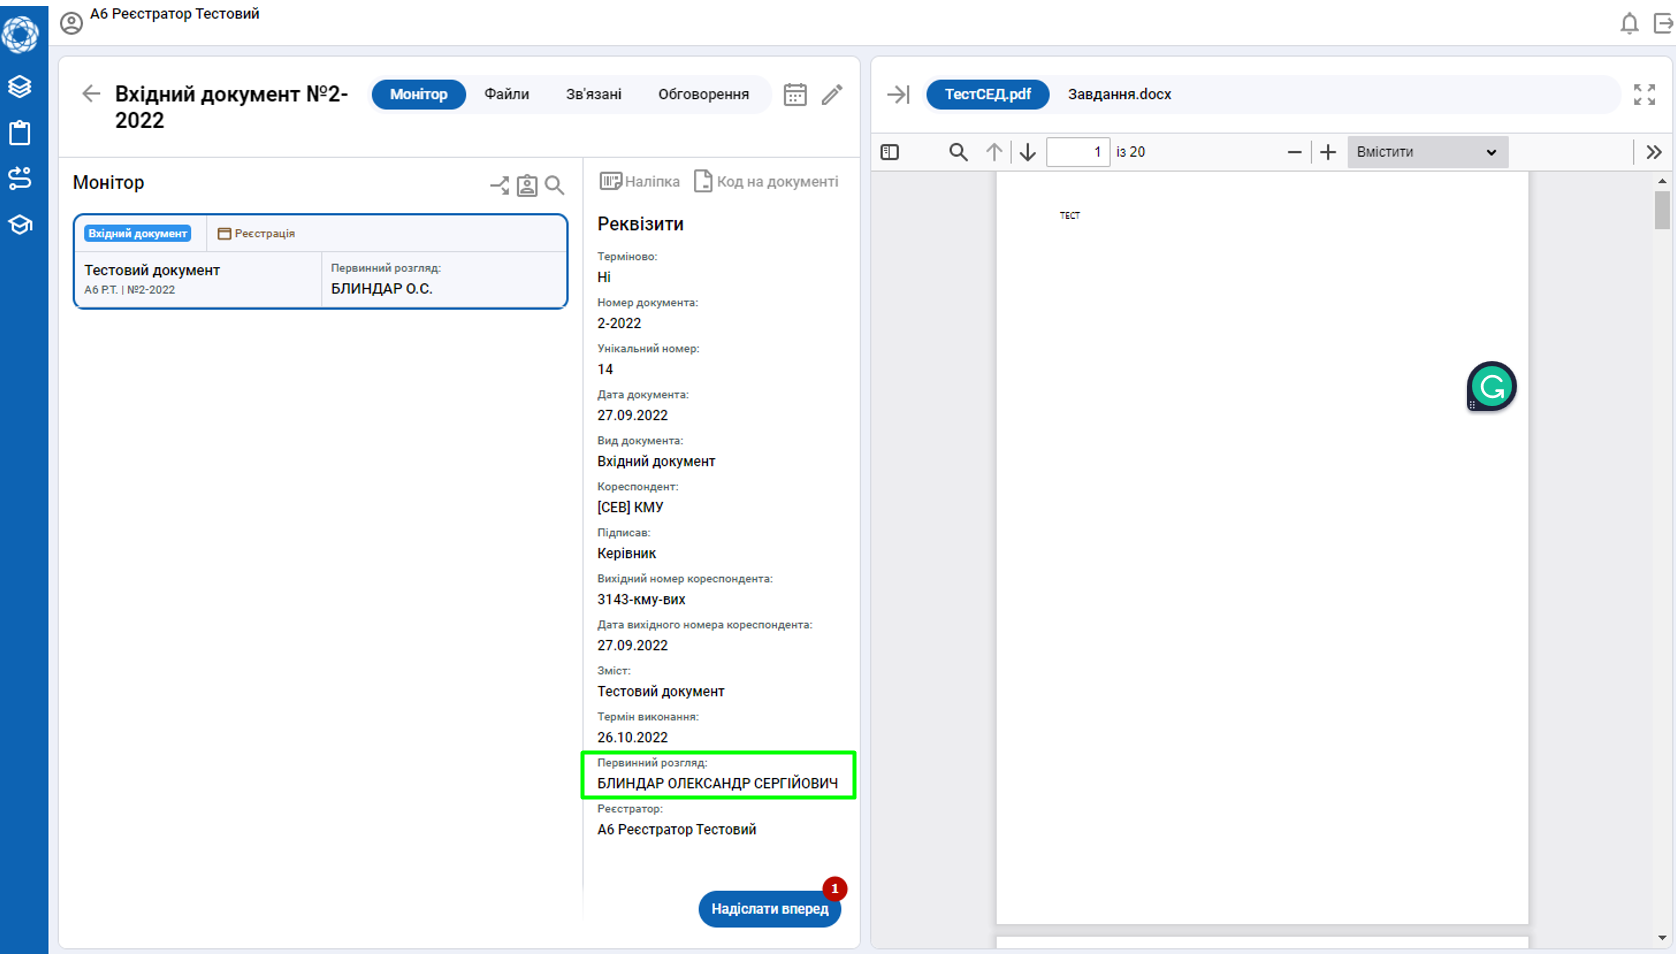
\includegraphics[width=\textwidth]{img/5.1.3.4.png}}
\caption{Рис. 5.1.3.4. Завершальний етап процесу реєстрації документа}
\end{figure}

якщо особа первинного розгляду не вказана → натиснуть активний елемент
«Надіслати вперед» → позначено цифрою \circled{1} на Рисунку 5.1.3.5 → документ
буде скеровано відповідальній особі на стадію «Визначення», яка визначить особу первинного розгляду.
--- Поруч з папкою «На визначення» з'явиться

\begin{figure}[!htbp]
\centerline{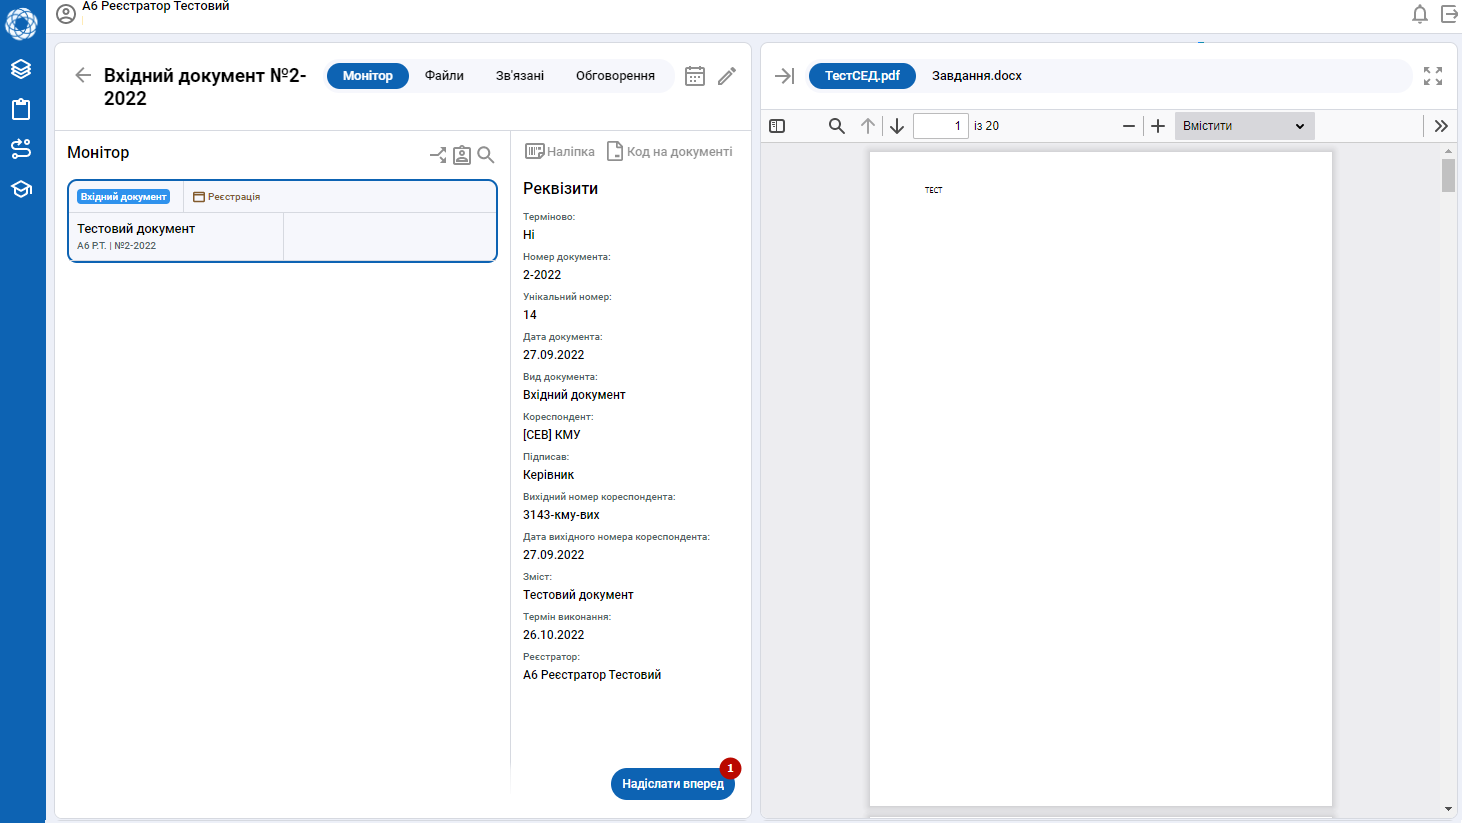
\includegraphics[width=\textwidth]{img/5.1.3.5.png}}
\caption{Рис. 5.1.3.5. Не вказано особу первинного розгляду}
\end{figure}

\subsection{Визначення}

Папка «На визначення» (див. Рисунок 5.1.4.1) містить документи, що потребують
визначення особи або декількох осіб первинного розгляду.
Особу/ осіб первинного розгляду визначає користувач, що має відповідні
повноваження (помічник директора, директор).

\begin{figure}[!htbp]
\centerline{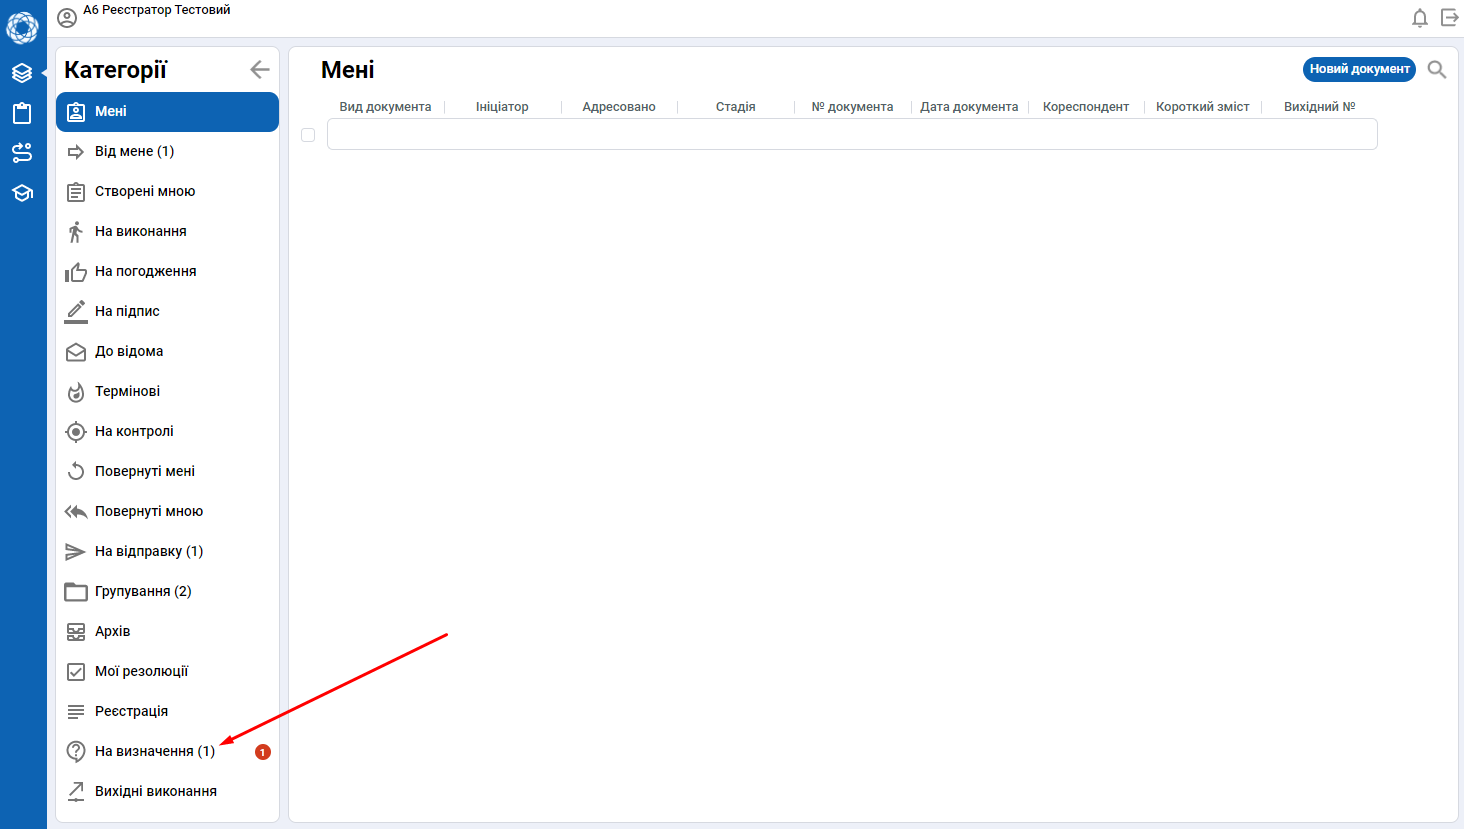
\includegraphics[width=\textwidth]{img/5.1.4.1.png}}
\caption{Рис. 5.1.4.1. Меню робочого столу користувача}
\end{figure}

Для визначення осіб первинного розгляду:
--- відкрийте документ → натисніть на піктограму із зображенням олівця
(Редагування) → позначено цифрою \circled{1} на Рисунку 5.1.4.2;

\begin{figure}[!htbp]
\centerline{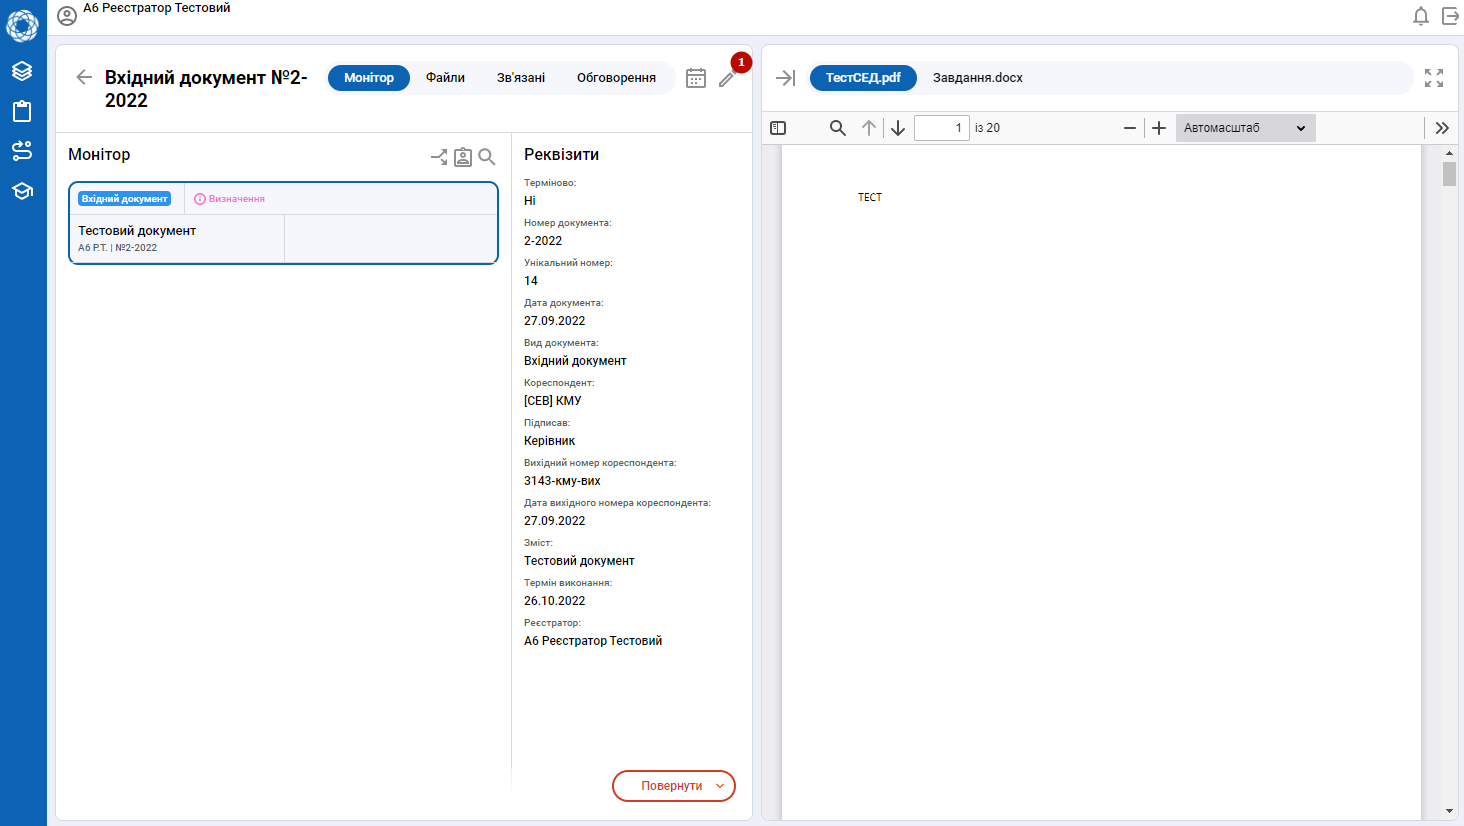
\includegraphics[width=\textwidth]{img/5.1.4.2.png}}
\caption{Рис. 5.1.4.2. }
\end{figure}

заповніть поле «Первинний розгляд» → позначено цифрою \circled{1} на Рисунку 5.1.4.3;
--- щоб підтвердити зміни → натисніть активний елемент «Змінити» → позначено цифрою \circled{2} на Рисунку 5.1.4.3.

\begin{figure}[!htbp]
\centerline{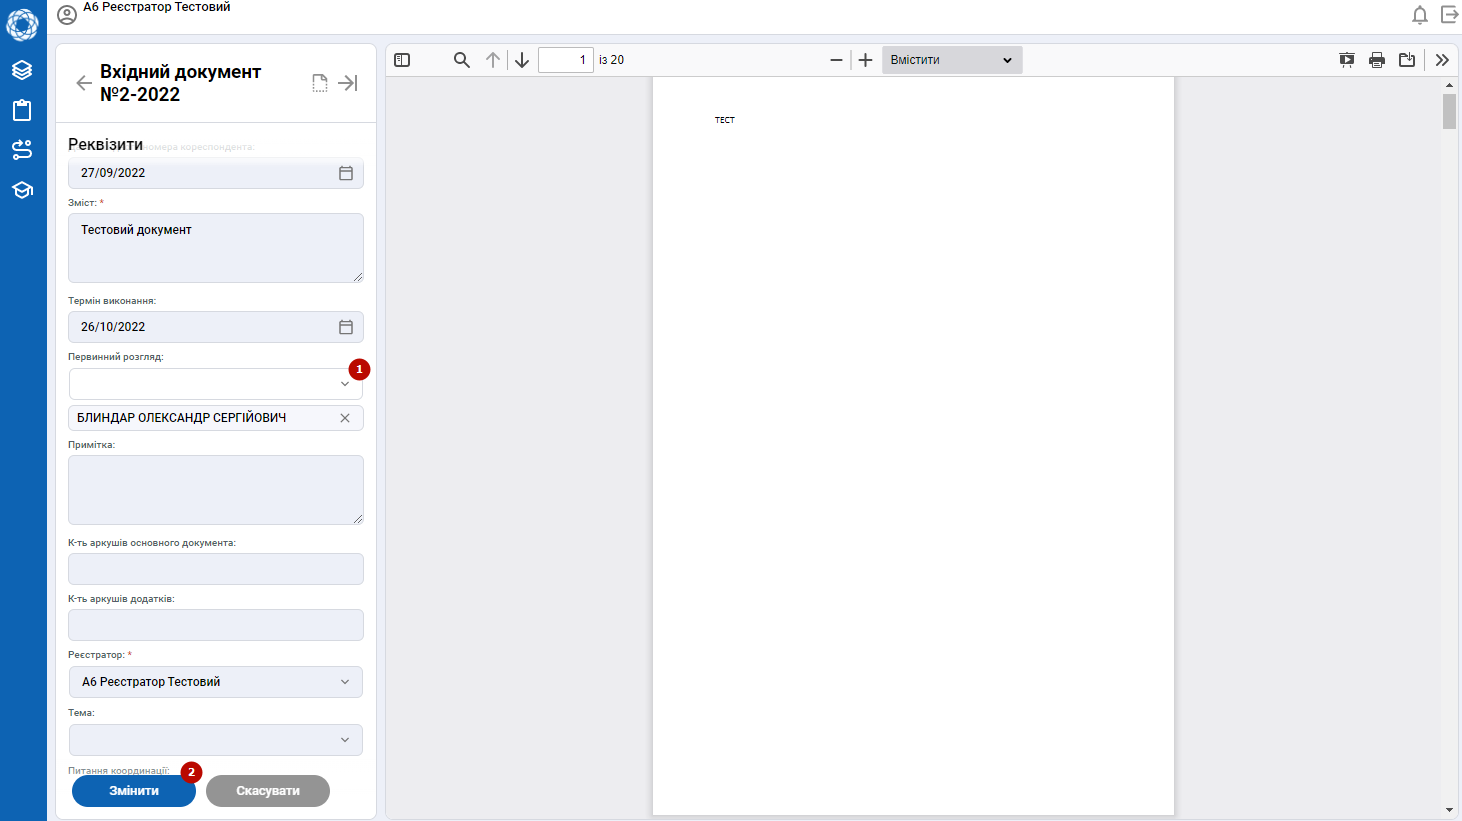
\includegraphics[width=\textwidth]{img/5.1.4.3.png}}
\caption{Рис. 5.1.4.3. }
\end{figure}

щоб завершити процес «Визначення» → натисніть активний елемент «На
первинний розгляд» → позначено цифрою \circled{1} на Рисунку 5.1.4.4.

\begin{figure}[!htbp]
\centerline{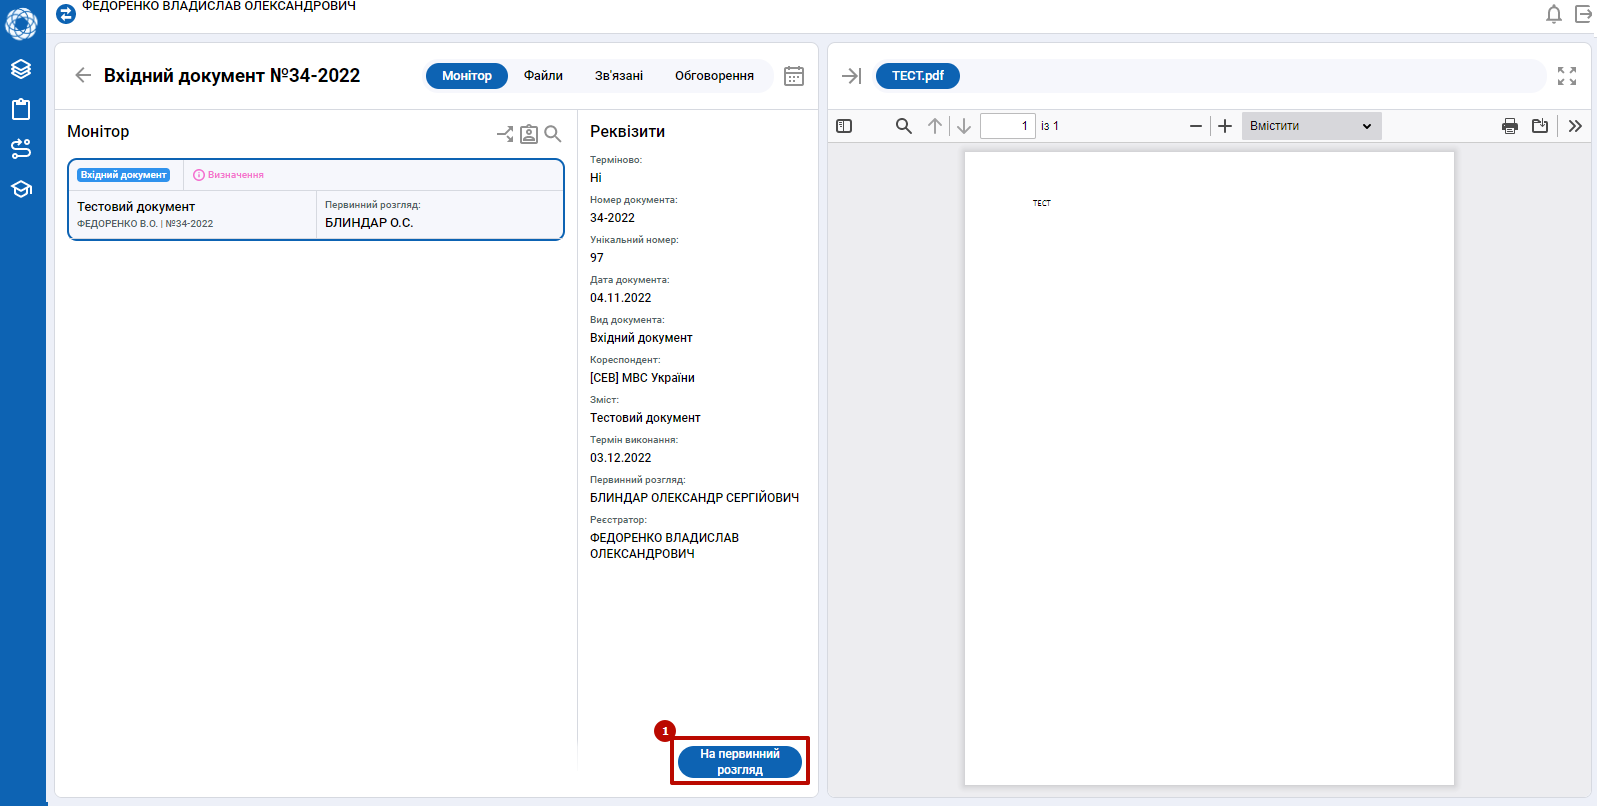
\includegraphics[width=\textwidth]{img/5.1.4.4.png}}
\caption{Рис. 5.1.4.4. }
\end{figure}

\section{Резолюція}

\subsection{Повернення документа на реєстрацію}

Для повернення вхідного документа на Реєстрацію:
--- натисніть активний елемент «Повернути» → позначено цифрою \circled{1} на Рисунку 5.2.1.1;
--- виберіть пункт «На реєстрацію» → позначено цифрою \circled{2}.

\begin{figure}[!htbp]
\centerline{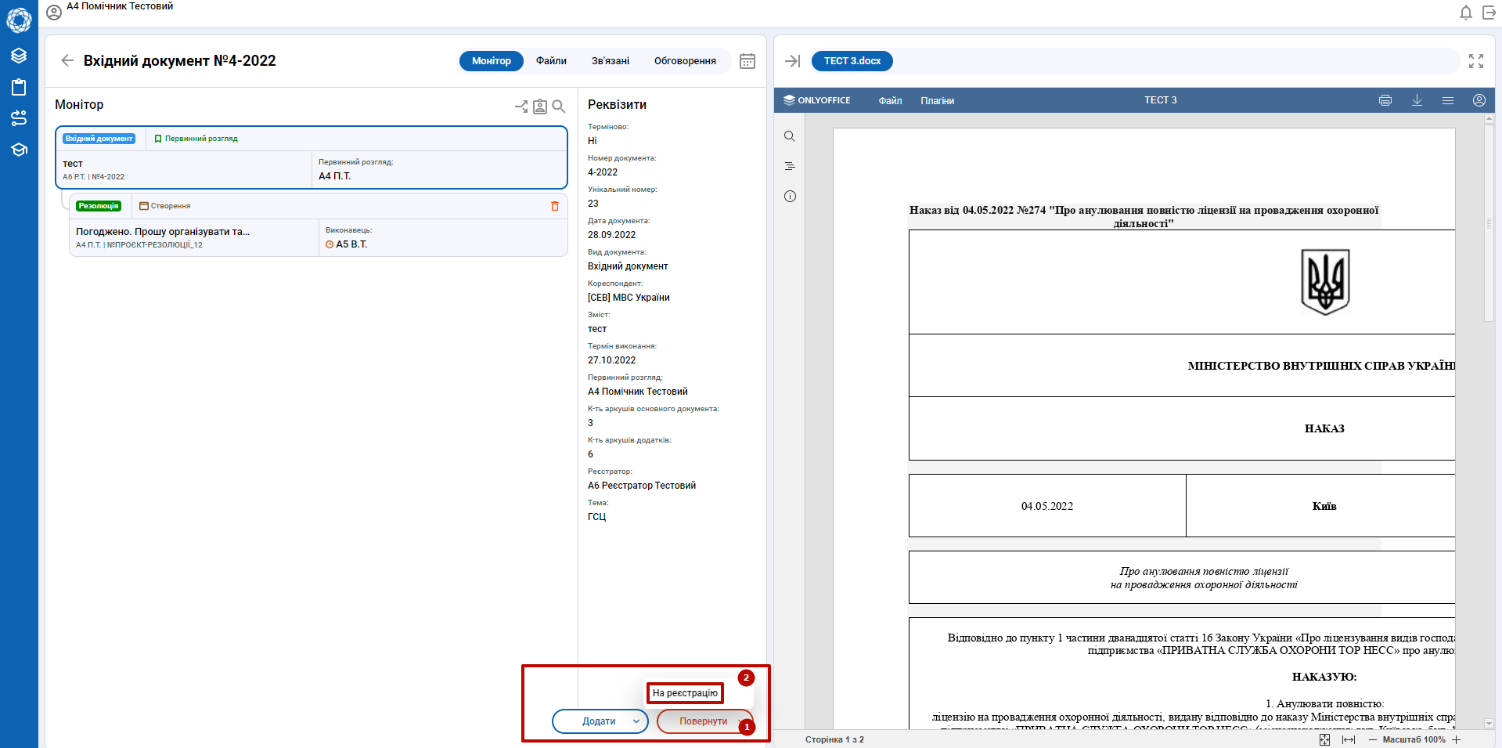
\includegraphics[width=\textwidth]{img/5.2.1.1.png}}
\caption{Рис. 5.2.1.1. }
\end{figure}

--- вкажіть причину повернення → \circled{1} «Змінити особу первинного розгляду» →
натисніть на кнопку, позначену цифрою \circled{2} на Рисунку 5.2.1.2.

\begin{figure}[!htbp]
\centerline{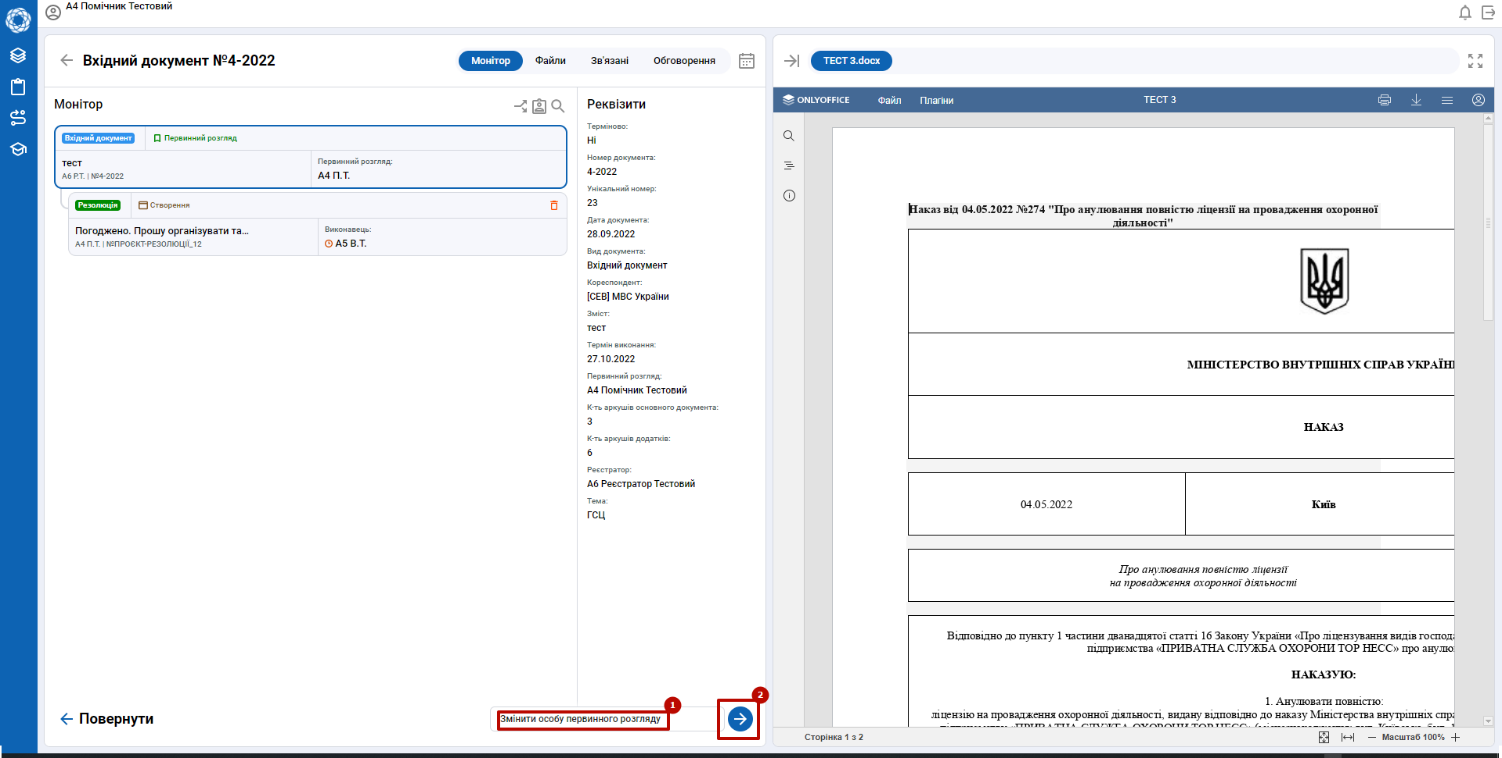
\includegraphics[width=\textwidth]{img/5.2.1.2.png}}
\caption{Рис. 5.2.1.2. Повернення документа на Реєстрацію}
\end{figure}

\subsection{Створення проєкту резолюції}

Для Створення проєкту резолюції помічник/ особа первинного розгляду/ посадова особа, яка отримала резолюцію (завдання):
--- натисніть активний елемент «Додати» → позначено цифрою \circled{1} на Рисунку 5.2.2.1;
--- оберіть пункт «Резолюція» → позначено цифрою \circled{2} на Рисунку 5.2.2.1.

\begin{figure}[!htbp]
\centerline{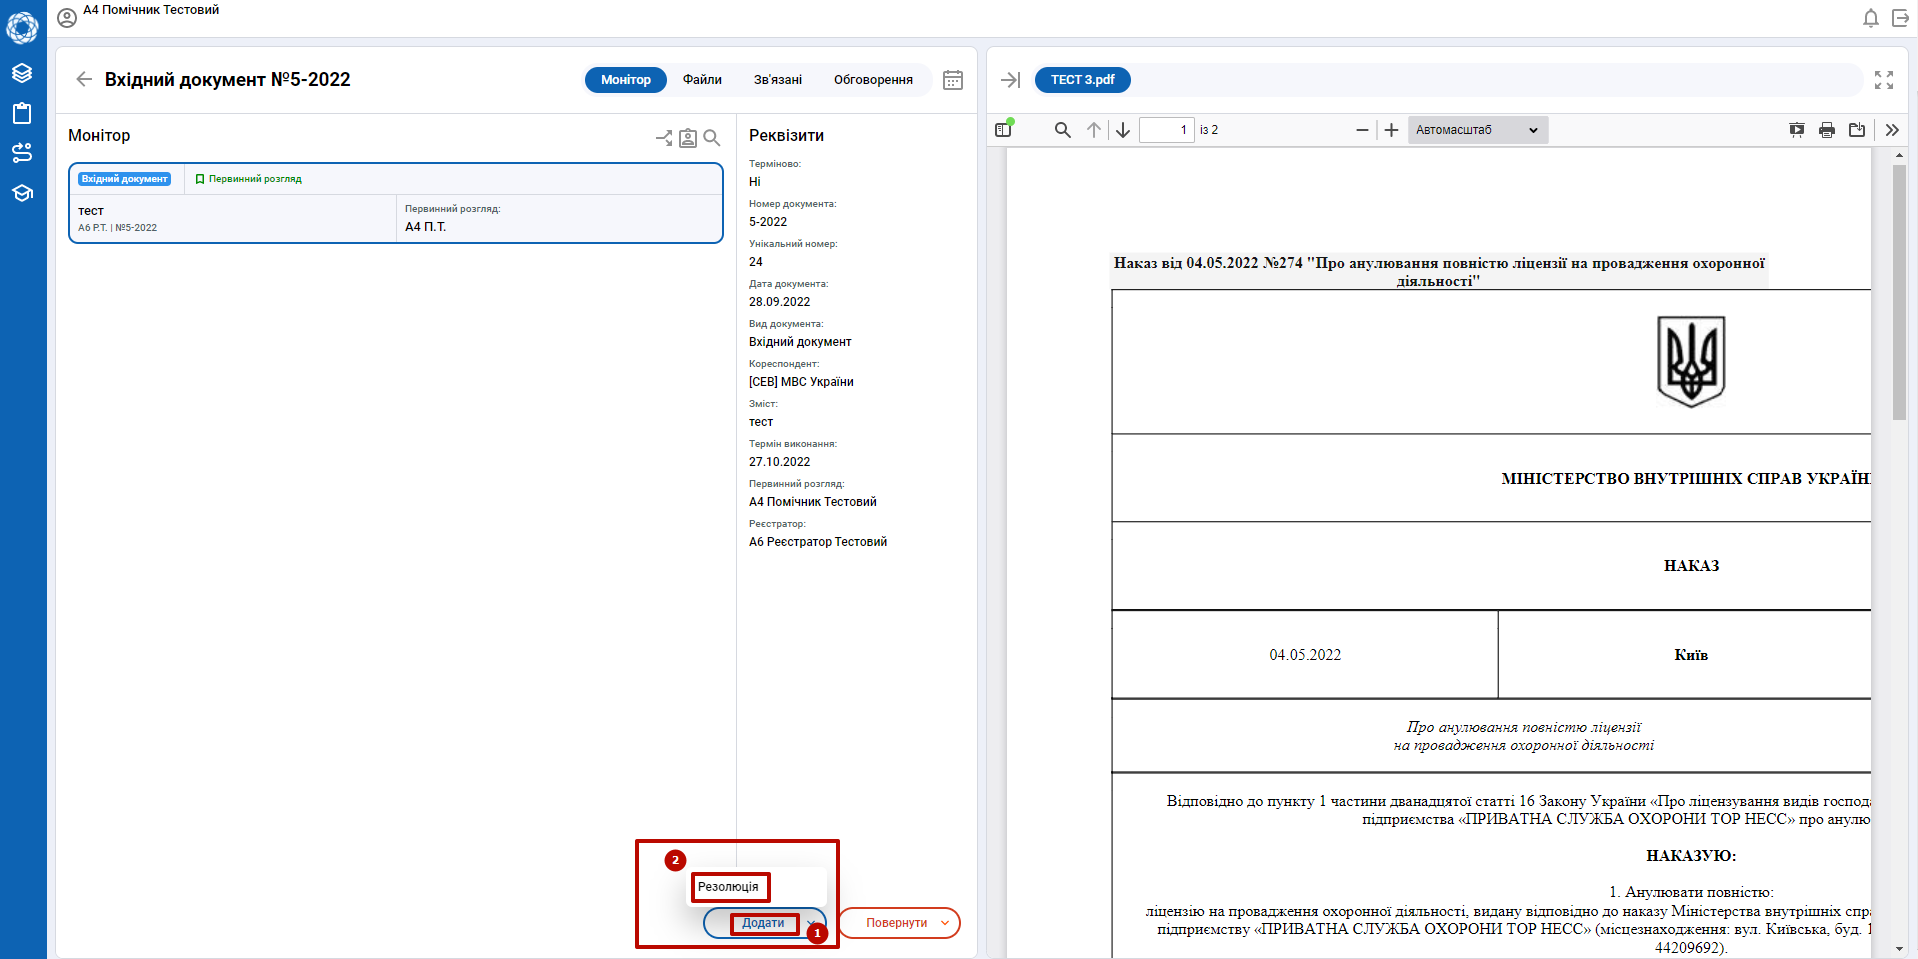
\includegraphics[width=\textwidth]{img/5.2.2.1.png}}
\caption{Рис. 5.2.2.1.}
\end{figure}

введіть реквізити проєкта резолюції в область внесення даних → позначено цифрою \circled{1}
на Рисунку 5.2.2.2 → поля відмічені \circled{$\ast$} – обов'язкові для заповнення;
--- щоб підтвердити → натисніть активний елемент «Створити» → позначено цифрою \circled{2}.

\begin{figure}[!htbp]
\centerline{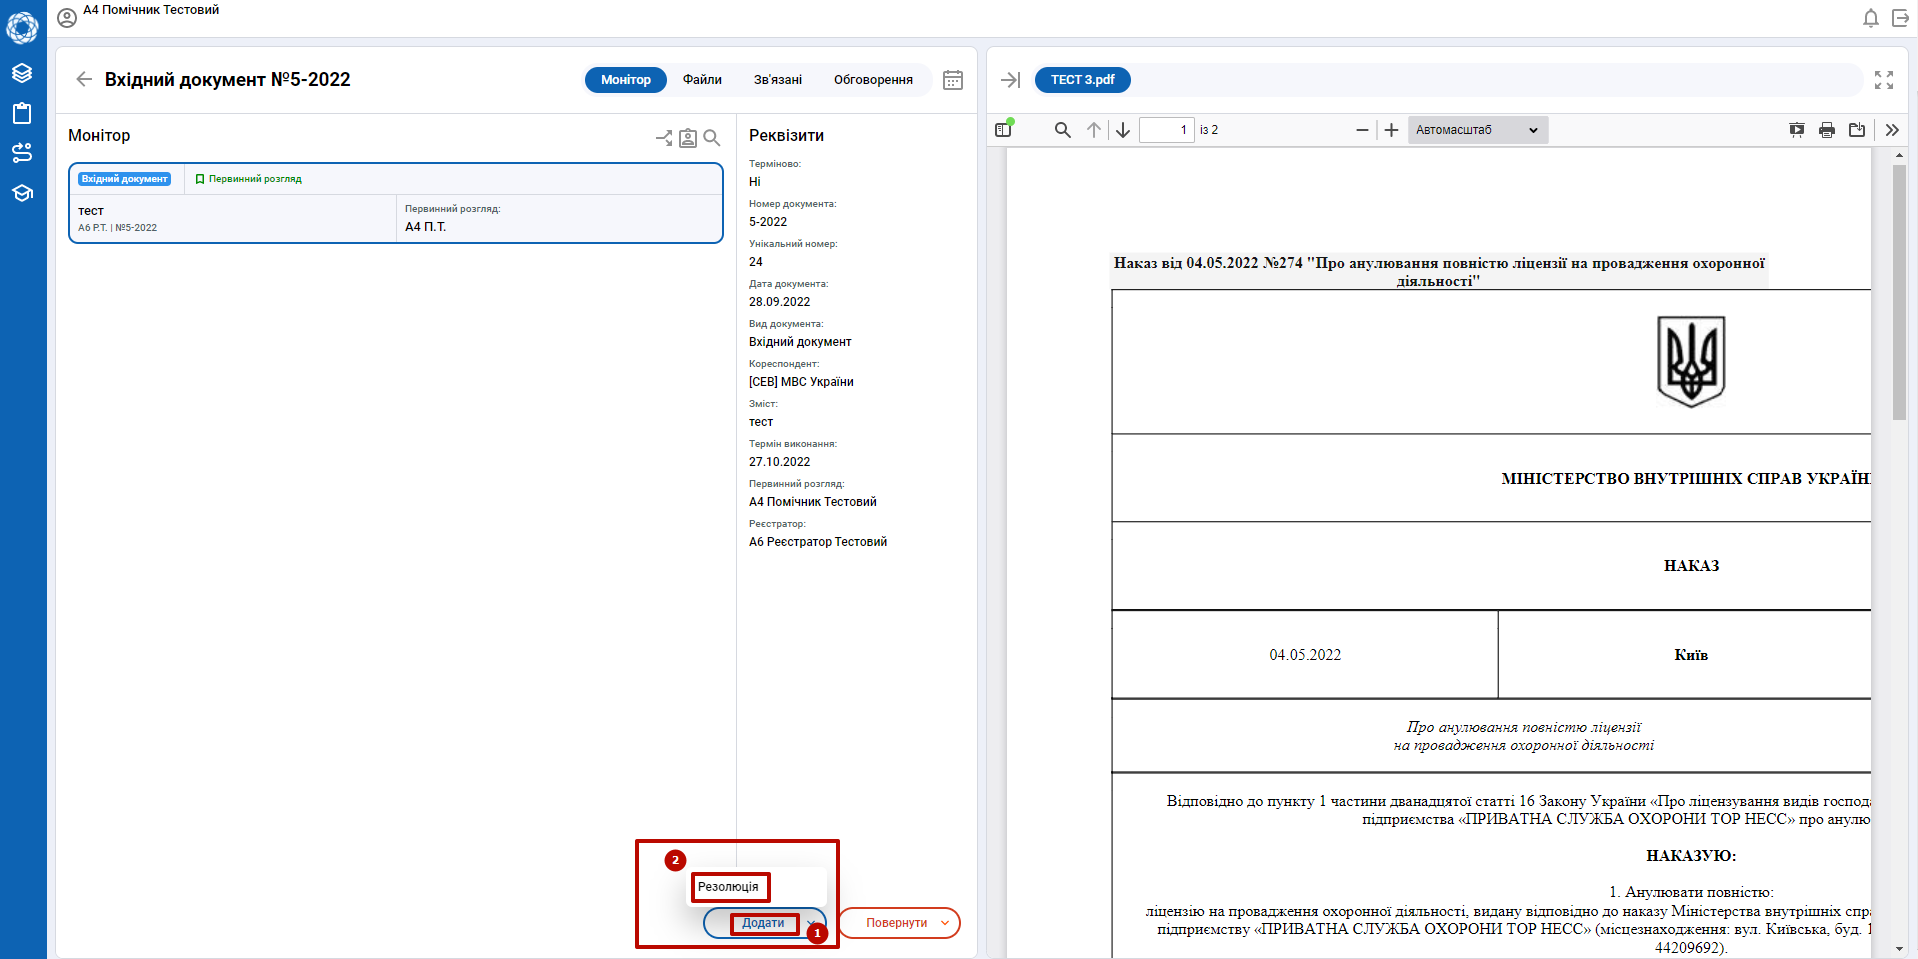
\includegraphics[width=\textwidth]{img/5.2.2.1.png}}
\caption{Рис. 5.2.2.2. Створення проєкту резолюції}
\end{figure}

\subsection{Редагування/видалення проєкту резолюції}

Для Внесення змін у проєкт резолюції:
--- натисніть на піктограму «Редагування» → позначено цифрою \circled{1} на Рисунку 5.2.3.1.

\begin{figure}[!htbp]
\centerline{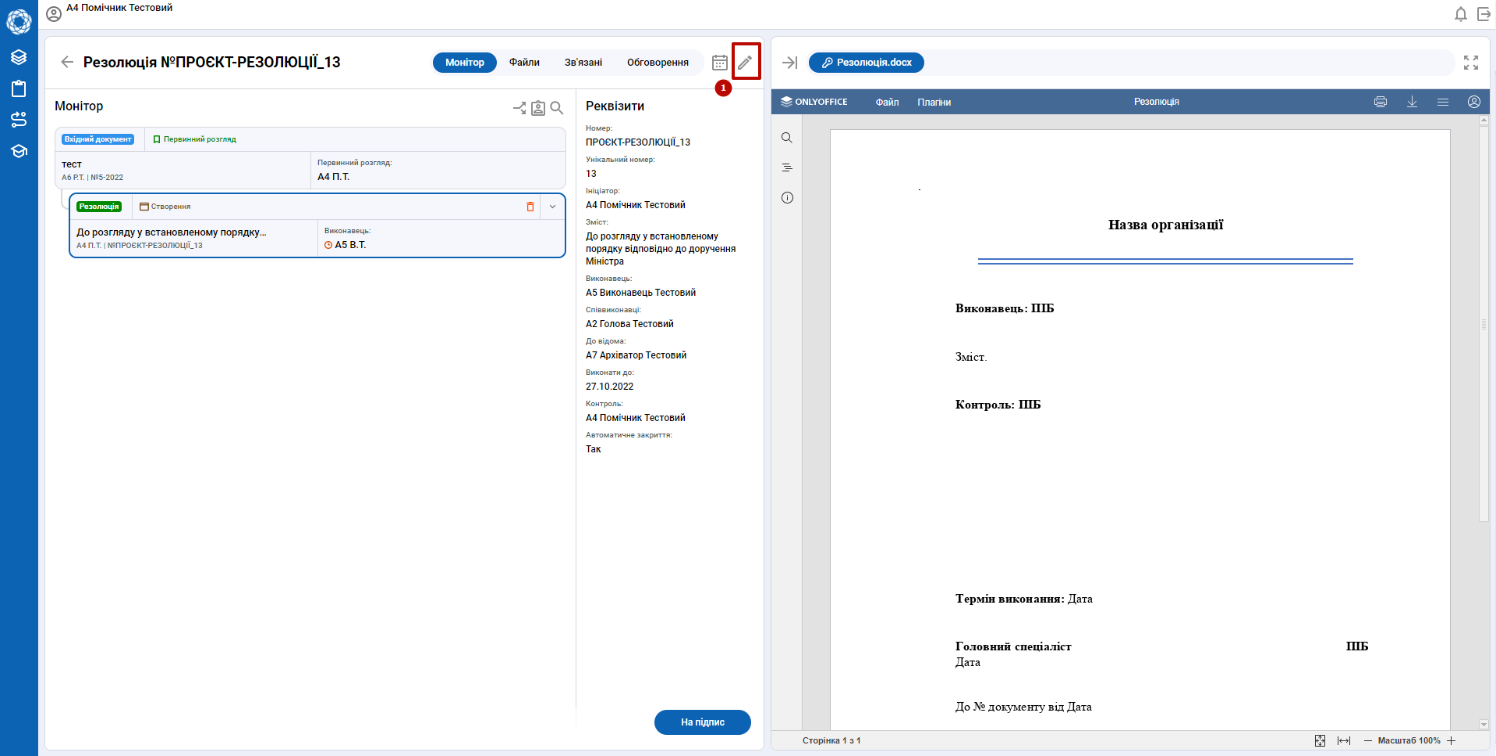
\includegraphics[width=\textwidth]{img/5.2.3.1.png}}
\caption{Рис. 5.2.3.1.}
\end{figure}

--- внесіть необхідні зміни у реквізити документа → для збереження змін
натисніть активний елемент «Змінити» → позначено цифрою \circled{1} на Рисунку 5.2.3.2.

\begin{figure}[!htbp]
\centerline{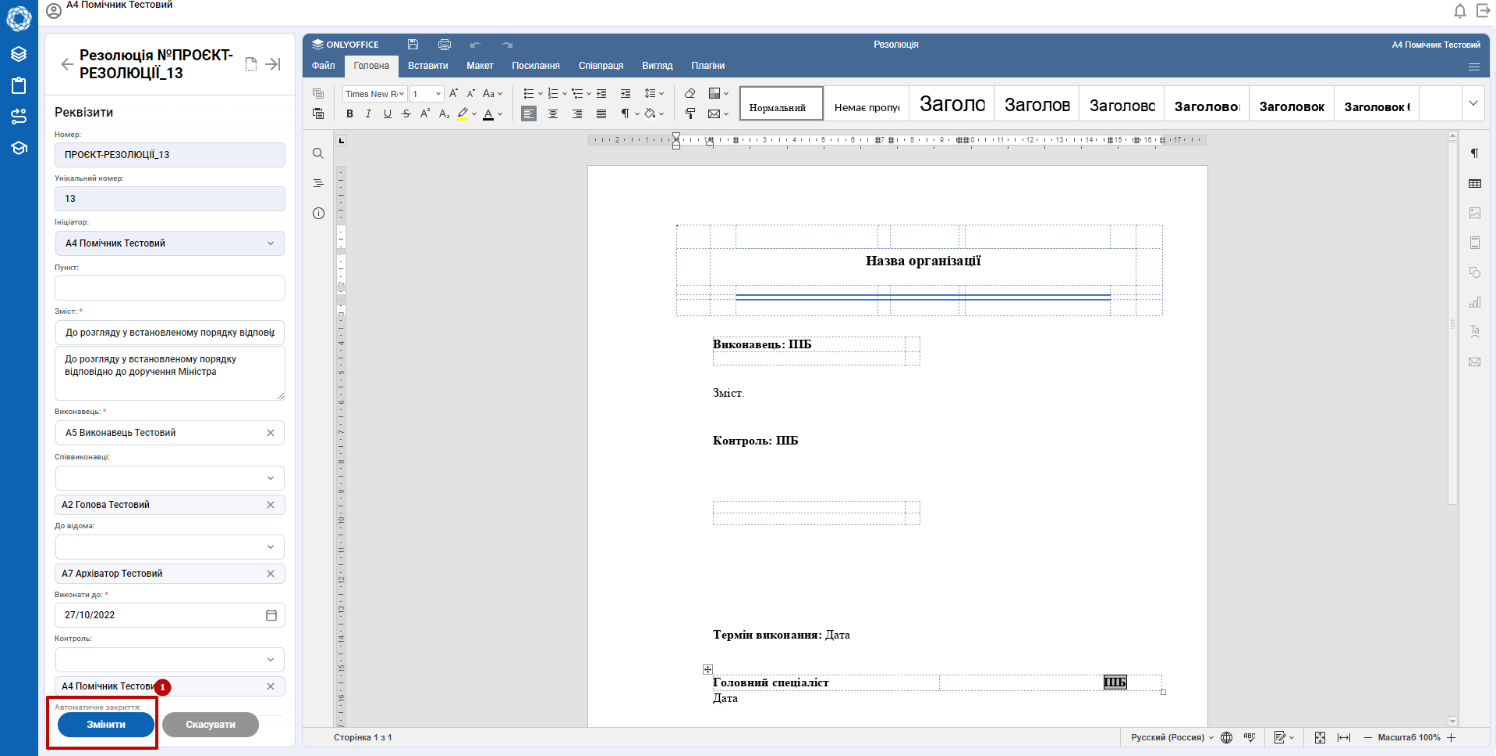
\includegraphics[width=\textwidth]{img/5.2.3.2.png}}
\caption{Рис. 5.2.3.2. Редагування проєкту резолюції}
\end{figure}

Для видалення проєкту резолюції:
--- натисніть піктограму «Видалити» → позначено цифрою \circled{1} на Рисунку 5.2.3.3;
--- розпочніть процес створення резолюції спочатку.

\begin{figure}[!htbp]
\centerline{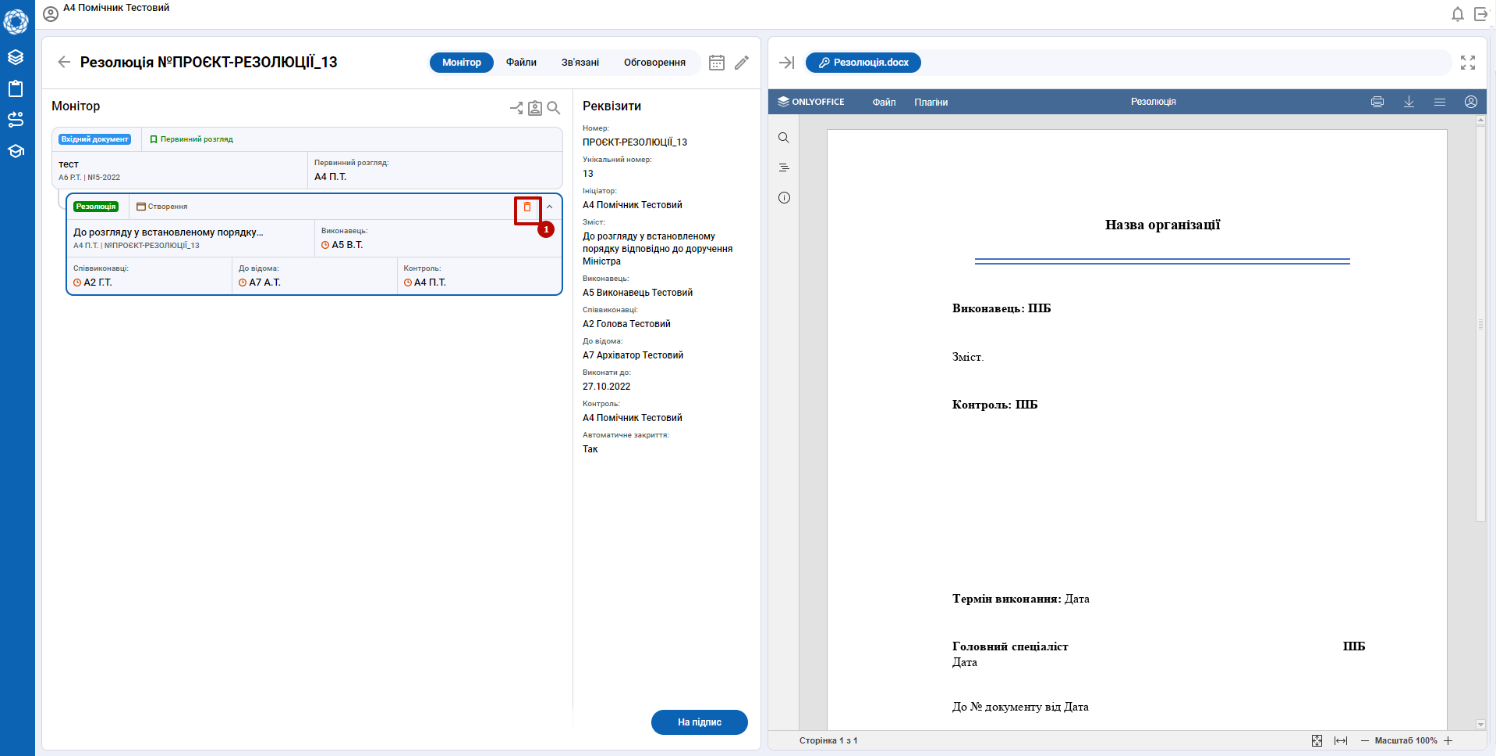
\includegraphics[width=\textwidth]{img/5.2.3.3.png}}
\caption{Рис. 5.2.3.3. Видалення проєкту резолюції}
\end{figure}

\subsection{Підписання проєкту резолюції}

Для Відправлення проєкту резолюції на підписання:
--- натисніть активний елемент «На підпис» → позначено цифрою \circled{1} на Рисунку 5.2.4.1.
--- функція налаштована і доступна керівнику, якому підготовлено проєкт резолюції,
помічнику та особі, що формує проєкт резолюції без помічника.

\begin{figure}[!htbp]
\centerline{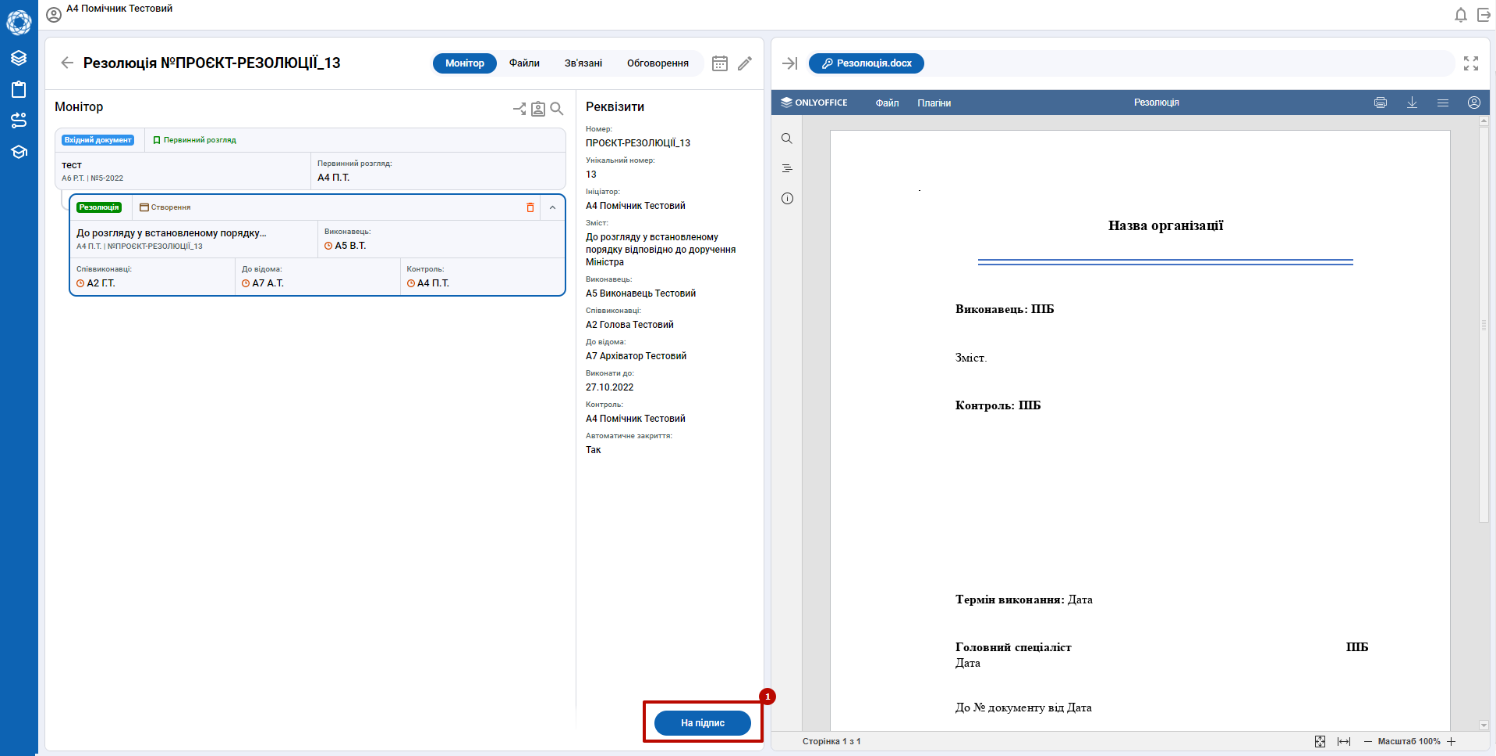
\includegraphics[width=\textwidth]{img/5.2.4.1.png}}
\caption{Рис. 5.2.4.1. }
\end{figure}

Для підпису проєкту резолюції:
--- натисніть активний елемент «Підписати» → позначено цифрою \circled{1} на Рисунку 5.2.4.2.
Для повернення проєкту резолюції на Створення:
--- натисніть активний елемент «Повернути» → позначено цифрою \circled{2} →
виберіть пункт «На створення» → позначено цифрою \circled{3} на Рисунку 5.2.4.2.

\begin{figure}[!htbp]
\centerline{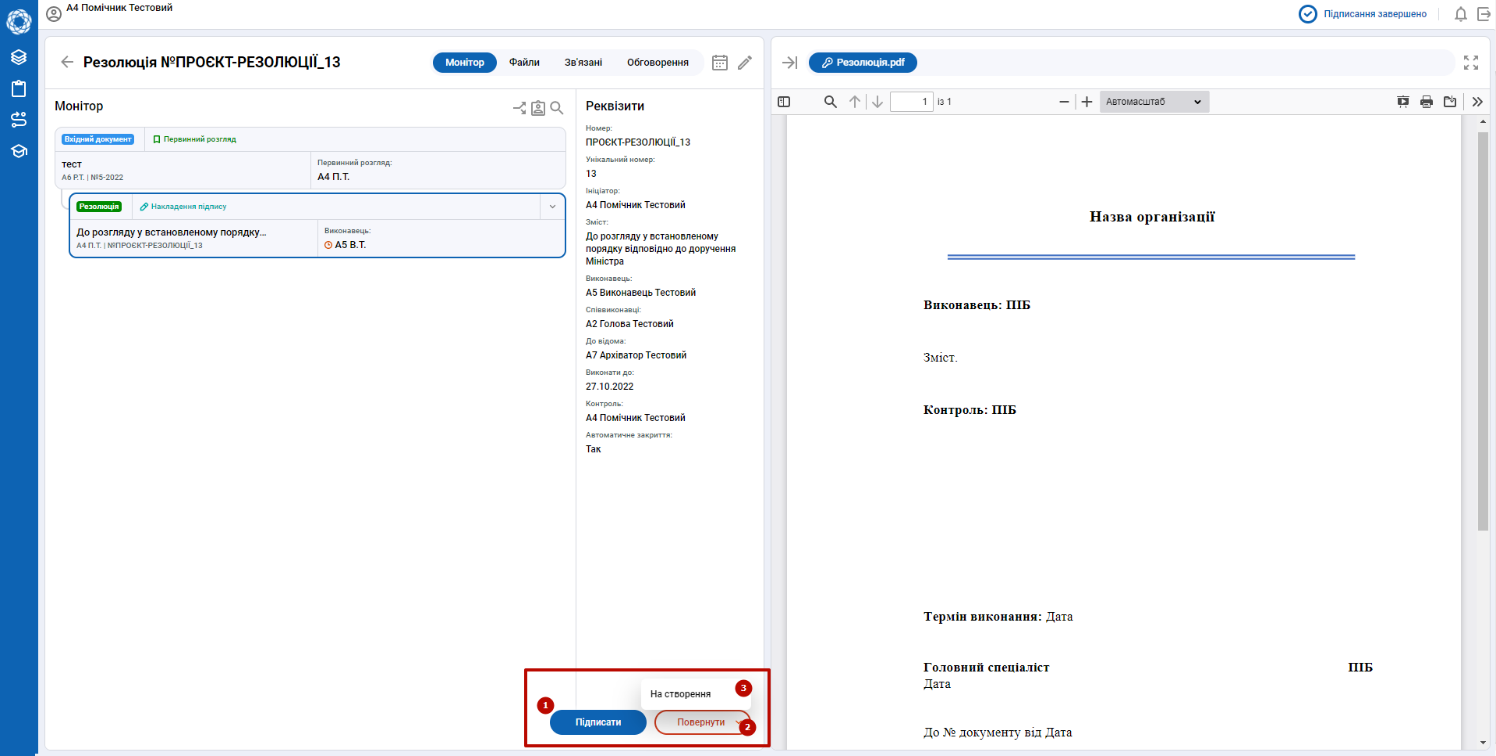
\includegraphics[width=\textwidth]{img/5.2.4.2.png}}
\caption{Рис. 5.2.4.2. }
\end{figure}

\subsection{Виконання/відхилення резолюції}

Резолюція стосовно виконання вхідного документа може передбачати проведення
виконавцем певних дій (підготувати документ) або бути нейтральною, наприклад
«взято до відома». В усіх випадках необхідно підтвердити Виконання:
--- натисніть активний елемент «Виконано» → позначено цифрою \circled{1} на Рисунку 5.2.5.1;
--- обов'язково зазначте результат опрацювання на вкладці «Обговорення» →
позначено цифрою \circled{2} на Рисунку 5.2.5.1.

\section{Вихідний документ}

\begin{figure}[!htbp]
\centerline{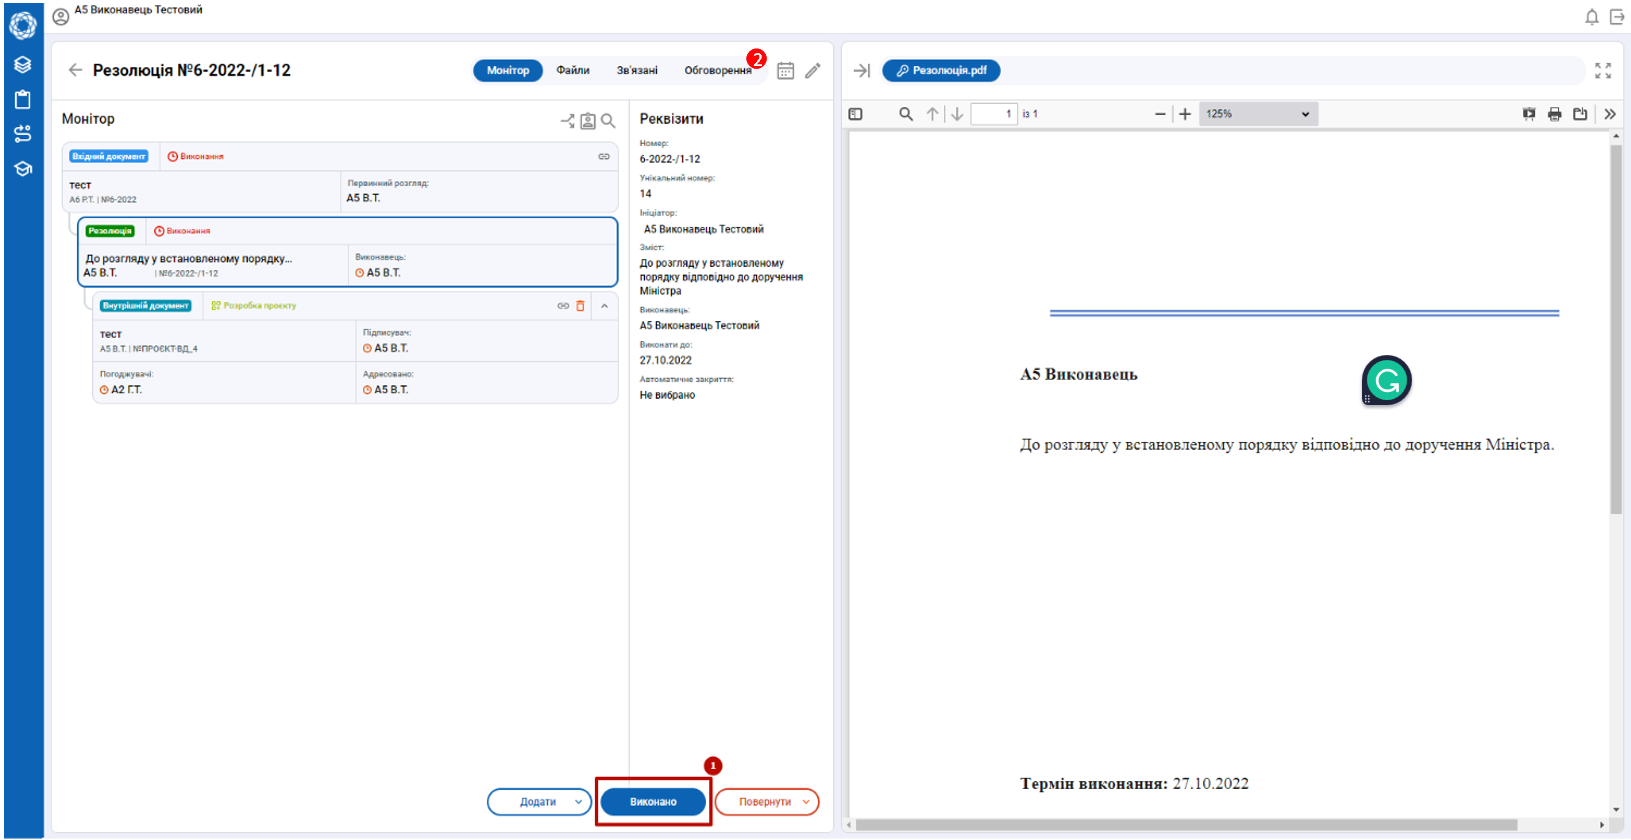
\includegraphics[width=\textwidth]{img/5.2.5.1.png}}
\caption{Рис. 5.2.5.1. Підтвердження виконання листа}
\end{figure}

щоб скористатися підменю вкладки «Обговорення» → натисніть на цю
вкладку, що позначена цифрою \circled{2} на Рисунку 5.2.5.1 → з'явиться нова
форма екранного меню, що містить поля для введення інформації та
коментарів → як це показано на Рисунку 5.2.5.2.

Цифрами на Рисунку 5.2.5.2 позначено:
\circled{1} --- поточна вкладка;
\circled{2} --- поле для введення тесту з вказанням результату опрацювання документа;
\circled{3} --- поле для коментарів.

\begin{figure}[!htbp]
\centerline{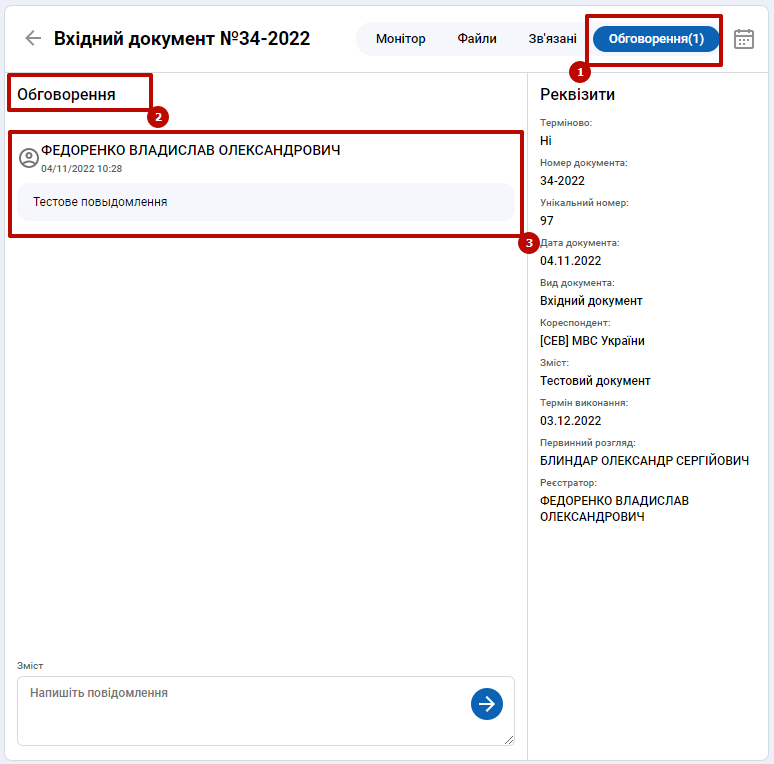
\includegraphics[width=\textwidth]{img/5.2.5.2.png}}
\caption{Рис. 5.2.5.2. Результат опрацювання документа}
\end{figure}

В процесі розгляду вхідного документа виконавцем, може з'ясуватися, що
призначене завдання знаходиться поза межами його компетенції, у такому разі
документ повертають на попередню стадію:
--- натисніть активний елемент «Повернути» → позначено цифрою \circled{1} на Рисунку 5.2.5.3;
--- обрати пункт «На попередню стадію» → позначено цифрою \circled{2} на Рисунку 5.2.5.3.

\begin{figure}[!htbp]
\centerline{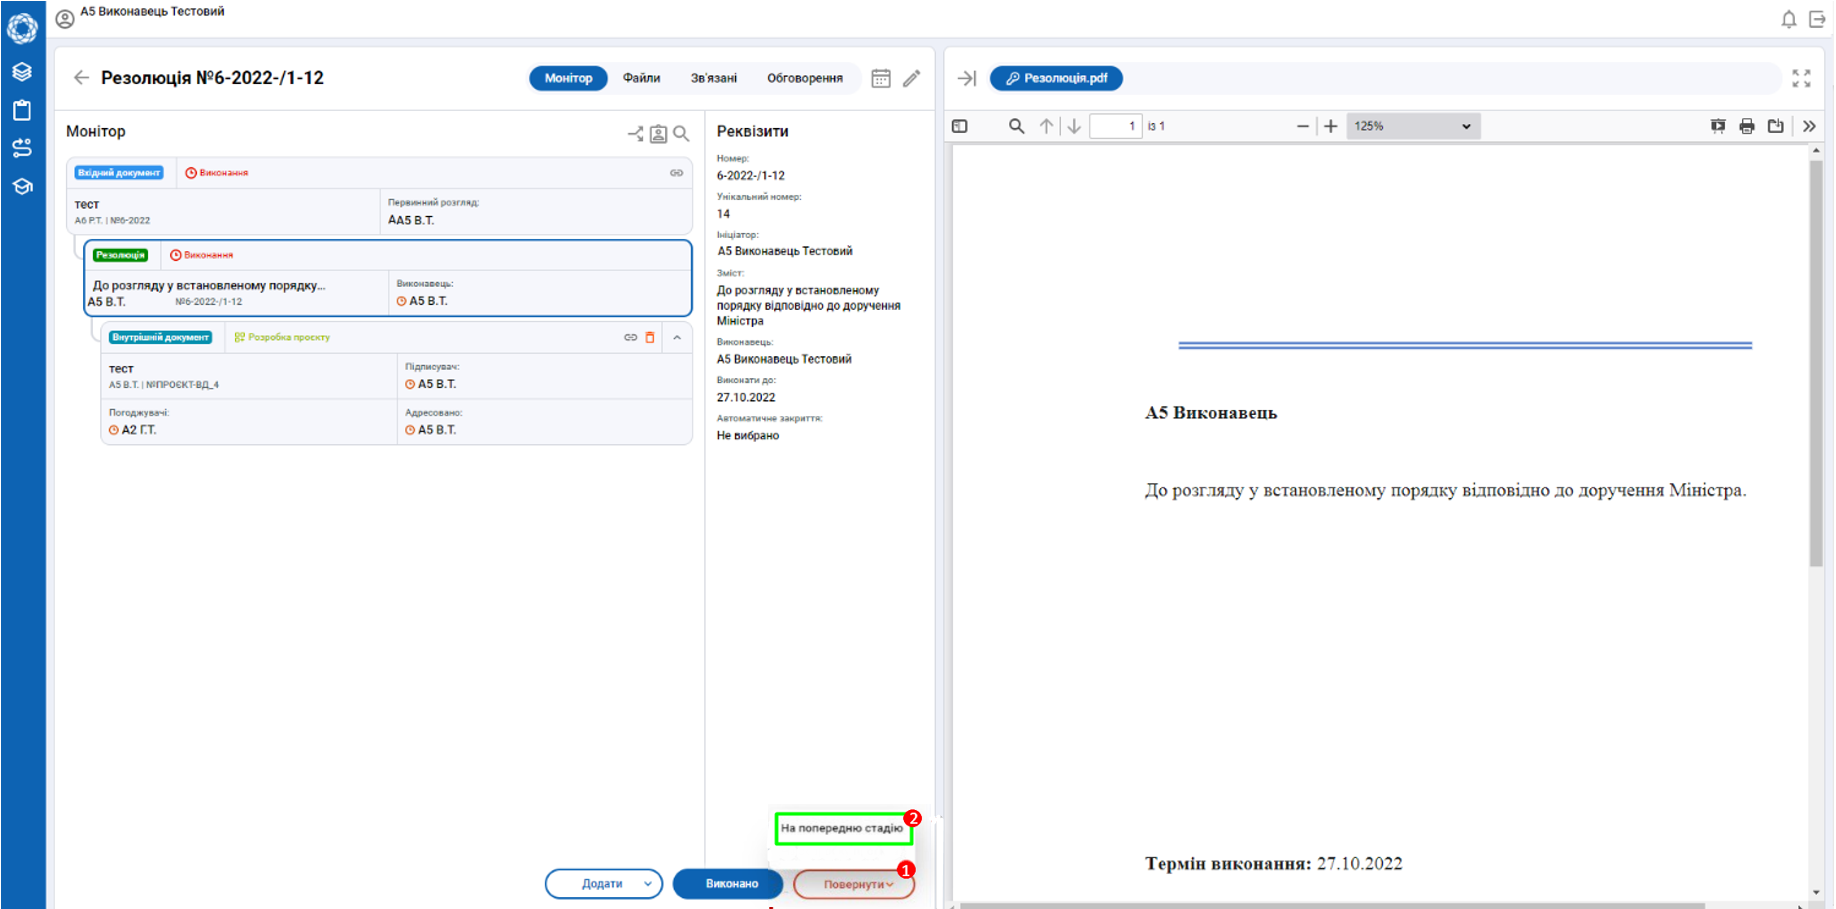
\includegraphics[width=\textwidth]{img/5.2.5.3.png}}
\caption{Рис. 5.2.5.3. Повернення документа на попередню стадію}
\end{figure}

Обов'язково вкажіть причину повернення документа:
--- «Змінити виконавця документа» → позначено цифрою \circled{1} на Рисунку 5.2.5.4
→ натисніть елемент \circled{→} → позначено цифрою \circled{2} на Рисунку 5.2.5.4.

\begin{figure}[!htbp]
\centerline{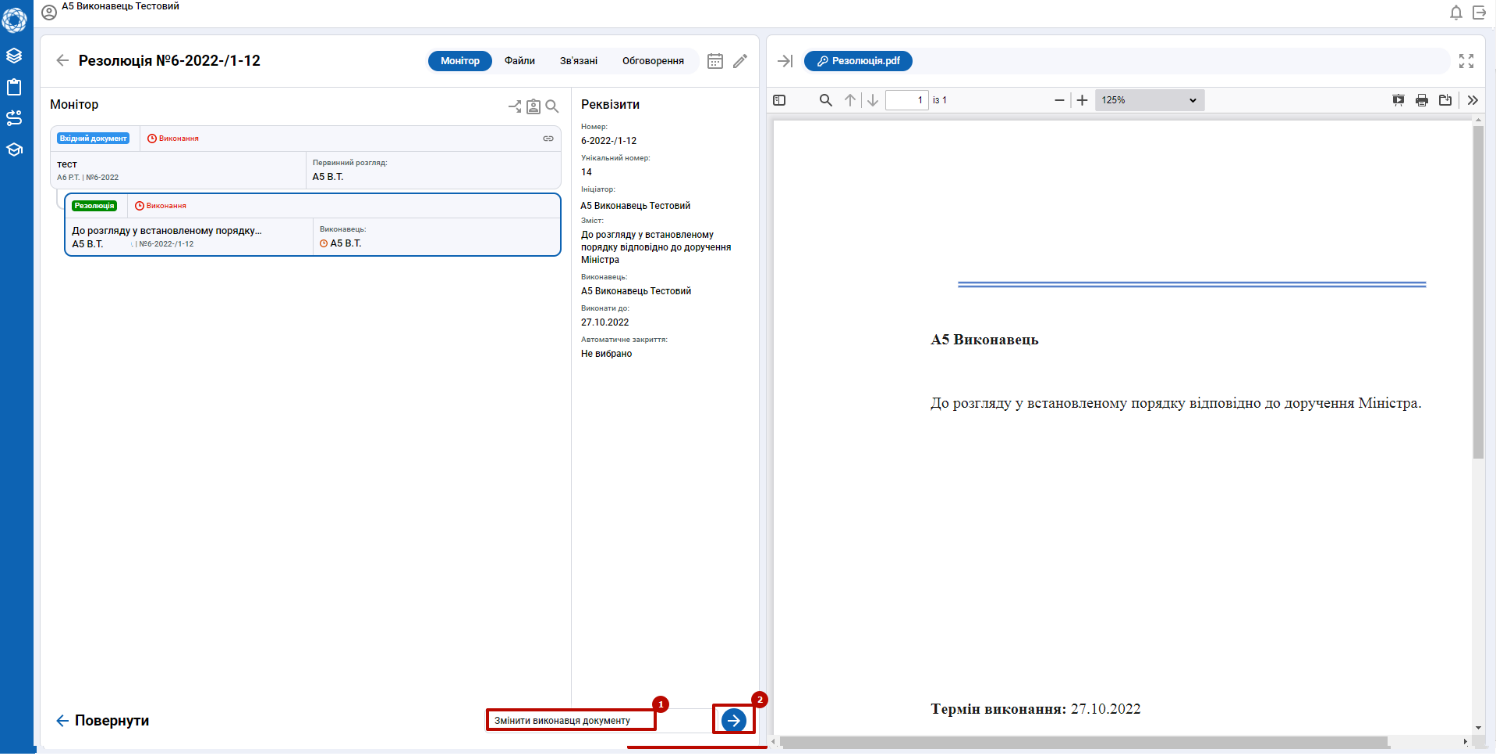
\includegraphics[width=\textwidth]{img/5.2.5.4.png}}
\caption{Рис. 5.2.5.4. Причина повернення документа}
\end{figure}

\subsection{Створення проєкту вихідного документу \\ на основі резолюції}

Для Створення проєкту вихідного документа:
--- натисніть активний елемент «Додати» → позначено цифрою \circled{1} на Рисунку 5.3.1.1;
--- \circled{→} виберіть з розгорнутого переліку «Вихідний документ» → позначено цифрою \circled{2} на Рисунку 5.3.1.1.

\begin{figure}[!htbp]
\centerline{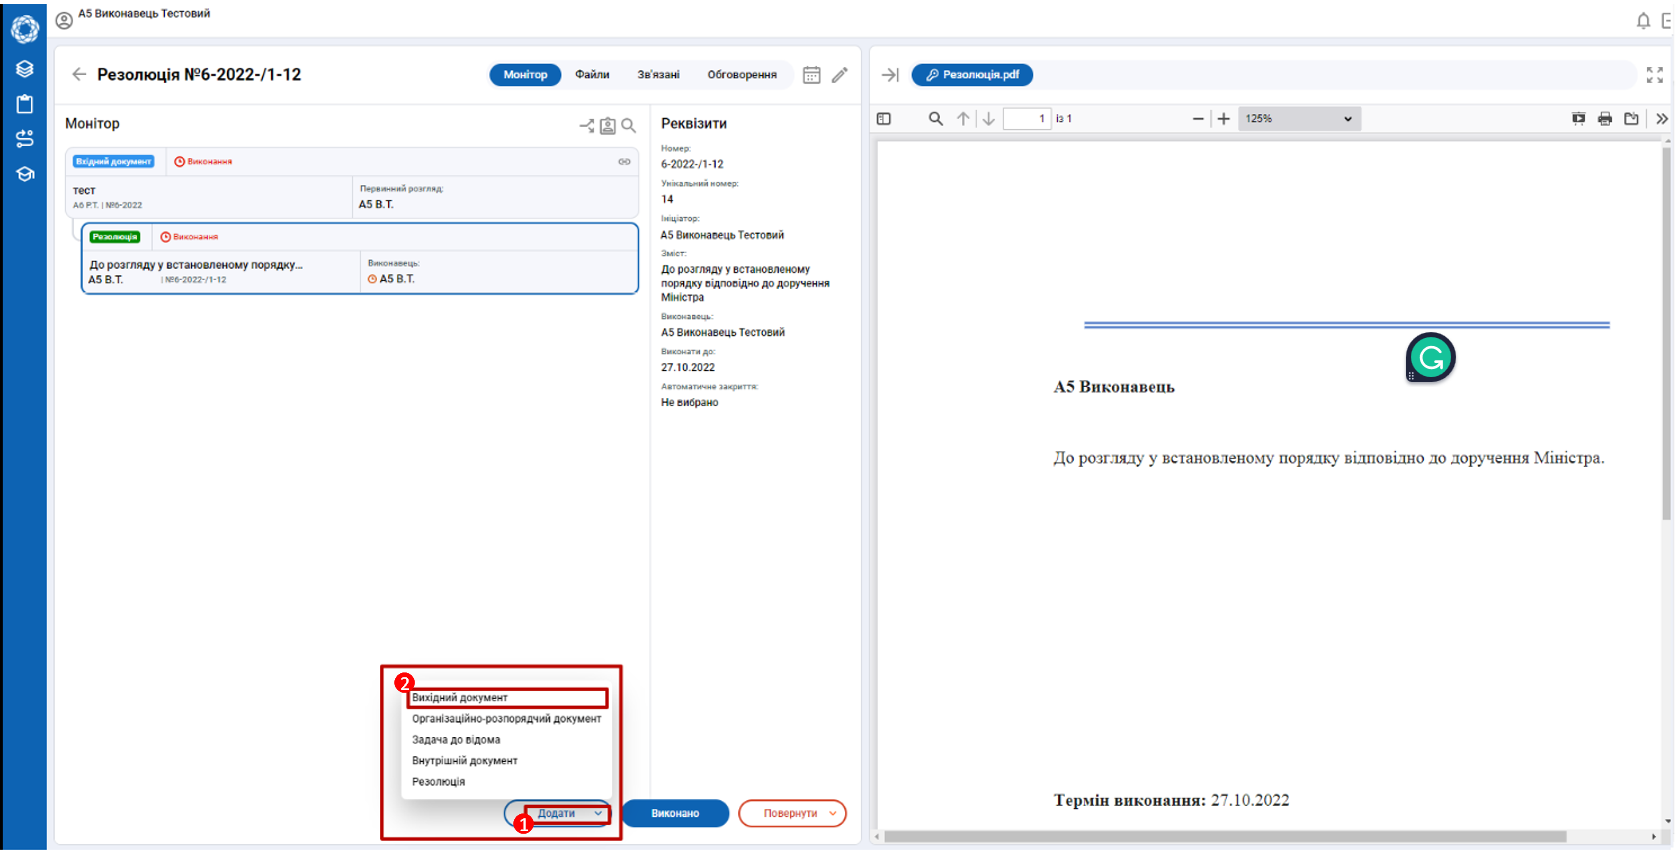
\includegraphics[width=\textwidth]{img/5.3.1.1.png}}
\caption{Рис. 5.3.1.1. Етапи створення проєкту вихідного документа}
\end{figure}

на екрані за замовчуванням відкриється підменю «Вихідний документ» →
позначено цифрою 1 на Рисунку 5.3.1.2, що являє собою область для введення даних РМК;
--- виберіть вид документа «Вихідний лист» → позначено цифрою \circled{2} на Рисунку 5.3.1.2;
--- заповніть РМК в області введення даних → позначена цифрою \circled{3} (виділена рамкою) на Рисунку 5.3.1.2;
--- важливо: поля відмічені \circled{$\ast$} обов’язкові для заповнення.

\begin{figure}[!htbp]
\centerline{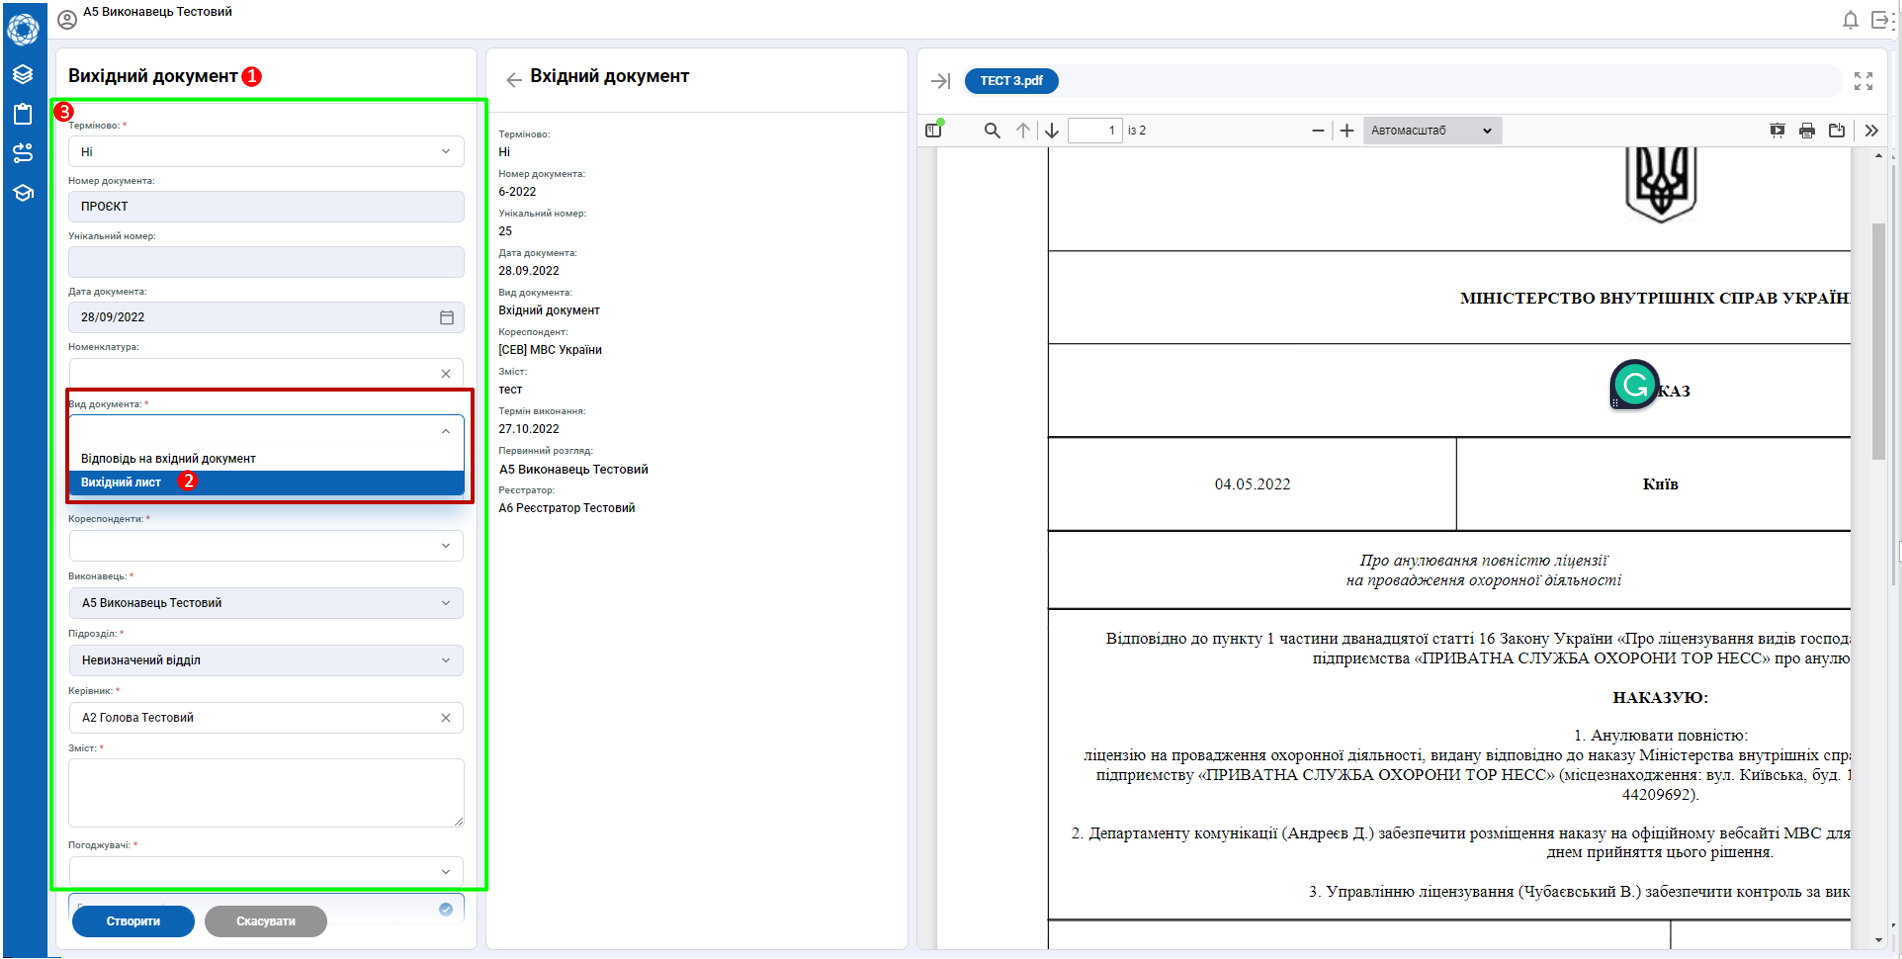
\includegraphics[width=\textwidth]{img/5.3.1.2.png}}
\caption{Рис. 5.3.1.2. Етапи створення проєкту вихідного документа}
\end{figure}

оберіть тип шаблону «Порожній вихідний документ» → позначено цифрою \circled{1} (виділено рамкою) на Рисунку 5.3.1.3;
--- натисніть активний елемент «Створити» → позначено цифрою \circled{2} на Рисунку 5.3.1.3;
--- вихідний документ успішно створено.

\begin{figure}[!htbp]
\centerline{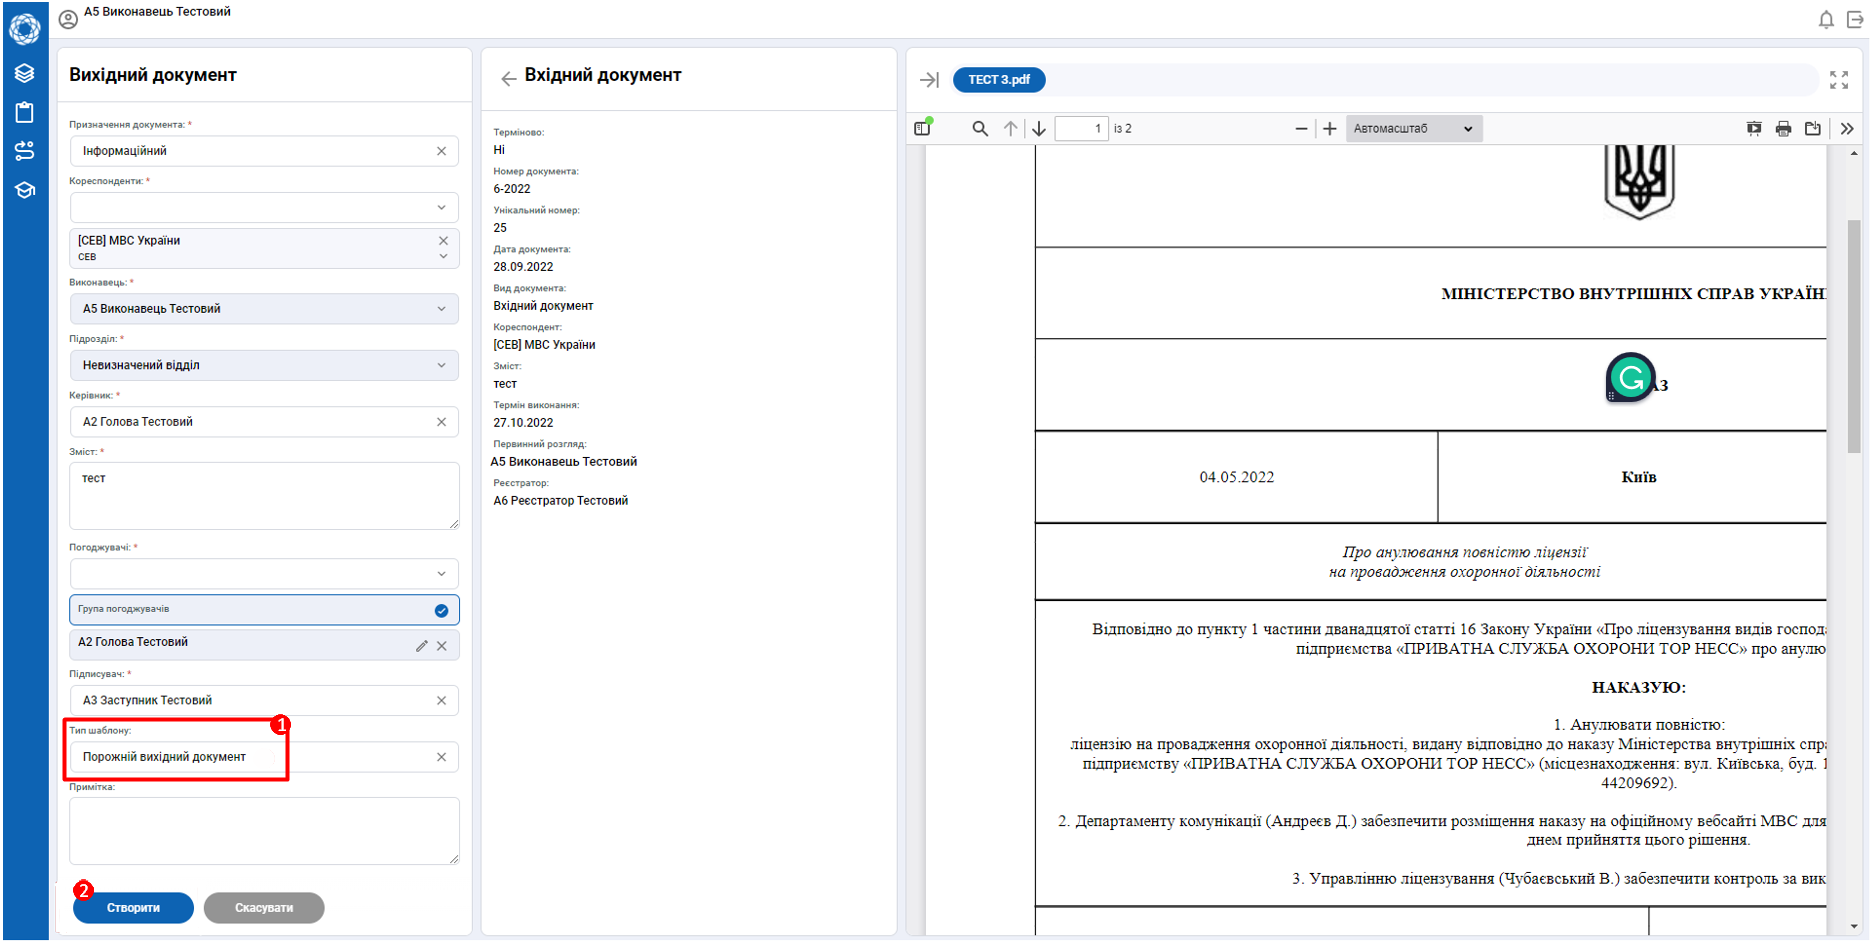
\includegraphics[width=\textwidth]{img/5.3.1.3.png}}
\caption{Рис. 5.3.1.3. Створення проєкту вихідного документа}
\end{figure}

\subsection{Редагування вихідного документу}

Після створення на попередньому етапі вихідного документа, існує
можливість змінити попередньо внесені дані (у разі необхідності) за допомогою
редагування.

Для Редагування вихідного документа:
--- відкрити меню редагування (піктограма із зображенням олівця у верхній лівій частині екранної форми);
--- користувач має змогу внести зміни наступного характеру:
1) виправити/ змінити дані в РМК → область позначена цифрою \circled{1} на Рисунку 5.3.2.1;
2) додати матеріали → (перетягнути файл/ натиснути щоб додати файл) в поле, позначене цифрою \circled{2} на Рисунку 5.3.2.1;
3) додати відскановані документи → позначено цифрою \circled{3} на Рисунку 5.3.2.1 (функціональність піктограми сканування описано в пункті 5.1.2 розділу 5);
4) заповнити шаблон/ відредагувати доданий файл (якщо він у форматі $\ast$.docx) → область позначена цифрою \circled{4} на Рисунку 5.3.2.1;
5) після внесення відповідних змін → натисніть піктограму «Зберегти» → позначено цифрою \circled{5} на Рисунку 5.3.2.1.

\begin{figure}[!htbp]
\centerline{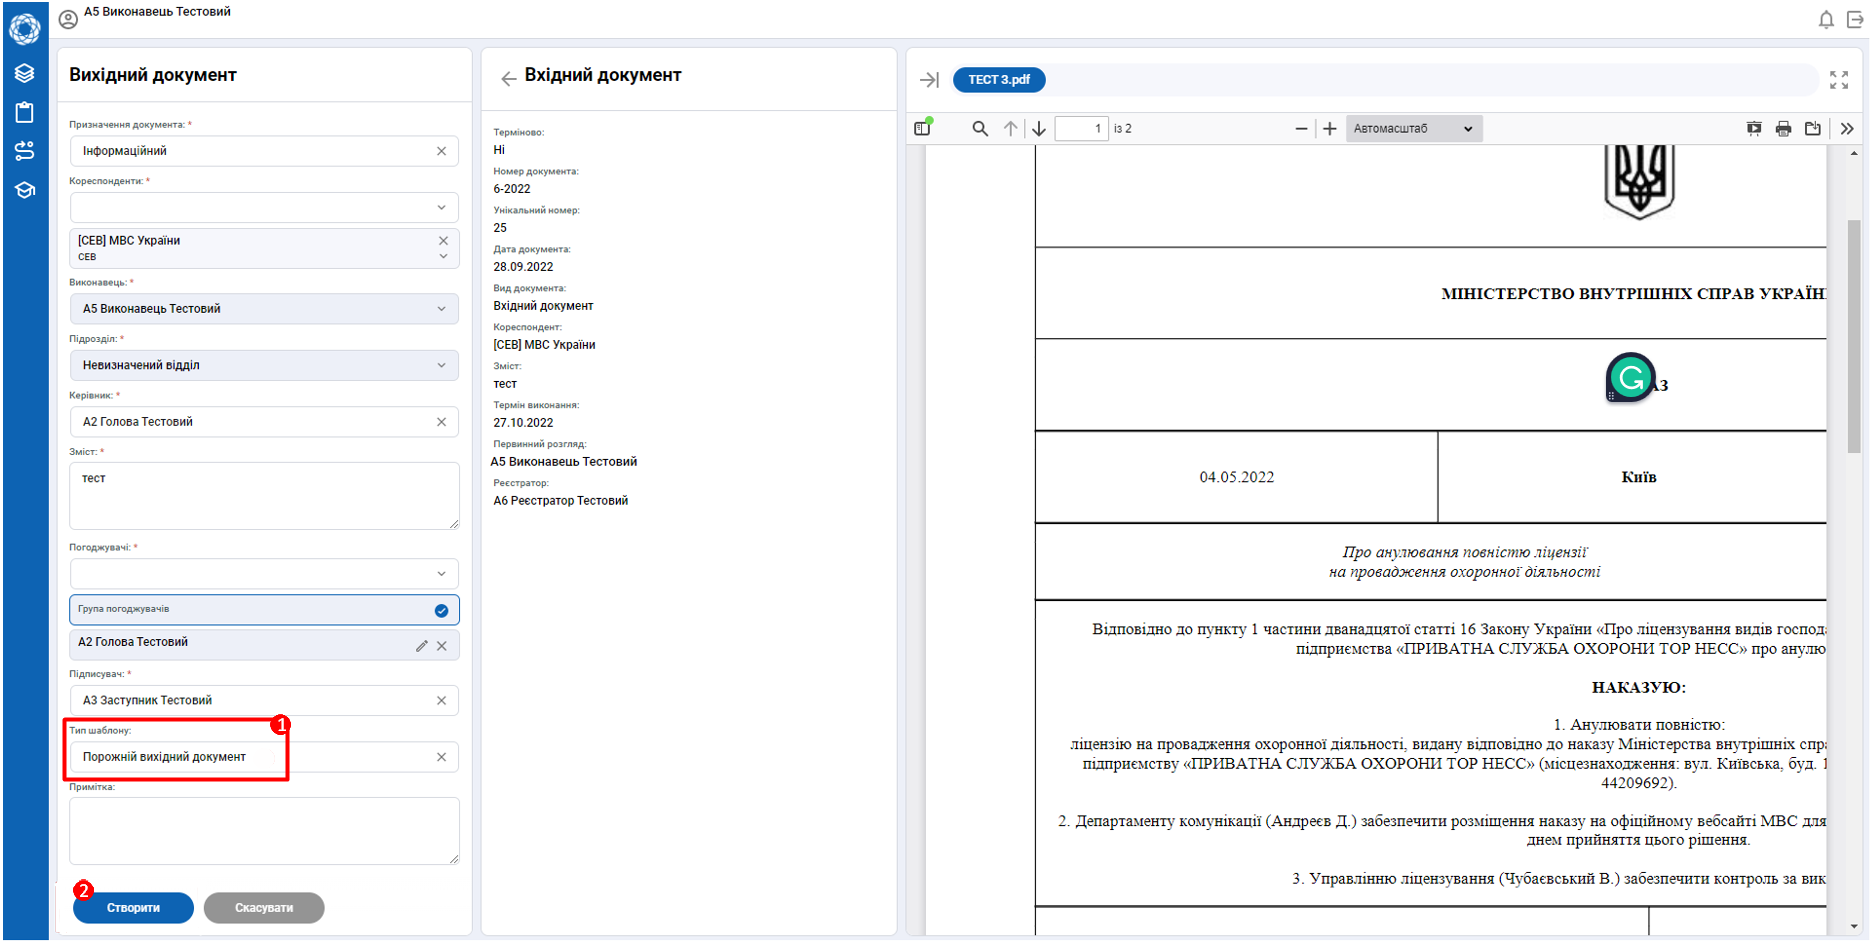
\includegraphics[width=\textwidth]{img/5.3.1.3.png}}
\caption{Рис. 5.3.2.1. Процес внесення змін у документ}
\end{figure}

щоб підтвердити введення змін → натисніть активний елемент «Змінити» → позначено червоною рамкою на Рисунку 5.3.2.2

\begin{figure}[!htbp]
\centerline{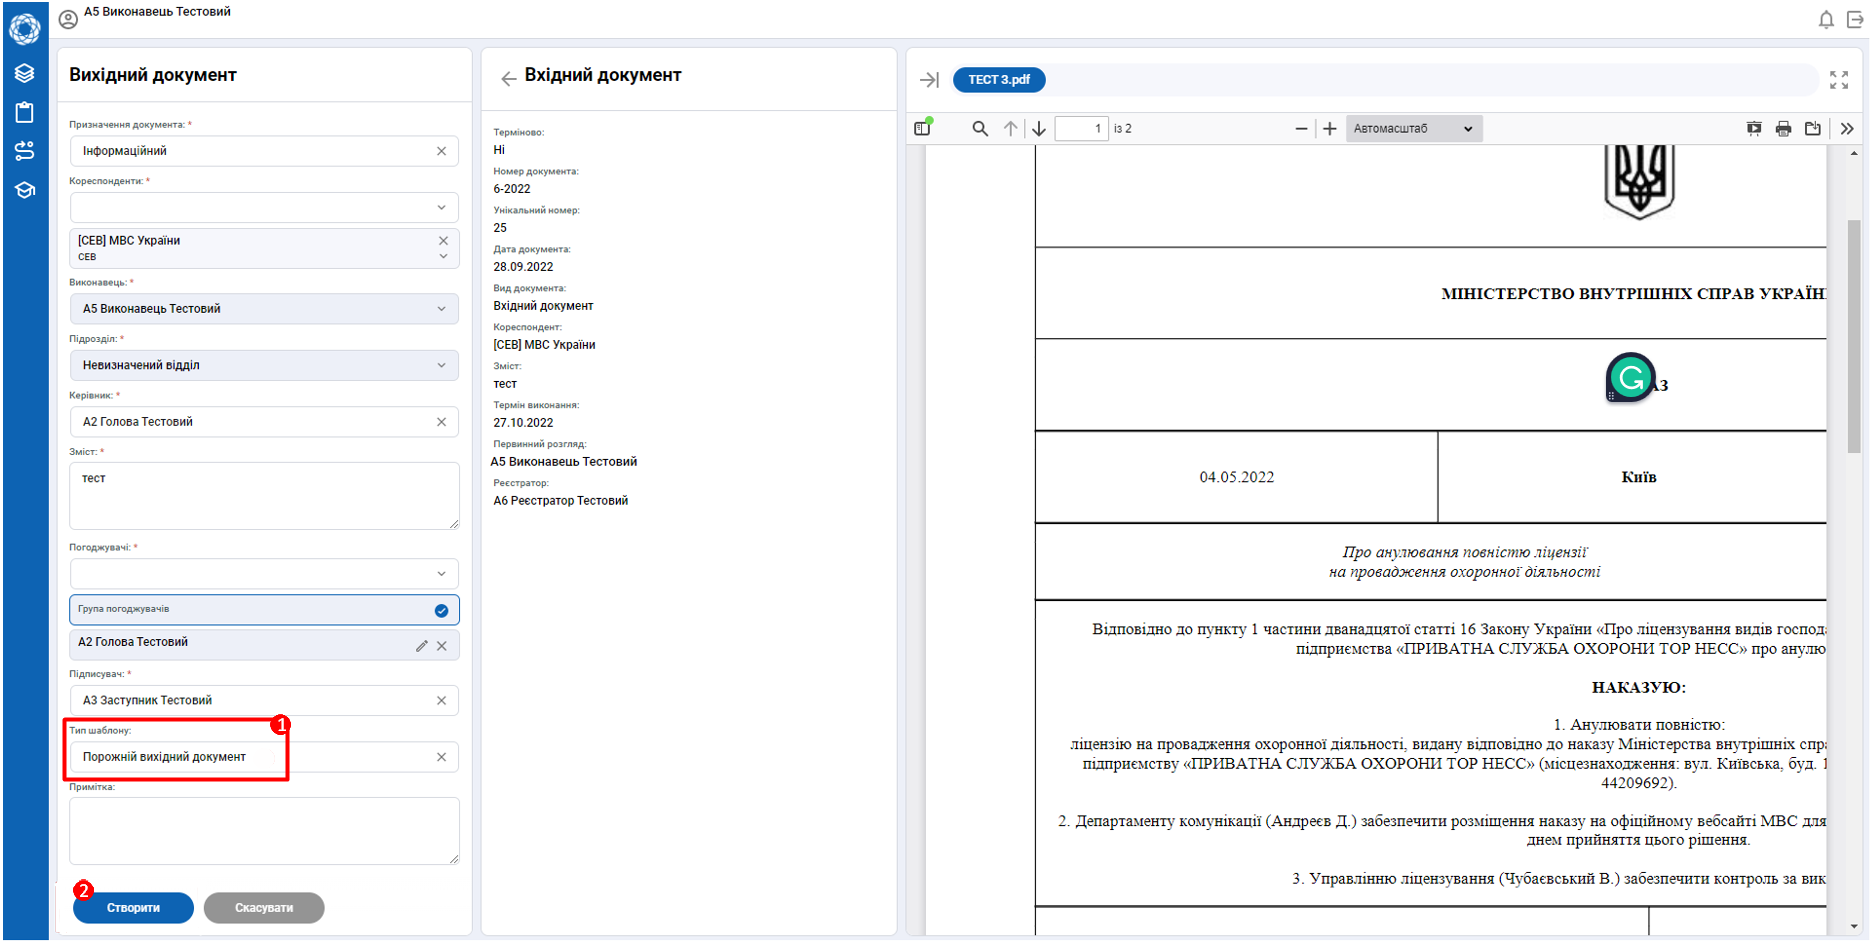
\includegraphics[width=\textwidth]{img/5.3.1.3.png}}
\caption{Рис. 5.3.2.2. Завершальний етап внесення змін у документ}
\end{figure}

\subsection{Видалення проєкту вихідного документа}

Для Видалення проєкту вихідного документа:
--- Натисніть піктограму «Видалити» → позначено цифрою \circled{1} на Рисунку 5.3.3.1.

\begin{figure}[!htbp]
\centerline{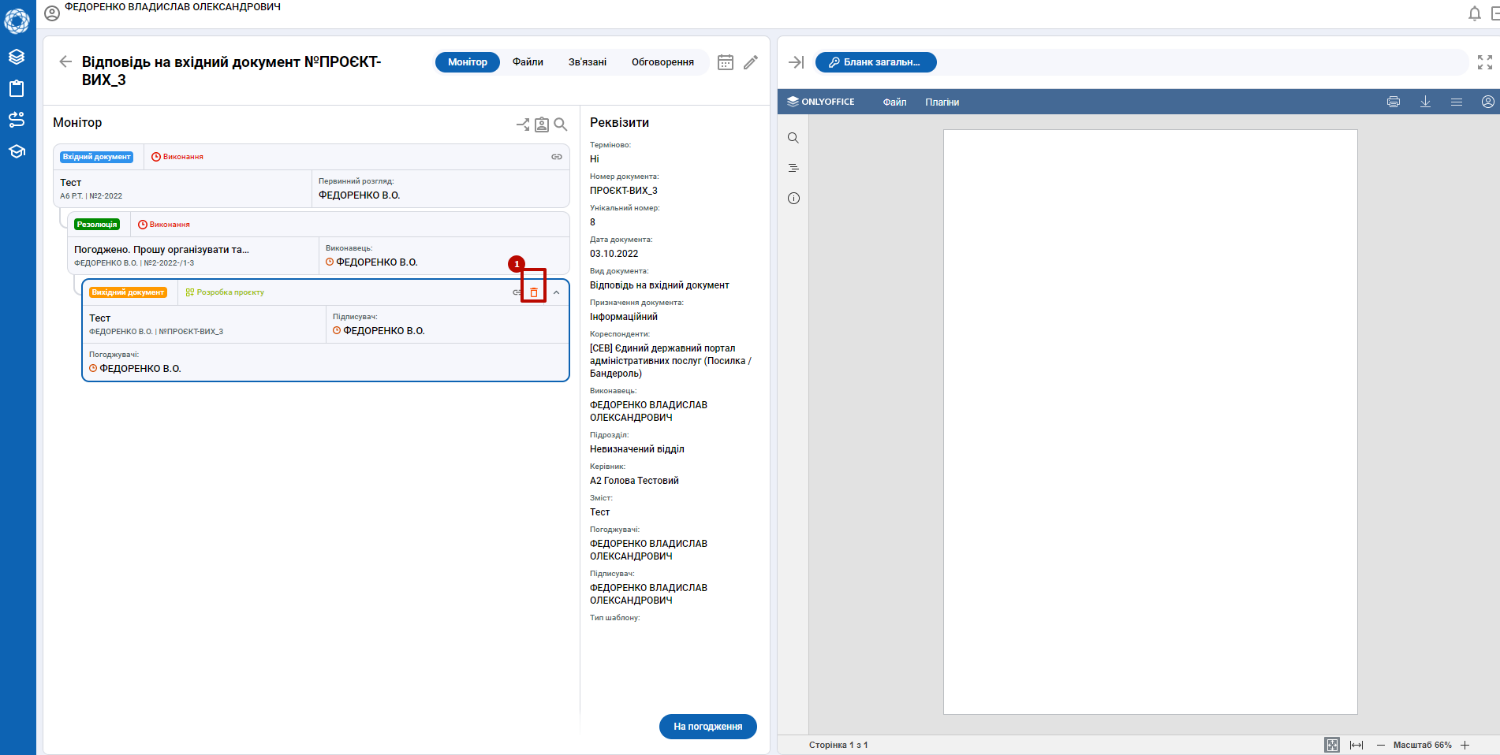
\includegraphics[width=\textwidth]{img/5.3.3.1.png}}
\caption{Рис. 5.3.3.1. Видалення проєкту вихідного документа}
\end{figure}

Після Завершення роботи (створення/ редагування) над проєктом вихідного документа:
--- натисніть активний елемент «На погодження» → позначено цифрою \circled{1} на Рисунку 5.3.3.2;
--- список/ порядок погодження визначається в процесі заповнення РМК.

\begin{figure}[!htbp]
\centerline{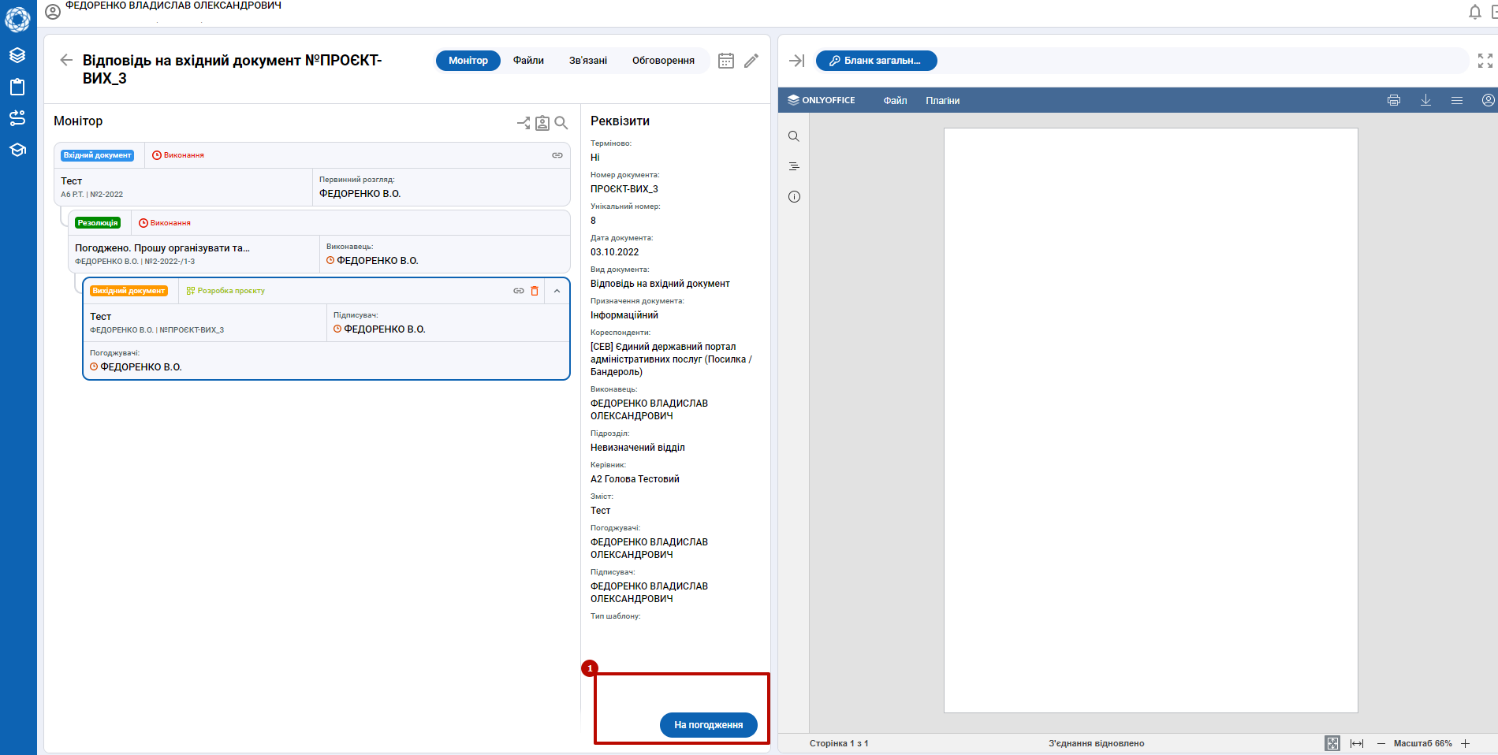
\includegraphics[width=\textwidth]{img/5.3.3.2.png}}
\caption{Рис. 5.3.3.2. Погодження}
\end{figure}

\section{Внутрішній документ}

\subsection{Створення проєкту \\ на основі резолюції}

Для Створення проєкту внутрішнього документа:
--- натисніть елемент «Додати» → позначено цифрою \circled{1} на Рисунку 5.4.1.1;
--- з розгорнутого переліку \circled{2} виберіть «Внутрішній документ» → позначено цифрою \circled{3} на Рисунку 5.4.1.1.

\begin{figure}[!htbp]
\centerline{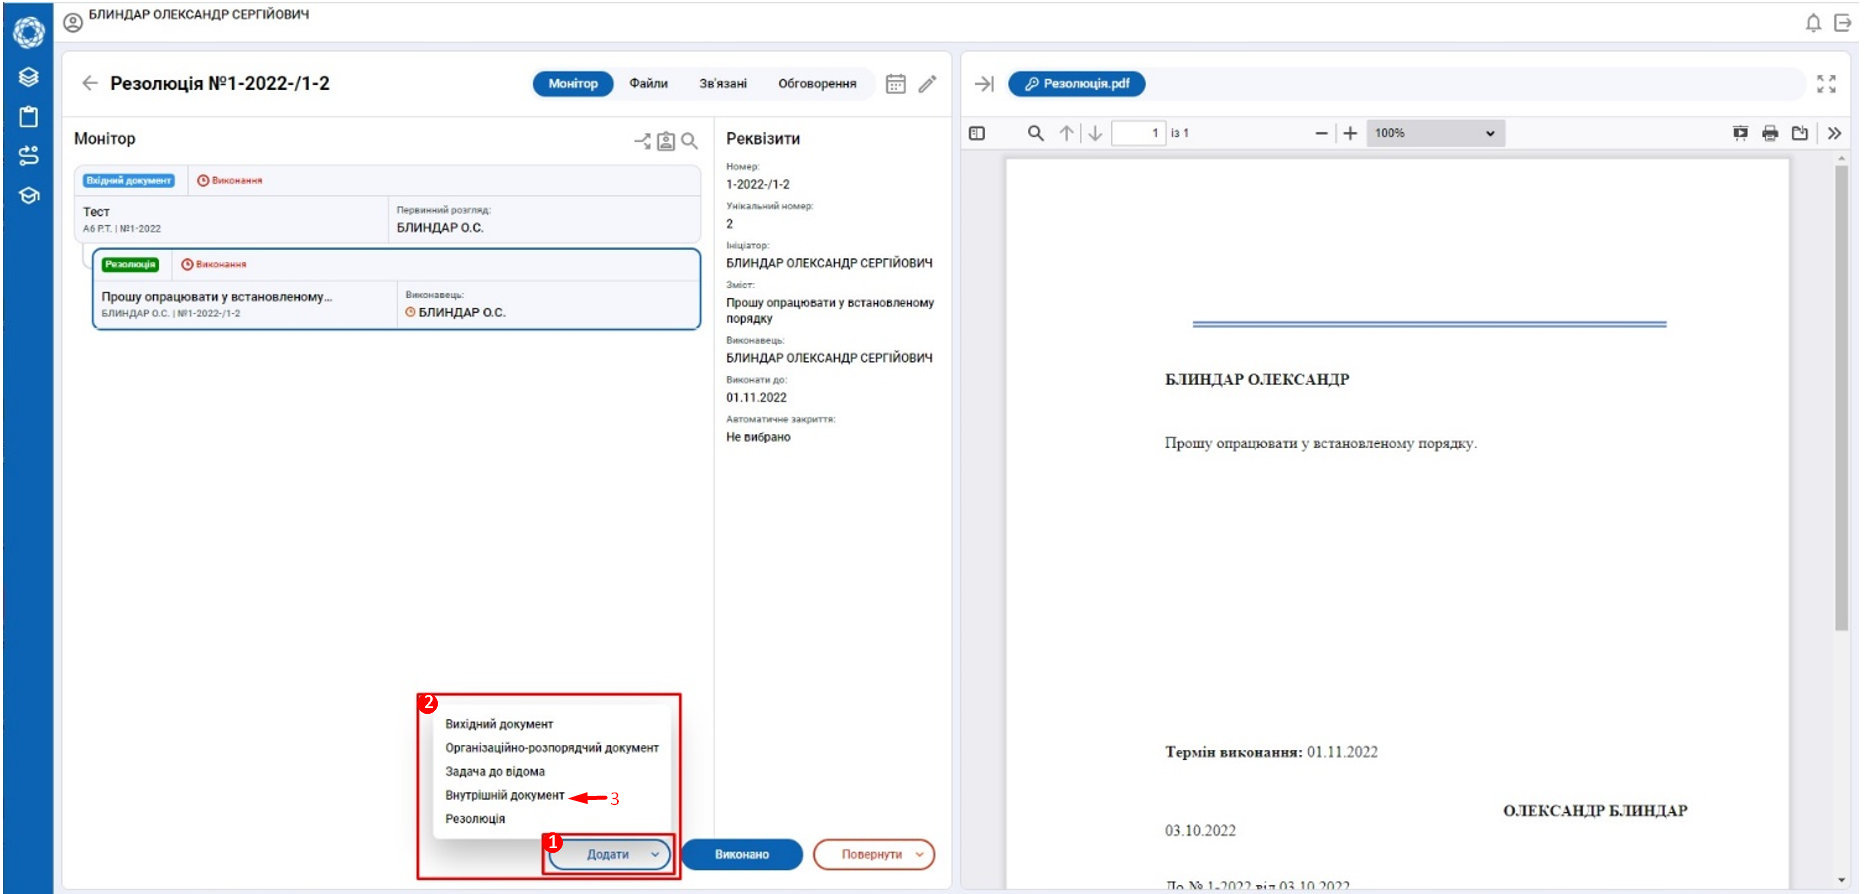
\includegraphics[width=\textwidth]{img/5.4.1.1.png}}
\caption{Рис. 5.4.1.1. Створення проєкту внутрішнього документа}
\end{figure}


--- заповніть РМК – область позначена цифрою 1 на Рисунку 5.4.1.2 (поля
відмічені \circled{$\ast$} – обов’язкові для заповнення).

\begin{figure}[!htbp]
\centerline{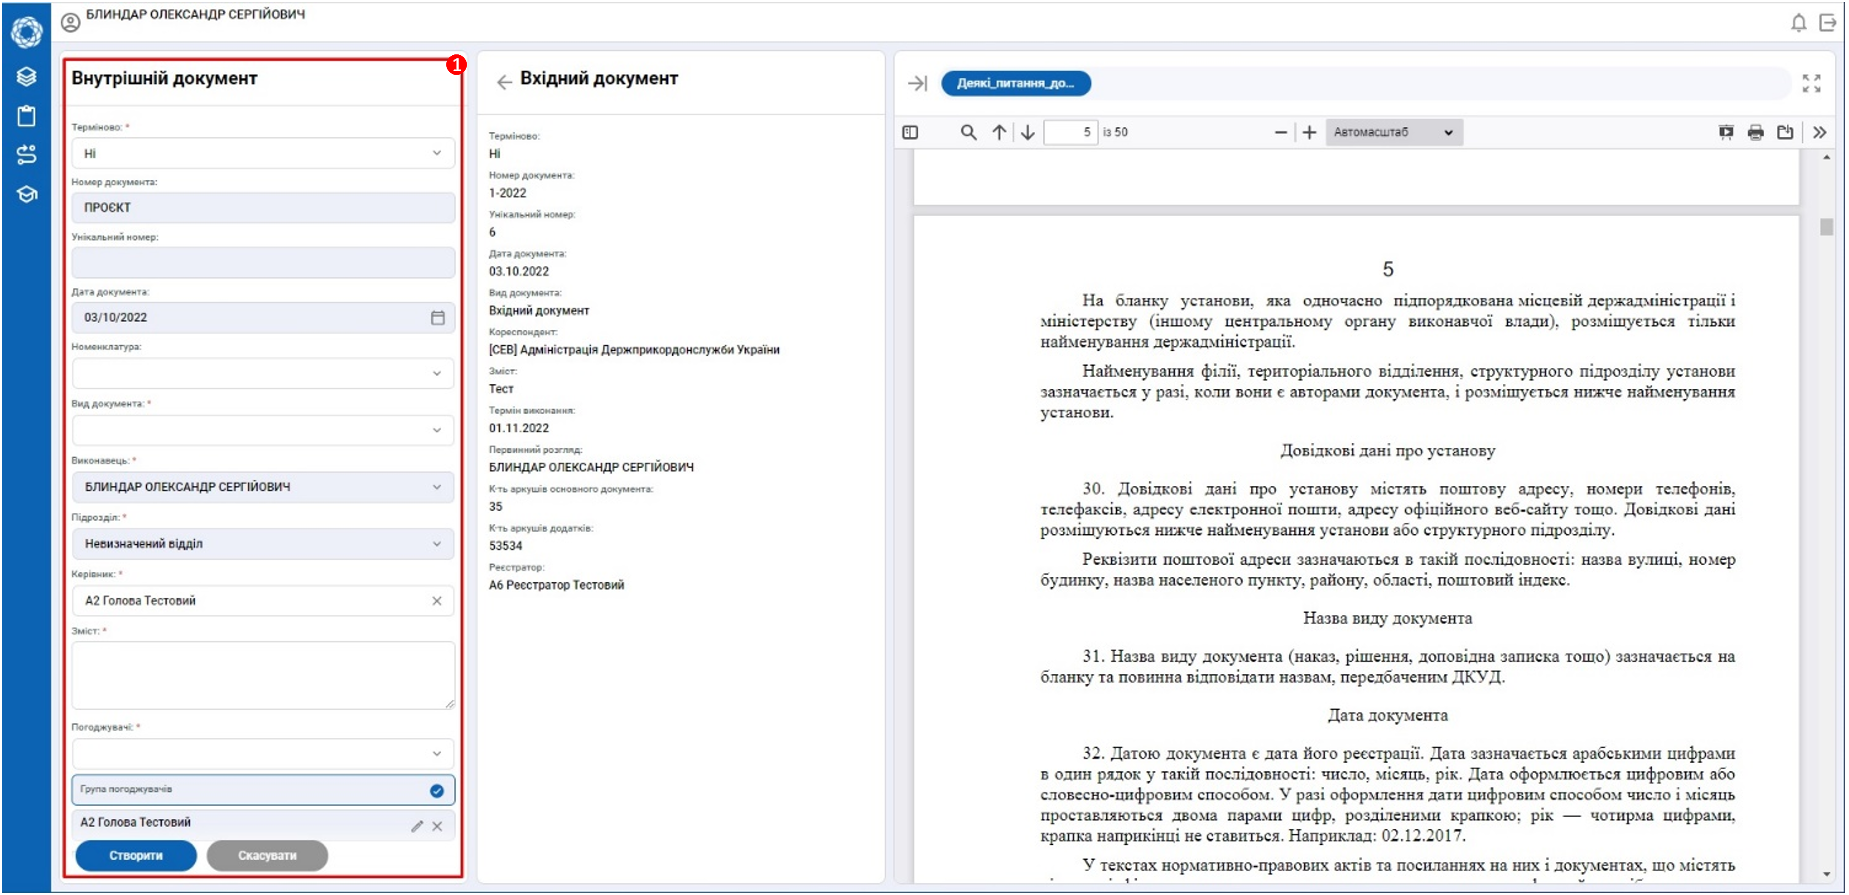
\includegraphics[width=\textwidth]{img/5.4.1.2.png}}
\caption{Рис. 5.4.1.2. }
\end{figure}

--- оберіть з розгорнутого переліку тип шаблону документа → (область вибору позначена рамкою на Рисунку 5.4.1.3);
--- або завантажте підготовлений документ із власного ПК.

\begin{figure}[!htbp]
\centerline{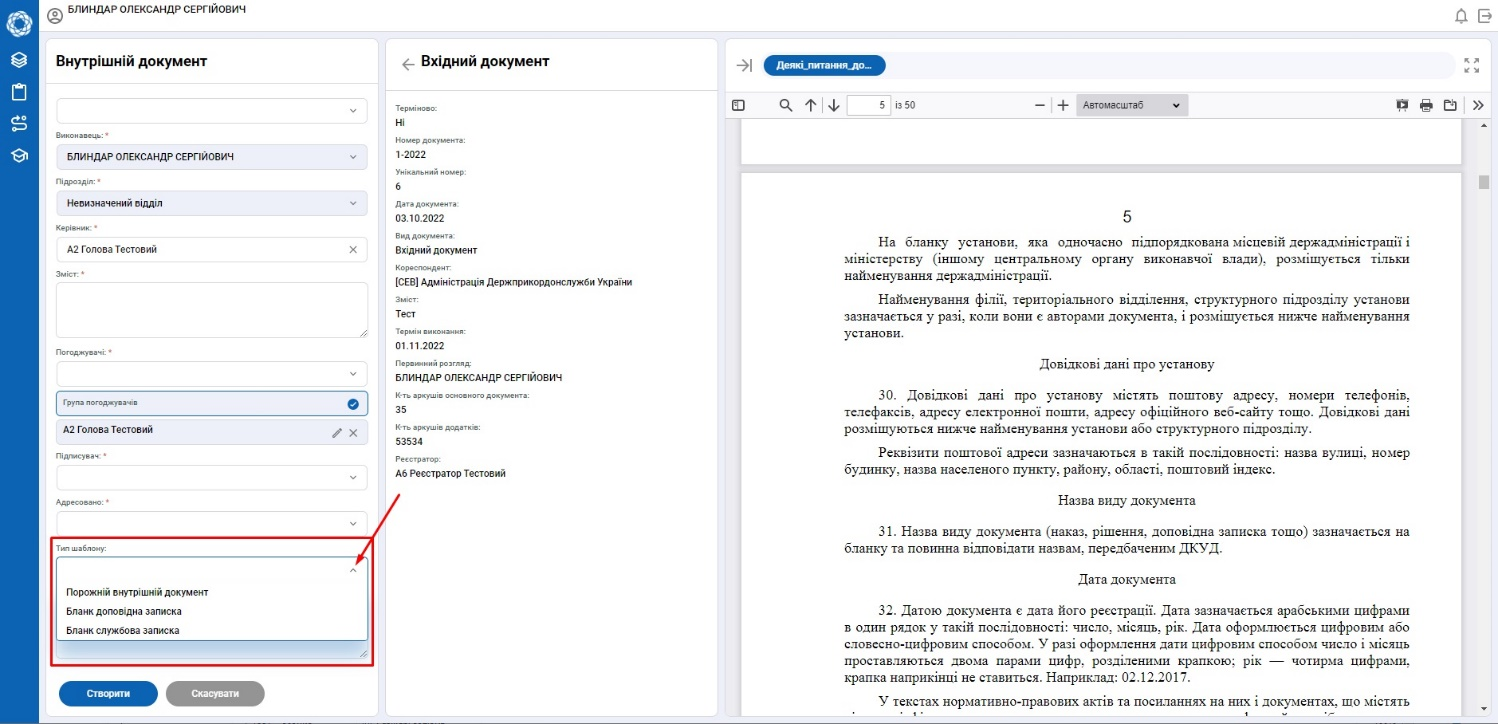
\includegraphics[width=\textwidth]{img/5.4.1.3.jpg}}
\caption{Рис. 5.4.1.3. }
\end{figure}

для завершення створення документа → натисніть активний елемент
«Створити» → (див. виділені червоним елементи на Рисунку 5.4.1.4).

\begin{figure}[!htbp]
\centerline{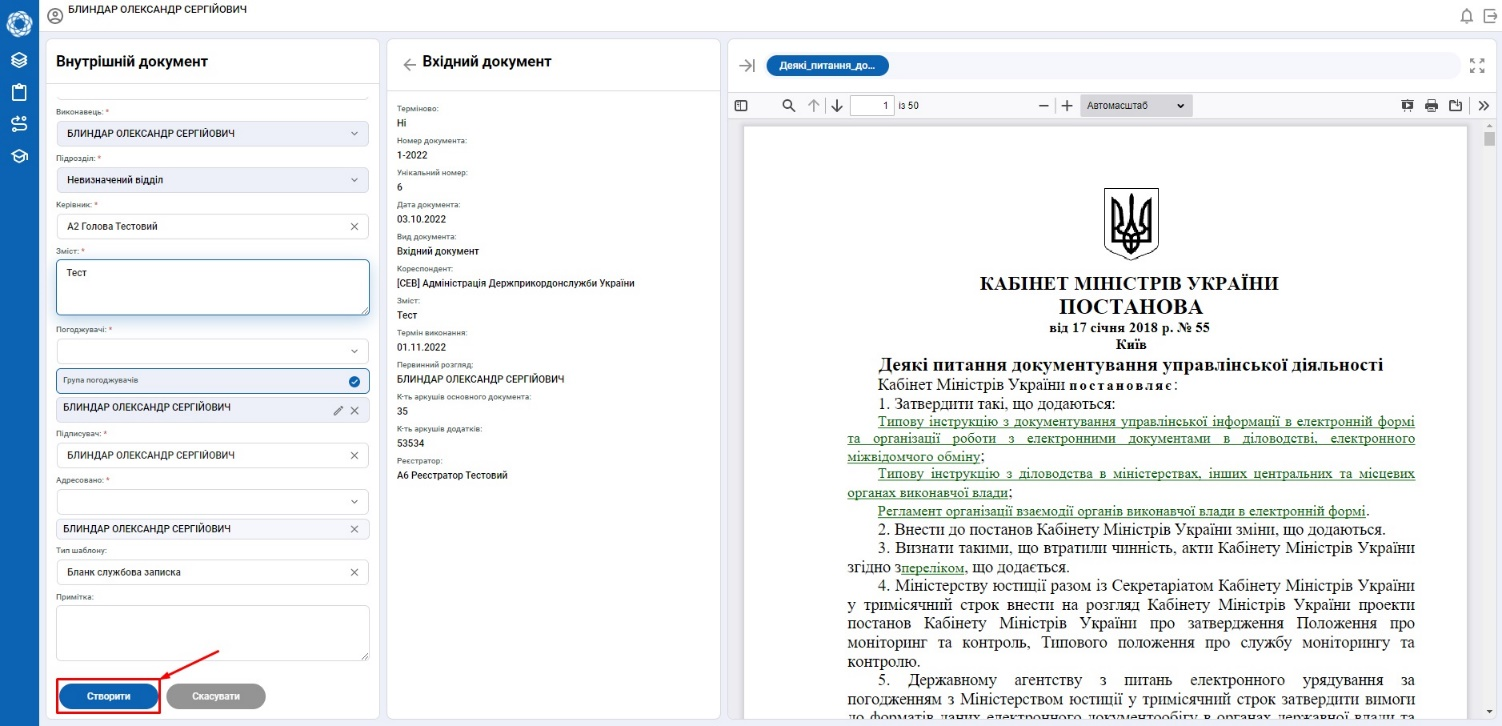
\includegraphics[width=\textwidth]{img/5.4.1.4.jpg}}
\caption{Рис. 5.4.1.4. Завершення створення проєкту внутрішнього документу з резолюції}
\end{figure}

\subsection{Редагування проєкту \\ на основі резолюції}

Для Внесення змін в проєкт внутрішнього документу:
--- відкрийте меню редагування → піктограма із зображенням олівця,
позначена червоною рамкою на Рисунку 5.4.2.1.

\begin{figure}[!htbp]
\centerline{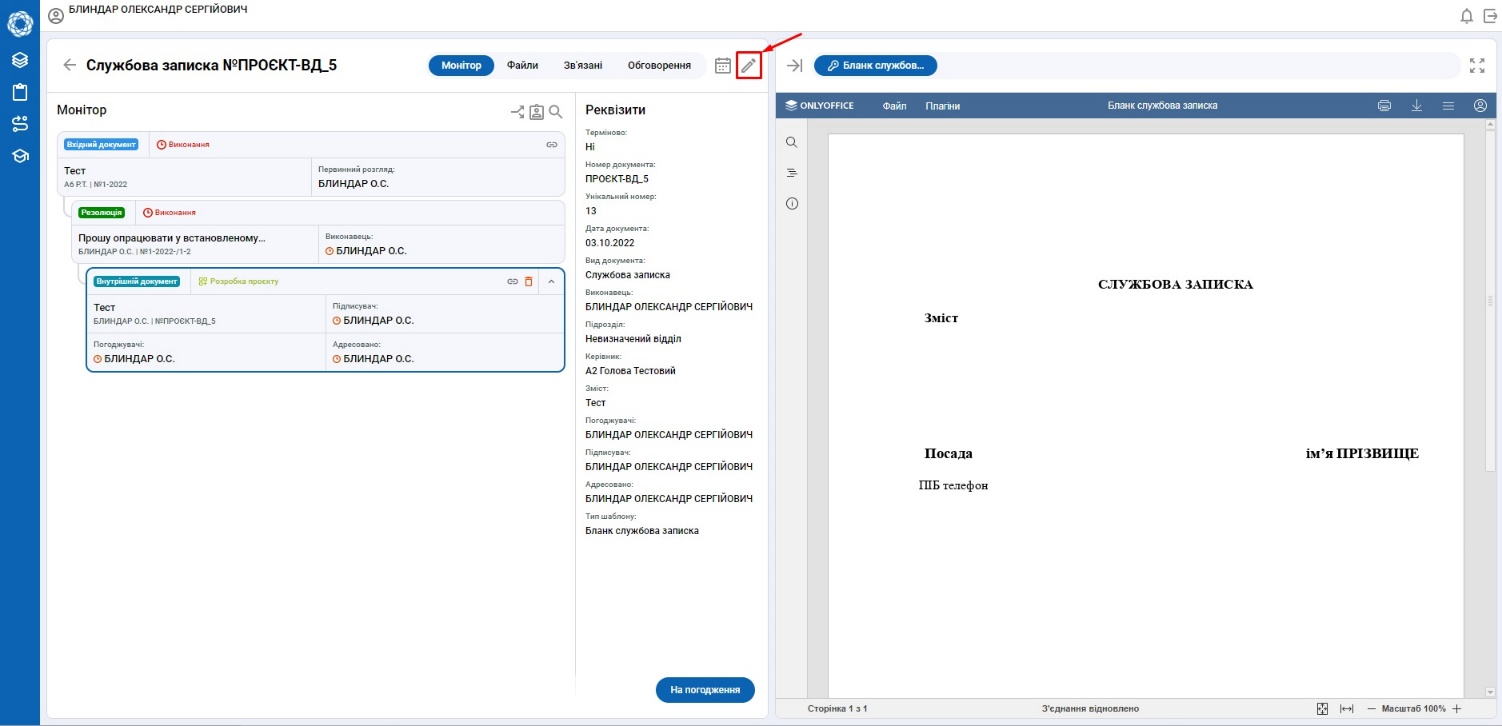
\includegraphics[width=\textwidth]{img/5.4.2.1.jpg}}
\caption{Рис. 5.4.2.1. Активація меню Редагування}
\end{figure}

Меню редагування дозволяє :
1 – внести необхідні зміни в інформаційні поля РМК;
2 – додати матеріали;
3 – відсканувати додаткові матеріали;
4 – відредагувати/ заповнити шаблон/ доданий файл, що він у форматі *.docx.;
--- умовні позначення меню редагування (відмічені цифрами) представлені на Рисунку 5.4.2.2;

\begin{figure}[!htbp]
\centerline{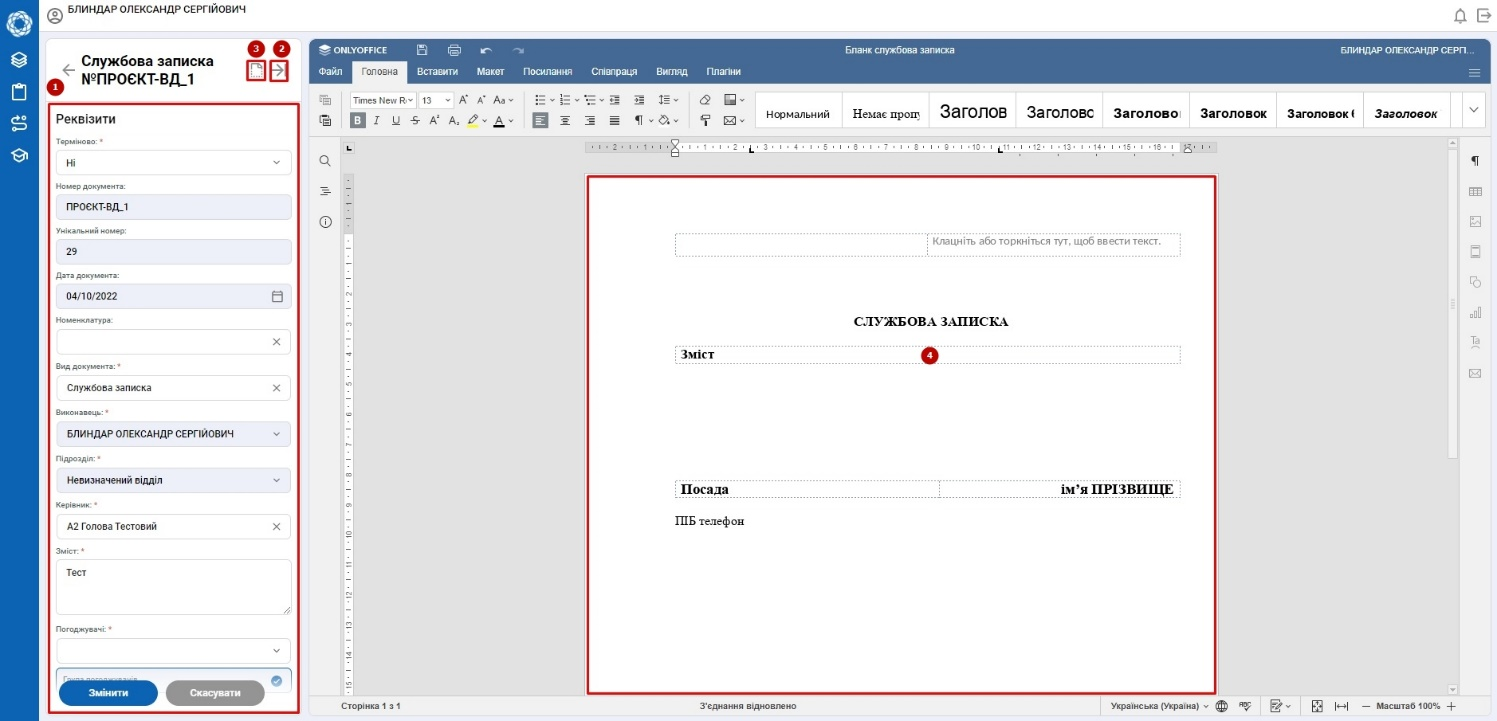
\includegraphics[width=\textwidth]{img/5.4.2.2.jpg}}
\caption{Рис. 5.4.2.2. Умовні позначення меню редагування}
\end{figure}

щоб відредагувати доданий шаблон/ доданий файл → внесіть зміни в проєкт
документа → натисніть піктограму «Зберегти» → позначено цифрою \circled{1} на Рисунку 5.4.2.3;
--- в нижній частині екранної форми вікна OnlyOffice з'явиться інформація «Усі зміни збережено»
→ позначено цифрою \circled{2} на Рисунку 5.4.2.3.

\begin{figure}[!htbp]
\centerline{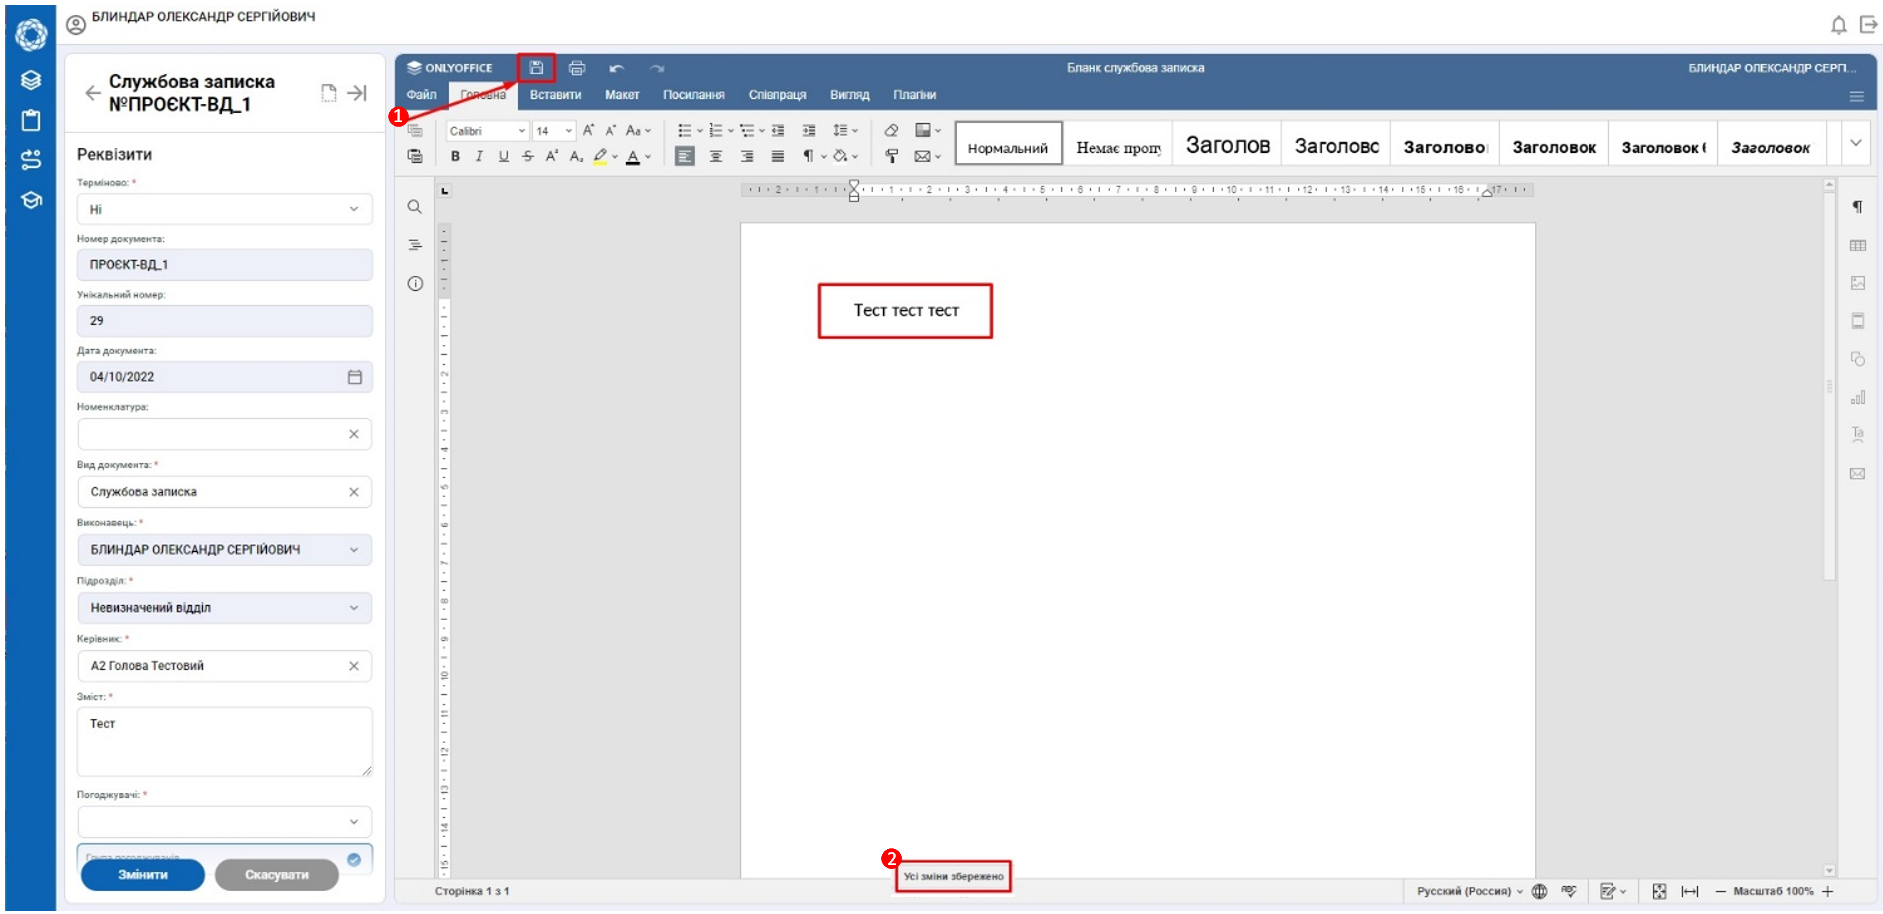
\includegraphics[width=\textwidth]{img/5.4.2.3.png}}
\caption{Рис. 5.4.2.3. Збереження змін у проєкт документа}
\end{figure}

щоб вибрати основний документ а також документи, що потребують підпису
→ відмітьте позначкою чек-бокс «Зробити основним» та/або «Потребує
підпису» → область вибору виділена червоною рамкою на Рисунку 5.4.2.4;
--- примітка: для шаблонів Системи цей пункт обрано за замовчуванням.

\begin{figure}[!htbp]
\centerline{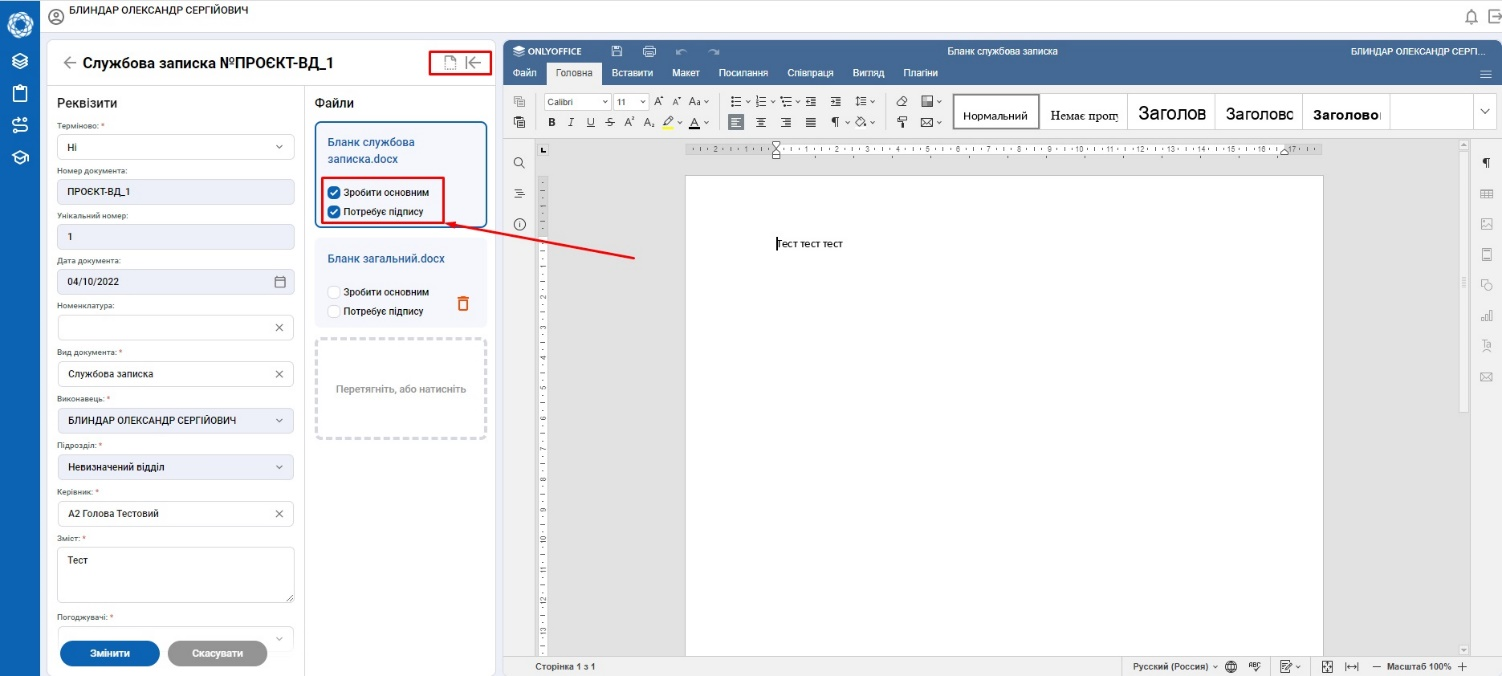
\includegraphics[width=\textwidth]{img/5.4.2.4.jpg}}
\caption{Рис. 5.4.2.4. }
\end{figure}

щоб підтвердити зміни → натисніть активний елемент «Змінити» →
позначений червоною рамкою на Рисунку 5.4.2.5.

\begin{figure}[!htbp]
\centerline{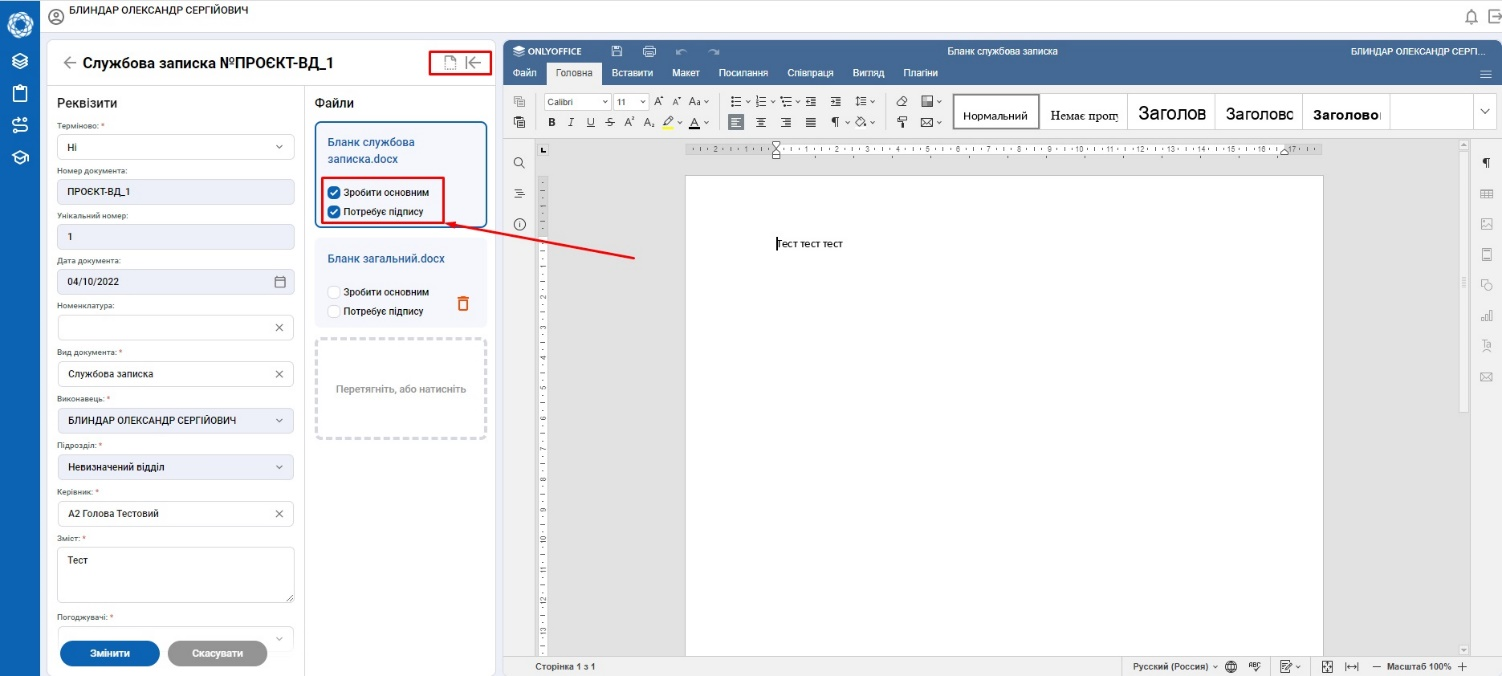
\includegraphics[width=\textwidth]{img/5.4.2.4.jpg}}
\caption{Рис. 5.4.2.5. Закінчення роботи з проєктом внутрішнього документа}
\end{figure}

\subsection{Видалення проєкту \\ на основі резолюції}

Для Видалення проєкту внутрішнього документа:
--- натисніть піктограму «Видалити» → виділена червоним на Рисунку 5.4.3.1

\begin{figure}[!htbp]
\centerline{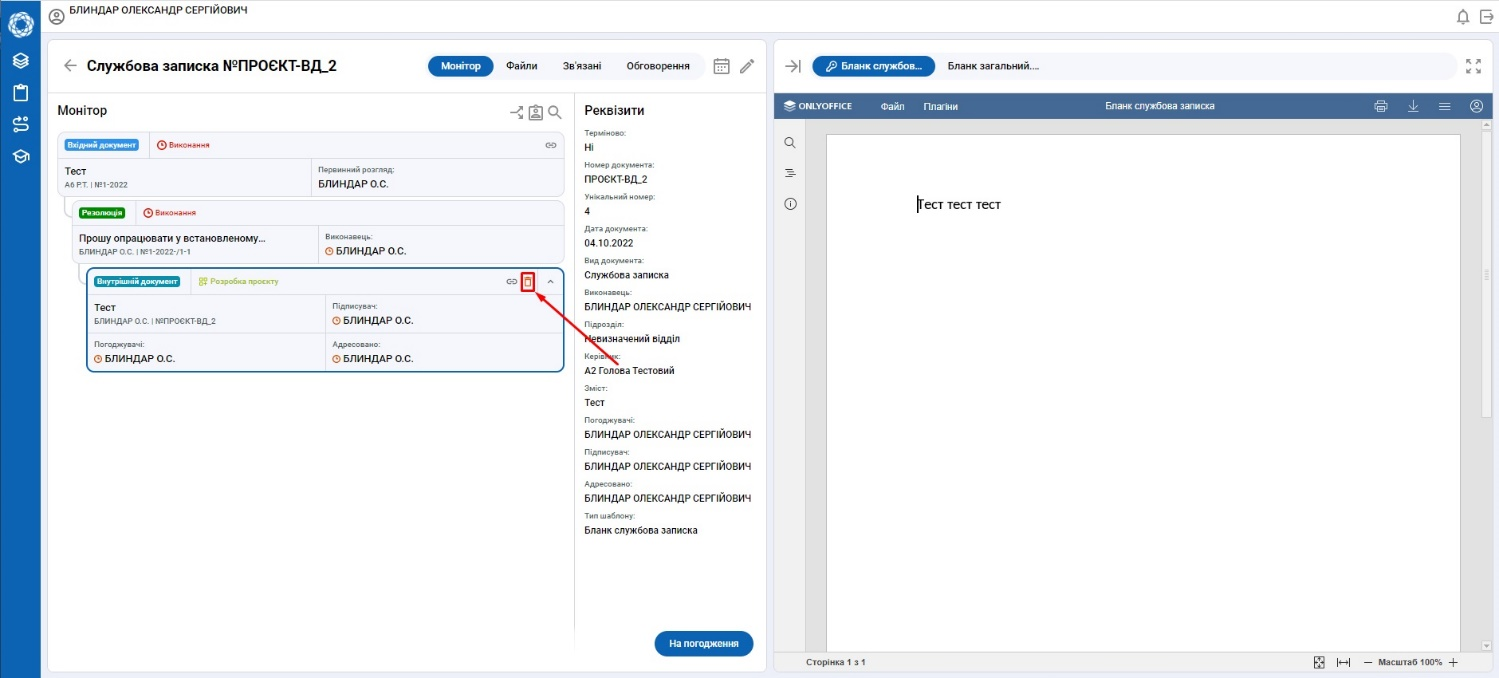
\includegraphics[width=\textwidth]{img/5.4.3.1.jpg}}
\caption{Рис. 5.4.3.1. Видалення проєкту внутрішнього документа}
\end{figure}

у підсумку процеси створення/ редагування проєкта внутрішнього
документа закінчуються переходом на стадію «Погодження» (згідно списку
погодження, що було визначено в процесі заповнення РМК).
--- Для погодження документа → натисніть активний елемент «На
погодження» → позначений червоною рамкою на Рисунку 5.4.3.2.

\begin{figure}[!htbp]
\centerline{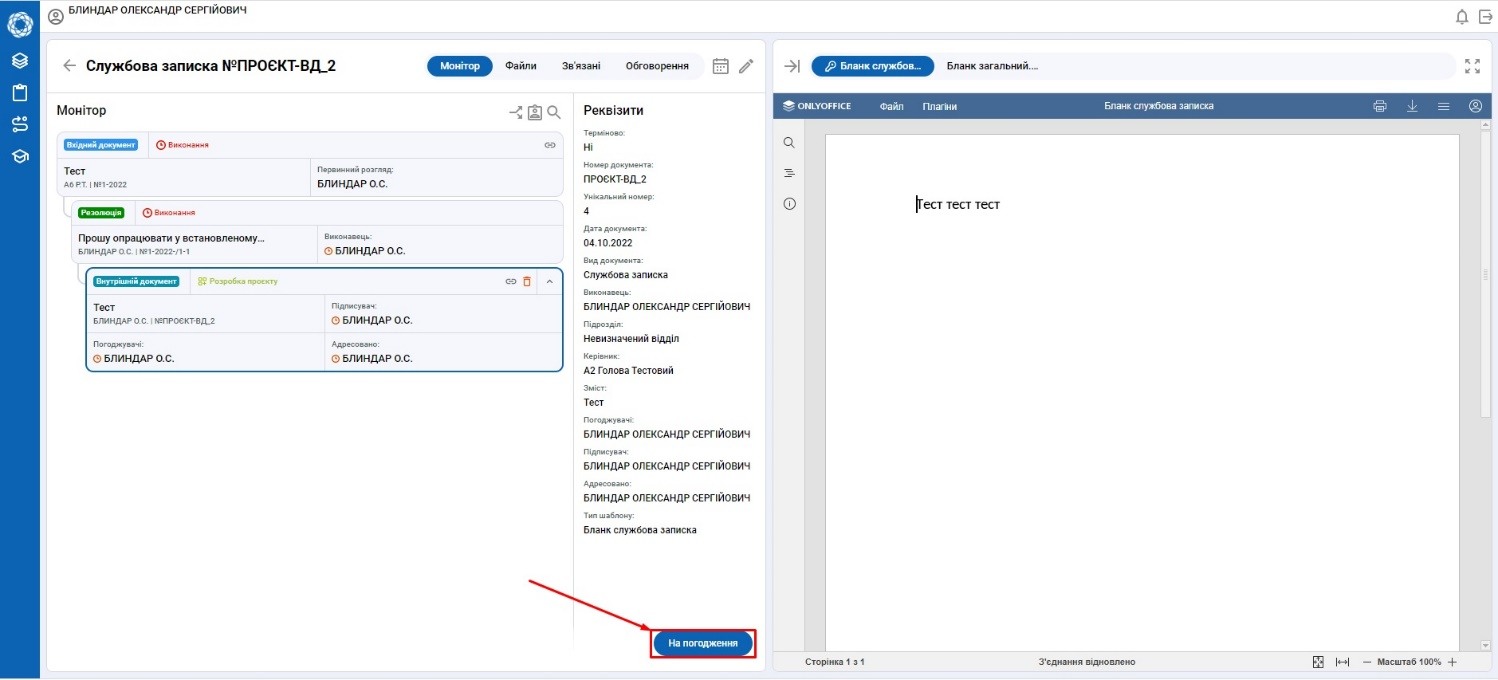
\includegraphics[width=\textwidth]{img/5.4.3.2.jpg}}
\caption{Рис. 5.4.3.2. Погодження документа}
\end{figure}

\section{Організаційно-розпорядчі документи}

\subsection{Створення проєкта \\ організаційно-розпорядчого документа}

Для Створення проєкта організаційно-розпорядчого документа:
--- натисніть активний елемент «Додати» – позначено цифрою \circled{1} на Рисунку 5.5.1.1;
--- з розгорнутого переліку «Додати документ» виберіть «Організаційно-розпорядчий
документ» --- позначено цифрою \circled{2} на Рисунку 5.5.1.1.

\begin{figure}[!htbp]
\centerline{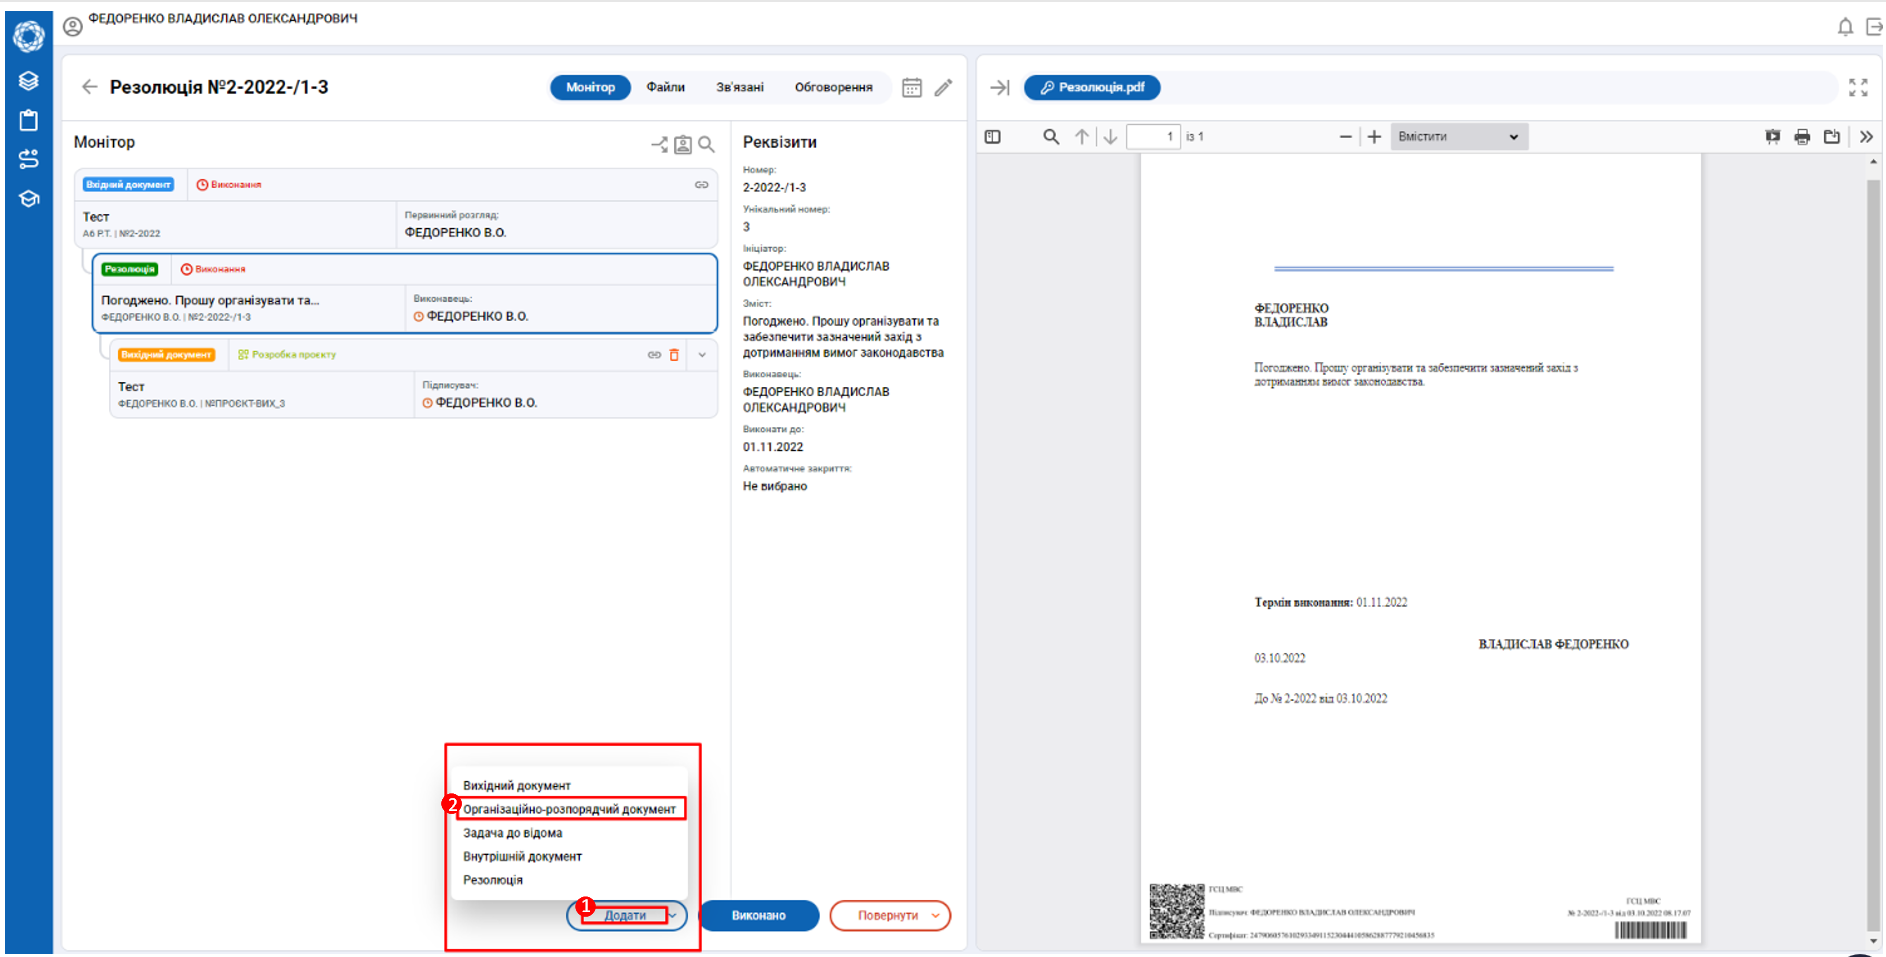
\includegraphics[width=\textwidth]{img/5.5.1.1.png}}
\caption{Рис. 5.5.1.1. Створення проєкта організаційно-розпорядчого документа}
\end{figure}

Система виведе на екран нову форму → показано на Рисунку 5.5.1.2;
--- у графі «Вид документа» розгорніть перелік → виберіть необхідний
документ → на Рисунку 5.5.1.2 прикладом обрано Доручення.

\begin{figure}[!htbp]
\centerline{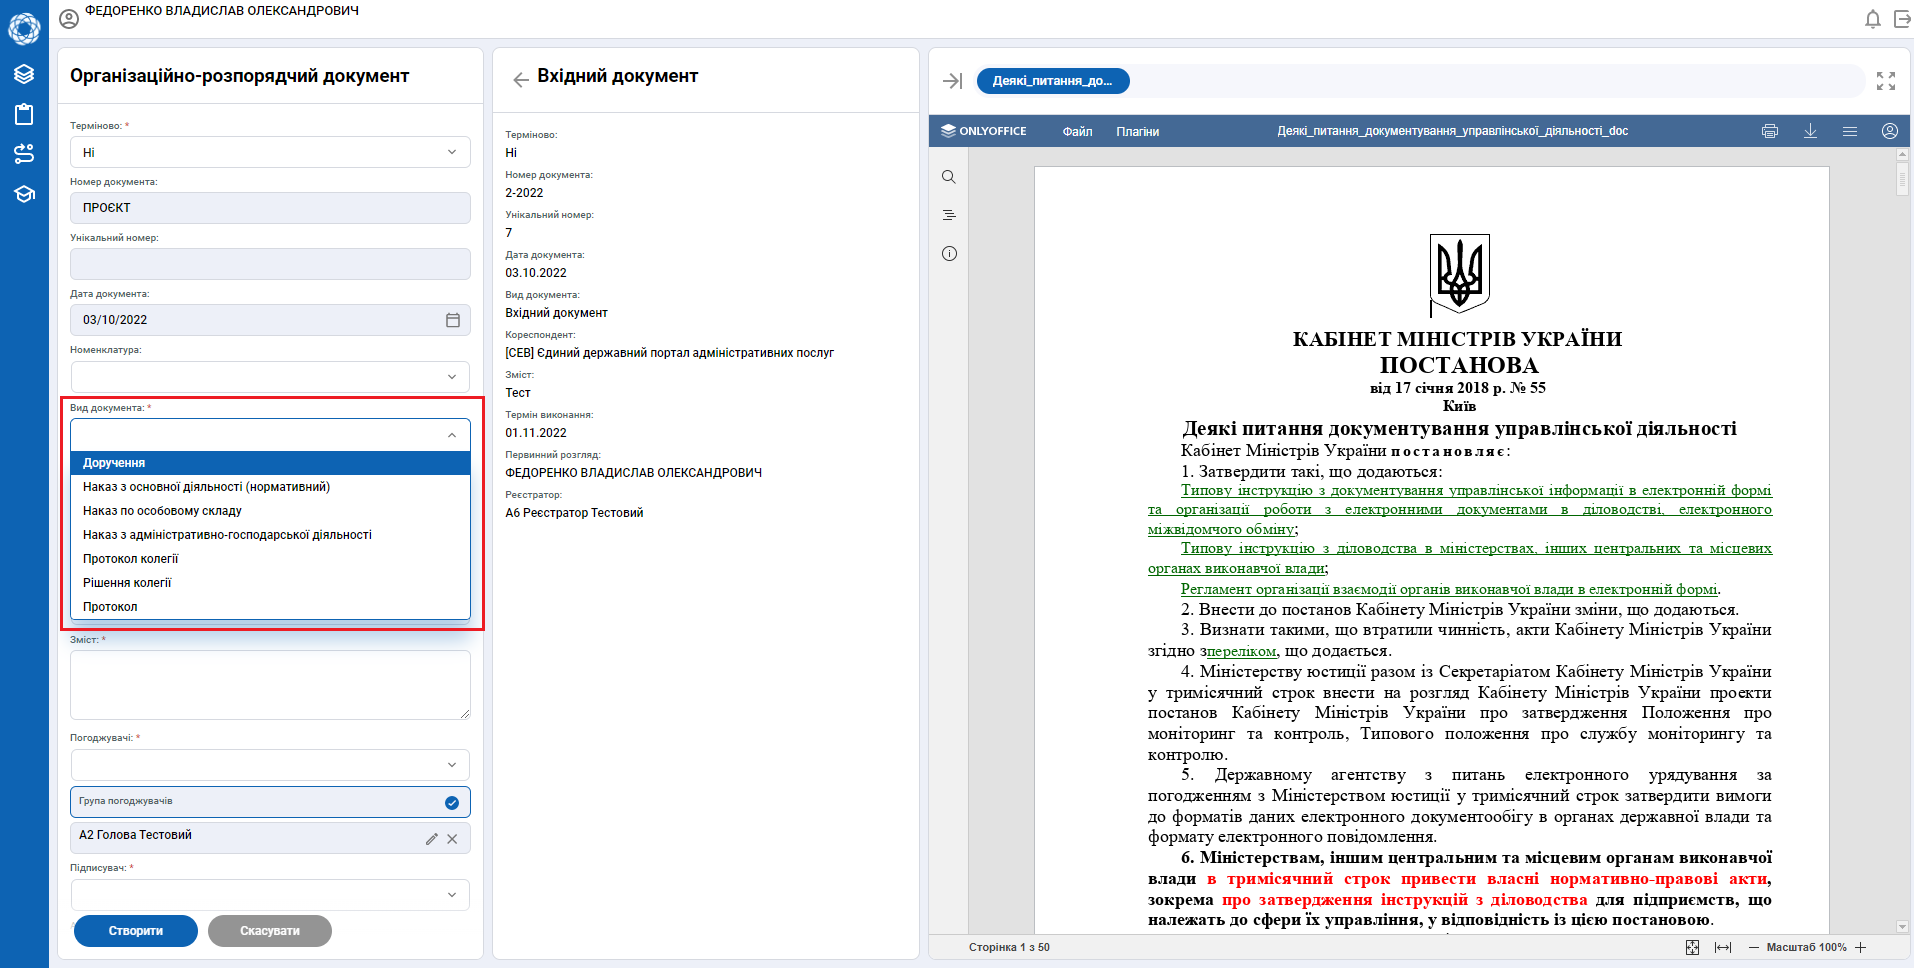
\includegraphics[width=\textwidth]{img/5.5.1.2.png}}
\caption{Рис. 5.5.1.2. Вибір виду документа}
\end{figure}

--- облаcть введення даних → позначена червоною рамкою на Рисунку 5.5.1.3
являє собою РМК → заповніть її (поля відмічені \circled{$\ast$} – обов’язкові для
заповнення).

\begin{figure}[!htbp]
\centerline{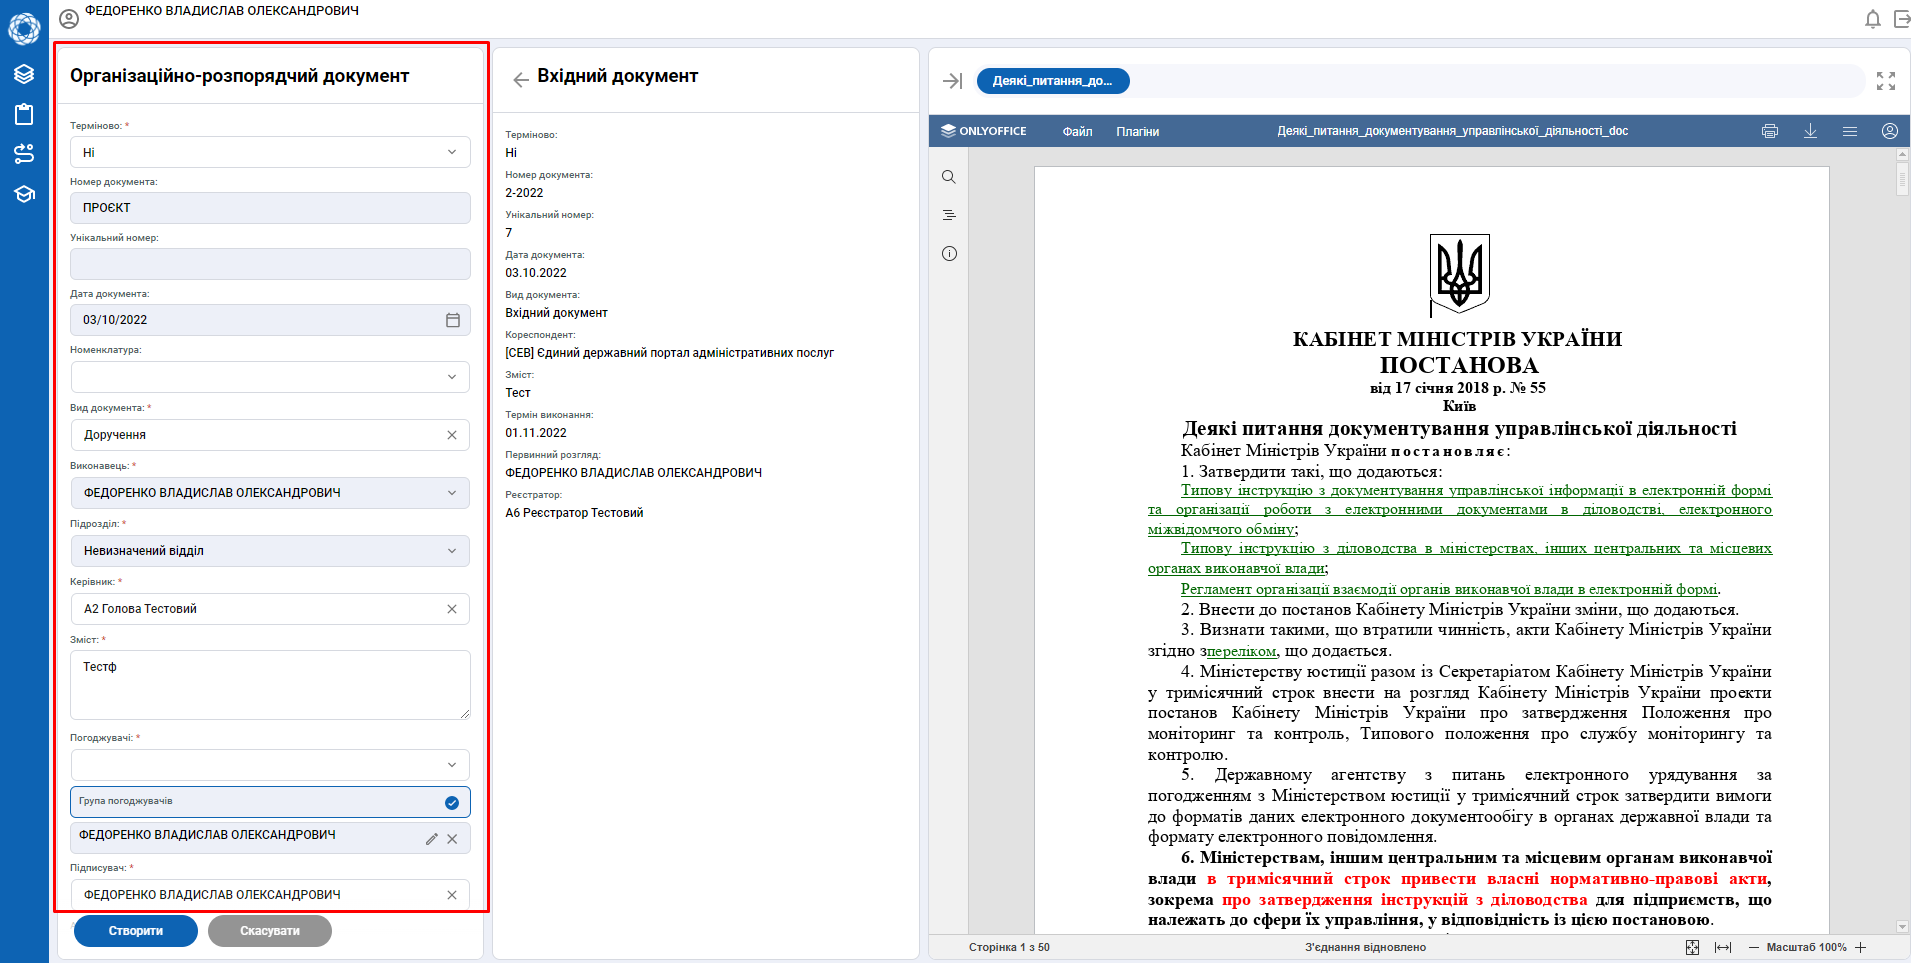
\includegraphics[width=\textwidth]{img/5.5.1.3.png}}
\caption{Рис. 5.5.1.3. Область введення даних РМК}
\end{figure}

--- оберіть «Тип шаблону» → в даному випадку Доручення → позначено
червоною рамкою на Рисунку 5.5.1.4;

\begin{figure}[!htbp]
\centerline{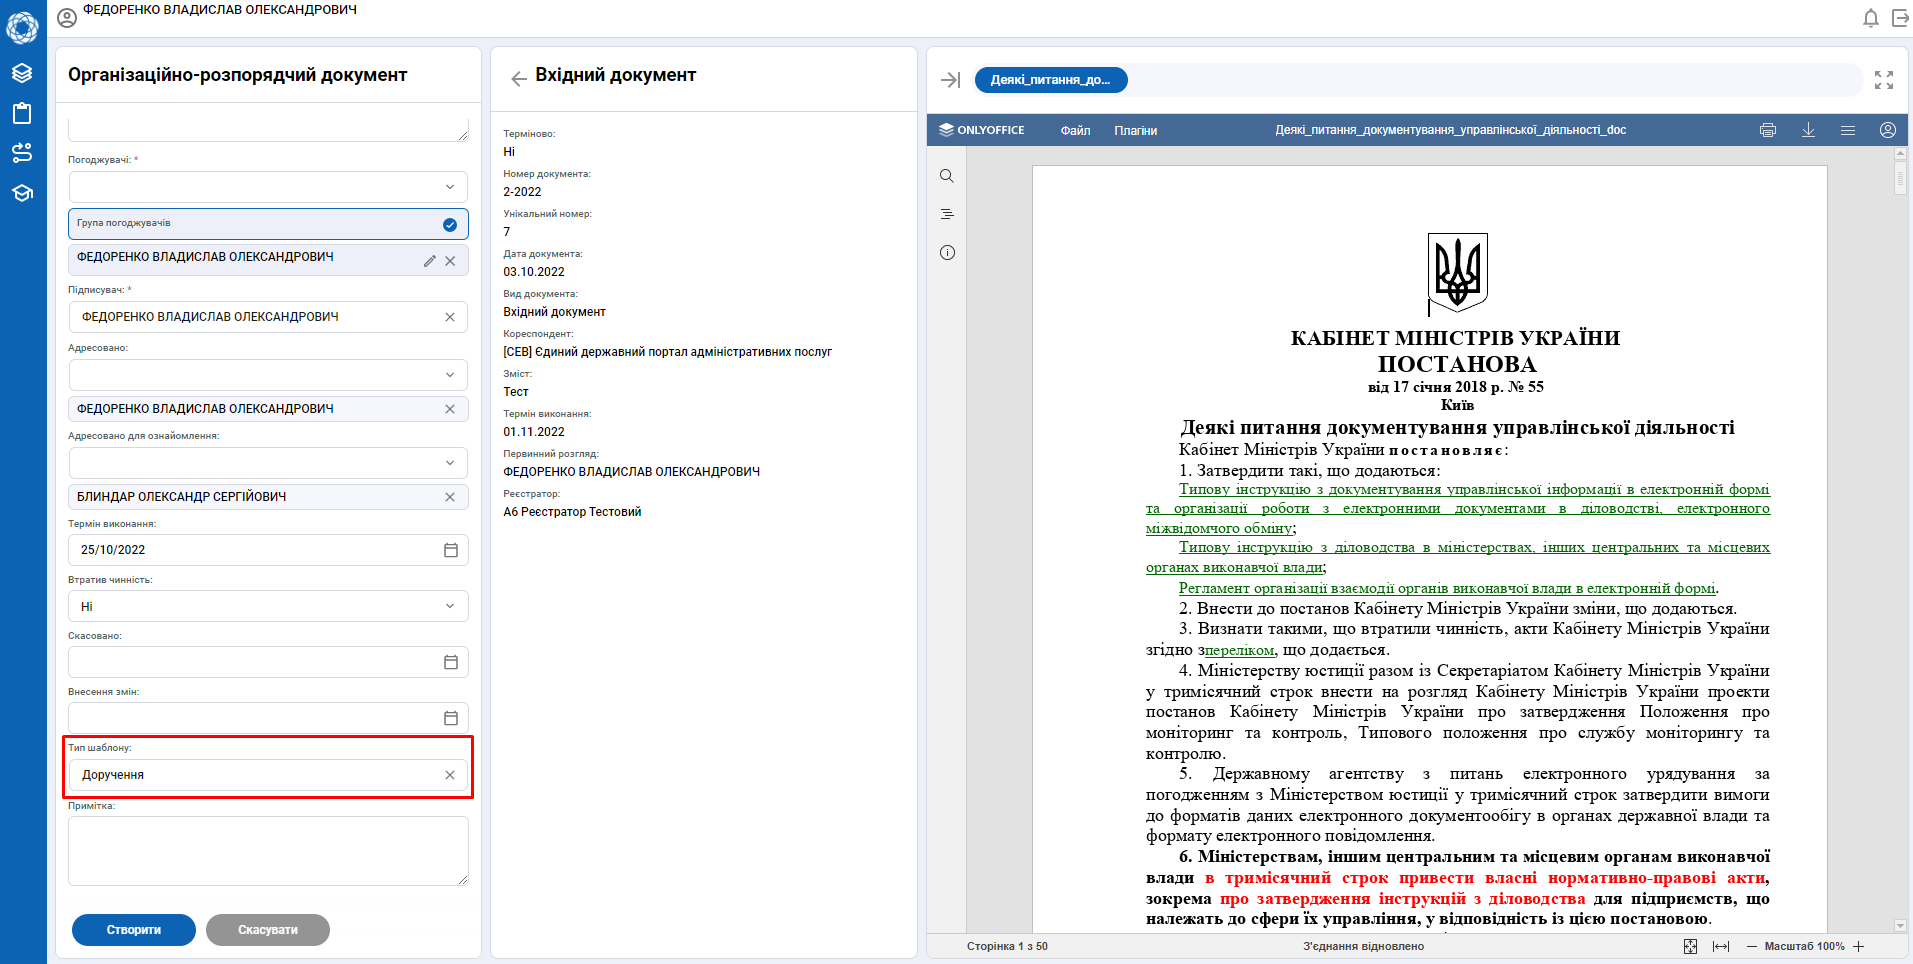
\includegraphics[width=\textwidth]{img/5.5.1.4.png}}
\caption{Рис. 5.5.1.4. Вибір типу шаблону}
\end{figure}

--- натисніть активний елемент «Створити» → позначено червоною рамкою на Рисунку 5.5.1.5;
--- документ успішно створено.

\begin{figure}[!htbp]
\centerline{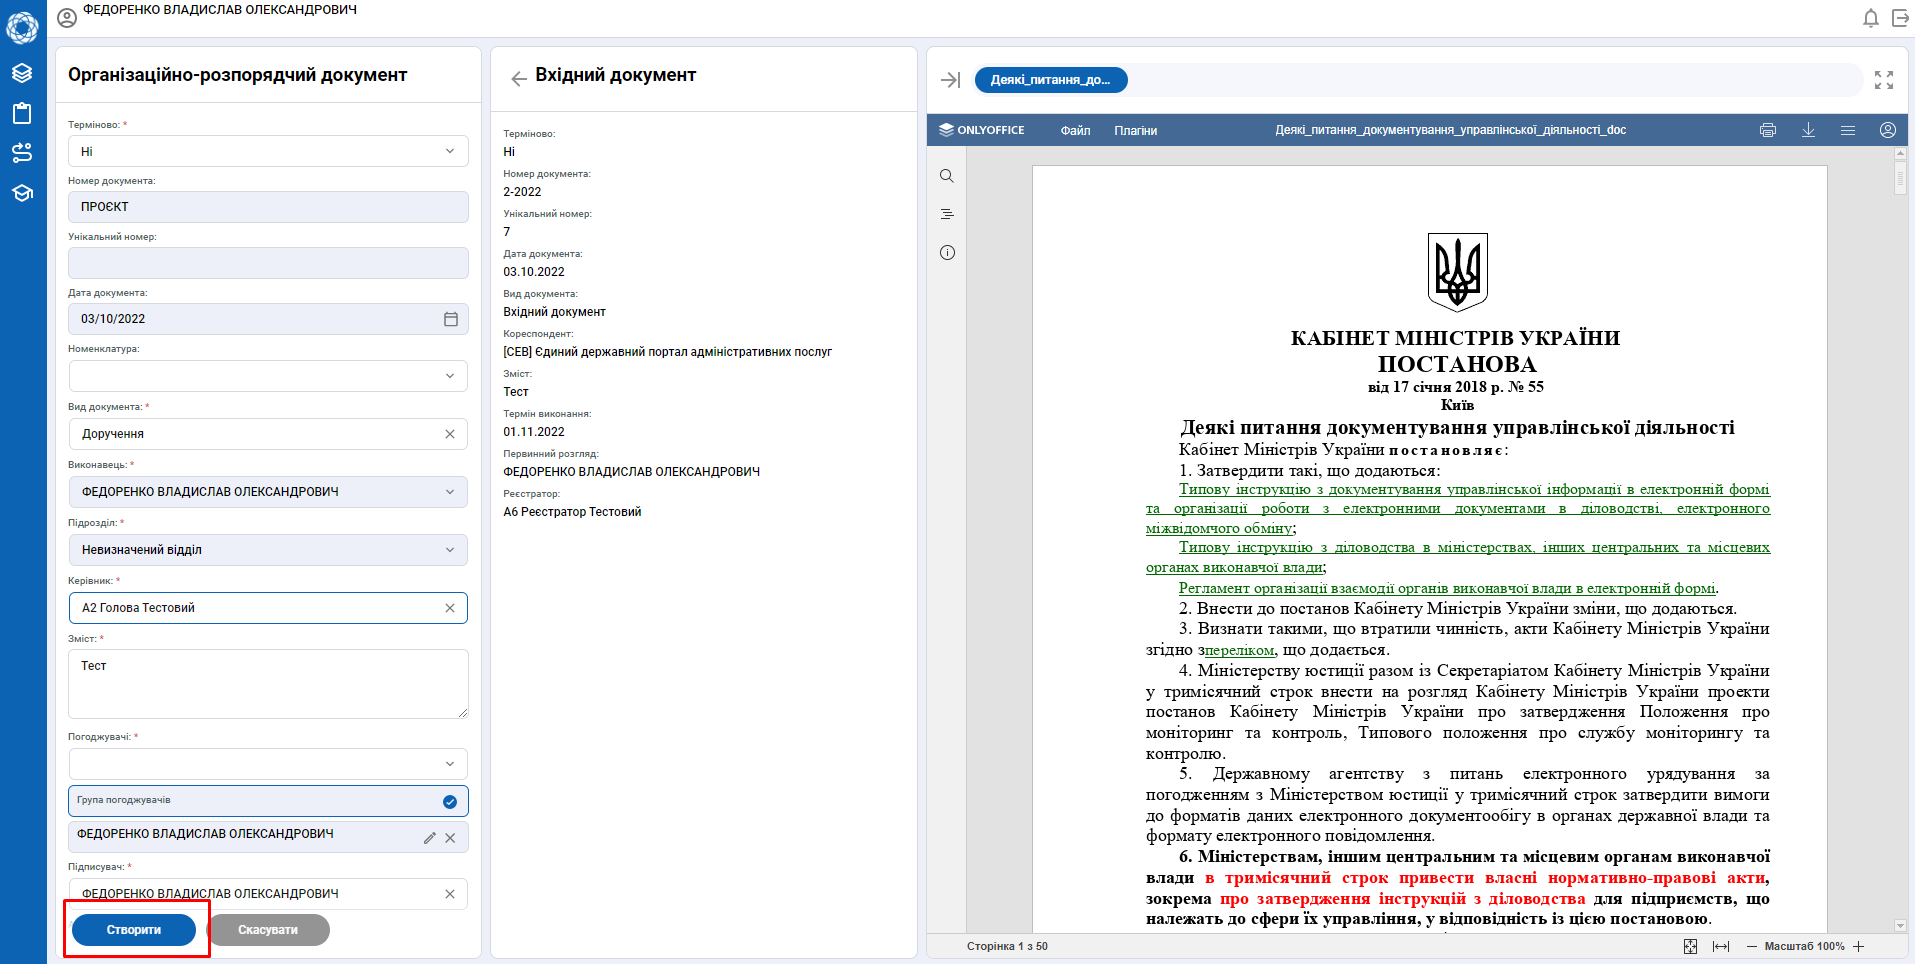
\includegraphics[width=\textwidth]{img/5.5.1.5.png}}
\caption{Рис. 5.5.1.5. Закінчення створення проєкта організаційно-розпорядчого документа}
\end{figure}

\subsection{Редагування \\ організаційно-розпорядчого документа}

Для Редагування організаційно-розпорядчого документа:
--- натисніть піктограму «Редагування» → позначено цифрою \circled{1} на Рисунку 5.5.2.1.

\begin{figure}[!htbp]
\centerline{\includegraphics[width=\textwidth]{img/5.5.2.1.png}}
\caption{Рис. 5.5.2.1. Активація меню редагування організаційно-розпорядчого документа}
\end{figure}

Меню «Редагування» дає можливість користувачу:
\circled{1} --- внести зміни в поля РМК;
\circled{2} --- додати матеріали;
\circled{3} --- відсканувати додаткові матеріали;
\circled{4} --- відредагувати/ заповнити шаблон/ доданий файл, якщо він у форматі *.docx.
--- умовні позначення меню редагування (відмічені цифрами) представлені на Рисунку 5.5.2.2.

\begin{figure}[!htbp]
\centerline{\includegraphics[width=\textwidth]{img/5.5.2.2.png}}
\caption{Рис. 5.5.2.2. Умовні позначення меню редагування}
\end{figure}

для редагування доданого шаблону/ доданого файлу → внесіть відповідні зміни в проєкт організаційно-розпорядчого документа;
--- після внесення змін → натисніть піктограму «Зберегти» → позначено цифрою \circled{1} на Рисунку 5.5.2.3;
--- для підтвердження змін → натисніть активний елемент «Змінити» → позначено цифрою \circled{2} на Рисунку 5.5.2.3.

\begin{figure}[!htbp]
\centerline{\includegraphics[width=\textwidth]{img/5.5.2.3.png}}
\caption{Рис. 5.5.2.3. Підтвердження змін в проєкті організаціно-розпорядчого документа}
\end{figure}

\subsection{Видалення проєкта \\ організаційно-розпорядчого документа}

Для Видалення проєкта організаційно-розпорядчого документа:
--- натисніть піктограму «Видалити» → позначено цифрою \circled{1} на Рисунку 5.5.3.1.

\begin{figure}[!htbp]
\centerline{\includegraphics[width=\textwidth]{img/5.5.3.1.png}}
\caption{Рис. 5.5.3.1. Видалення проєкта організаційно-розпорядчого документа}
\end{figure}

у підсумку процеси створення/ редагування проєкта організаційнорозпорядчого документа
закінчуються переходом на стадію «Погодження» (згідно списку погодження, що було
визначено в процесі заповнення РМК).
--- для погодження документа → натисніть активний елемент «На погодження» → позначений
цифрою \circled{1} на Рисунку 5.5.3.2.

\begin{figure}[!htbp]
\centerline{\includegraphics[width=\textwidth]{img/5.5.3.2.png}}
\caption{Рис. 5.5.3.2. Погодження документа}
\end{figure}

\section{Пошук документів}

Для Пошуку документів:
--- відкрийте панель пошуку документів на Робочому столі → натисніть
піктограму «Пошук» → позначена цифрою \circled{1} на Рисунку 5.6.1;

\begin{figure}[!htbp]
\centerline{\includegraphics[width=\textwidth]{img/5.6.1.png}}
\caption{Рис. 5.6.1. Панель пошуку на Робочому столі}
\end{figure}

для пошуку документа → виберіть параметри пошуку → область вибору позначена цифрою \circled{1} на Рисунку 5.6.2;
--- натисніть активний елемент «Шукати» → позначено цифрою \circled{2} на Рисунку 5.6.2;
--- примітка: за замовчуванням здійснюється пошук «По всіх документах».

\begin{figure}[!htbp]
\centerline{\includegraphics[width=\textwidth]{img/5.6.2.png}}
\caption{Рис. 5.6.2. Пошук документа за параметрами}
\end{figure}

--- примітка 2: якщо не вказати параметри пошуку → відображаються всі
доступні користувачеві документи. 

\section{Погодження}

\subsection{Погодження проєкту документа}

Для Погодження проєкта документа:
--- погоджувачу необхідно натиснути активний елемент «Погодити» →
позначено цифрою 1 на Рисунку 5.6.1.

\begin{figure}[!htbp]
\centerline{\includegraphics[width=\textwidth]{img/5.7.1.1.png}}
\caption{Рис. 5.7.1.1. Погодження проєкту документа}
\end{figure}

\subsection{Редагування проєкту документа}

Погоджувач має можливість вносити Зміни до проєкту документа:
--- для внесення змін → натисніть піктограму «Редагувати» → позначено
цифрою \circled{1} на Рисунку 5.7.1.1.

\begin{figure}[!htbp]
\centerline{\includegraphics[width=\textwidth]{img/5.7.1.1.png}}
\caption{Рис. 5.7.1.1. Погодження проєкту документа}
\end{figure}

внесіть зміни до проєкту документа → область позначена цифрою \circled{1} на Рисунку 5.7.1.2

\begin{figure}[!htbp]
\centerline{\includegraphics[width=\textwidth]{img/5.7.1.2.png}}
\caption{Рис. 5.7.1.2. Область для внесення змін погоджувачем}
\end{figure}

після внесення необхідних змін натисніть піктограму «Зберегти» → позначено цифрою \circled{1} на Рисунку 5.7.1.3;
--- за необхідності, скористайтеся можливістю прикріпити додаткові файли → область позначена цифрою \circled{2} на Рисунку 5.7.1.3.

\begin{figure}[!htbp]
\centerline{\includegraphics[width=\textwidth]{img/5.7.1.3.png}}
\caption{Рис. 5.7.1.3. }
\end{figure}

Система дозволяє додавати або змінювати Порядок погоджувачів. Для додавання
Нового погоджувача:
--- внесіть прізвище погоджувача у поле «Погоджувачі» РМК → позначено цифрою \circled{1} на Рисунку 5.7.1.4;
--- натисніть «Підтвердити» → позначено цифрою \circled{2} на Рисунку 5.7.1.4.

\begin{figure}[!htbp]
\centerline{\includegraphics[width=\textwidth]{img/5.7.1.4.png}}
\caption{Рис. 5.7.1.4. Додавання нового погоджувача}
\end{figure}

Для додавання Групи погоджувачів (паралельного погодження):
--- внесіть прізвища всіх погоджувачів у поле «Група погоджувачів» РМК → позначено цифрою \circled{1} на Рисунку 5.7.1.5;
--- натисніть «Підтвердити» → позначено цифрою \circled{2} на Рисунку 5.7.1.5.

\begin{figure}[!htbp]
\centerline{\includegraphics[width=\textwidth]{img/5.7.1.5.png}}
\caption{Рис. 5.7.1.5. Додавання групи погоджувачів}
\end{figure}

Для Зміни порядку погоджувачів/ групи погоджувачів:
--- наведіть курсор миші на прізвище погоджувача/ групу погоджувачів →
натисніть праву кнопку миші та перетягніть погоджувача на потрібну
позицію в списку погоджувачів.
Для Редагування погоджувачів/ груп погоджувачів:
--- натисніть піктограму → позначено цифрою \circled{1} на Рисунку 5.7.1.6;
--- внесіть відповідні зміни → цифрами на Рисунку 5.7.1.6 позначено:
\circled{2} --- додавання погоджувачів;
\circled{3} --- видалення погоджувачів та зміна порядку погодження;
--- натисніть «Підтвердити» → позначено цифрою \circled{4} на Рисунку 5.7.1.6. 

\begin{figure}[!htbp]
\centerline{\includegraphics[width=\textwidth]{img/5.7.1.6.png}}
\caption{Рис. 5.7.1.6. Редагування погоджувачів/ груп погоджувачів}
\end{figure}

для збереження змін → натисніть активний елемент «Змінити» → позначено
червоною рамкою на Рисунку 5.7.1.7

\begin{figure}[!htbp]
\centerline{\includegraphics[width=\textwidth]{img/5.7.1.7.png}}
\caption{Рис. 5.7.1.7. Збереження змін у документі}
\end{figure}

Щоб визначити іншу версію документа, як Основну:
--- натисніть вкладку «Файли» → позначено цифрою \circled{1} на Рисунку 5.7.1.8;
--- оберіть необхідну версію (на Рисунку 5.7.1.8 підкреслена червоним);
--- натисніть піктограму «Змінити» → позначено цифрою \circleld{2} на Рисунку 5.7.1.8

\begin{figure}[!htbp]
\centerline{\includegraphics[width=\textwidth]{img/5.7.1.8.png}}
\caption{Рис. 5.7.1.8. Визначення основної версії документа}
\end{figure}

\subsection{Повернення проєкта документа}

Для Повернення проєкта документа автору на стадію розробки проєкта:
--- натисніть активний елемент «Повернути» → позначено цифрою \circled{1} на Рисунку 5.7.2.1;
--- виберіть пункт «На розробку проєкта» → позначено цифрою \circled{2} на Рисунку 5.7.2.1.

\begin{figure}[!htbp]
\centerline{\includegraphics[width=\textwidth]{img/5.7.2.1.png}}
\caption{Рис. 5.7.2.1. Повернення документа на стадію розробки проєкта}
\end{figure}

Обов’язково вкажіть обґрунтовану причину повернення документа →
позначено цифрою 1 на Рисунку 5.7.2.2;
--- натисніть елемент, позначений цифрою \circled{2} на Рисунку 5.7.2.2.

\begin{figure}[!htbp]
\centerline{\includegraphics[width=\textwidth]{img/5.7.2.2.png}}
\caption{Рис. 5.7.2.2. Причина повернення документа}
\end{figure}

\section{Підписання}

\subsection{Підписання проєкту документа}

Для Підписання проєкту документа підписувачу необхідно:
--- натиснути активний елемент «Підписати» → позначено цифрою \circled{1} на
Рисунку 5.8.1.

\begin{figure}[!htbp]
\centerline{\includegraphics[width=\textwidth]{img/5.8.1.png}}
\caption{Рис. 5.8.1. Підписання проєкту документа}
\end{figure}

\subsection{Редагування проєкту документа}

У разі наявності зауважень - Підписувач має можливість вносити Зміни до основного документа:
--- для внесення змін до основного документа → замініть його на .docx версію (див. Рисунок 5.8.1.1):
--- натисніть вкладку «Файли» → позначено цифрою \circled{1};
--- оберіть необхідну версію → натисніть «Змінити» → позначено цифрою \circled{2}.

\begin{figure}[!htbp]
\centerline{\includegraphics[width=\textwidth]{img/5.8.1.1.png}}
\caption{Рис. 5.8.1.1. Заміна документа на .docx версію}
\end{figure}

Для продовження Редагування:
--- повернутися до вкладки «Монітор» → позначено цифрою \circled{1} на Рисунку 5.8.1.2
--- натиснути піктограму «Редагування» → позначено цифрою \circled{2} на Рисунку 5.8.1.2 

\begin{figure}[!htbp]
\centerline{\includegraphics[width=\textwidth]{img/5.8.1.2.png}}
\caption{Рис. 5.8.1.2. Повернення до процесу редагування}
\end{figure}

Внести зміни до проєкту документа → область позначена цифрою \circled{1} на Рисунку 5.8.1.3.

\begin{figure}[!htbp]
\centerline{\includegraphics[width=\textwidth]{img/5.8.1.3.png}}
\caption{Рис. 5.8.1.3. Внесення змін у документ}
\end{figure}

Після внесення змін → натисніть піктограму «Зберегти» (виділена
червоною рамкою) у верхній правій частині вікна OnlyOffice на Рисунку Рис.5.8.1.4.

\begin{figure}[!htbp]
\centerline{\includegraphics[width=\textwidth]{img/5.8.1.4.png}}
\caption{Рис. 5.8.1.4. Збереження змін, внесених у документ}
\end{figure}

За необхідності – прикріпіть додаткові файли (див. Рисунок 5.8.1.5).

\begin{figure}[!htbp]
\centerline{\includegraphics[width=\textwidth]{img/5.8.1.5.png}}
\caption{Рис. 5.8.1.5. Область прикріплення додаткових файлів}
\end{figure}

--- Для збереження оновленого документа → натисніть активний елемент
«Змінити» → позначено червоною рамкою на Рисунку 5.8.1.6.

\begin{figure}[!htbp]
\centerline{\includegraphics[width=\textwidth]{img/5.8.1.6.png}}
\caption{Рис. 5.8.1.6. Збереження оновленого документа}
\end{figure}

\subsection{Повернення проєкта документа}

Для повернення проєкту документа на розробку проєкта/на погодження:
--- натисніть активний елемент «Повернути» → позначено цифрою \circled{1} на Рисунку 5.8.2.1;
--- виберіть пункт «На розробку проєкта»/ «На погодження» → позначено цифрою \circled{2} на Рисунку 5.8.2.1.

\begin{figure}[!htbp]
\centerline{\includegraphics[width=\textwidth]{img/5.8.2.1.png}}
\caption{Рис. 5.8.2.1. Повернення документа}
\end{figure}

Вкажіть обґрунтовану причину повернення → позначено цифрою 1 на
Рисунку 5.8.2.2 → та натисніть кнопку 2 (див. виділені червоним елементи
на Рисунку 5.8.2.2)

\begin{figure}[!htbp]
\centerline{\includegraphics[width=\textwidth]{img/5.8.2.2.png}}
\caption{Рис. 5.8.2.2. Причина повернення документа}
\end{figure}

\section{Групування}

Всі виконавці по документу виконали свої завдання.
2. Після виконання завдань – натиснули кнопку «Виконано».
3. Документ переходить на стадію «Групування».
4. Реєстратор відправляє документ на «Зберігання».

Щоб відправити документ на Зберігання:
--- Реєстратор натискає на активний елемент «На зберігання» → позначено цифрою \circled{1} на Рисунку 5.9.1;
--- або реєстратор повертає документ → натисніть активний елемент «Повернути» → позначено цифрою \circled{2} на Рисунку 5.9.1
--- обрати пункт «На попередню стадію» → позначено цифрою \circled{3} на Рисунку 5.9.1.

\begin{figure}[!htbp]
\centerline{\includegraphics[width=\textwidth]{img/5.9.1.png}}
\caption{Рис. 5.9.1. Cтадія Групування}
\end{figure}

\section{Проєкт відправки}

Після накладення підпису вихідний документ переходить на стадію «Проєкт відправки».
Для відправлення документа Реєстратору необхідно:
--- натиснути активний елемент «На відправку» → позначено цифрою \circled{1} на Рисунку 5.10.1

\begin{figure}[!htbp]
\centerline{\includegraphics[width=\textwidth]{img/5.10.1.png}}
\caption{Рис. 5.10.1. }
\end{figure}

Перейдіть у процес відправки – позначено цифрою \circled{1} на Рисунку 5.10.2.

\begin{figure}[!htbp]
\centerline{\includegraphics[width=\textwidth]{img/5.10.2.png}}
\caption{Рис. 5.10.2. }
\end{figure}

Натисніть активний елемент «Відправити» → позначено цифрою \circled{1} на Рисунку 5.10.3.

\begin{figure}[!htbp]
\centerline{\includegraphics[width=\textwidth]{img/5.10.3.png}}
\caption{Рис. 5.10.3. }
\end{figure}

Щоб змінити:
1) тип відправки (СЕВ, Еmail, поштою тощо);
2) змінити кореспондента/ додати кореспондентів необхідно
→ натиснути піктограму «Редагування» → позначено цифрою \circled{1} на Рисунку 5.10.4.

\begin{figure}[!htbp]
\centerline{\includegraphics[width=\textwidth]{img/5.10.4.png}}
\caption{Рис. 5.10.4. }
\end{figure}

В реквізитах документа в полі вибраного кореспондента → оберіть тип
відправки → позначено цифрою \circled{2} на Рисунку 5.10.5;
--- Натисніть кнопку вибору → позначено цифрою \circled{1} на Рисунку 5.10.5.

\begin{figure}[!htbp]
\centerline{\includegraphics[width=\textwidth]{img/5.10.5.png}}
\caption{Рис. 5.10.5. }
\end{figure}

Щоб додати необхідні матеріали → натисніть область, позначену цифрою
\circled{1} на Рисунку 5.10.6 або перетягніть підготовлений документ в це поле.
--- коли всі зміни будуть внесені → натисніть активний елемент «Змінити» →
позначено цифрою \circled{2} на Рисунку 5.10.6.

\begin{figure}[!htbp]
\centerline{\includegraphics[width=\textwidth]{img/5.10.6.png}}
\caption{Рис. 5.10.6. }
\end{figure}

Натисніть активний елемент «На відправку» → позначено цифрою \circled{1} на Рисунку 5.10.7.

\begin{figure}[!htbp]
\centerline{\includegraphics[width=\textwidth]{img/5.10.7.png}}
\caption{Рис. 5.10.7. }
\end{figure}

\newpage
Наступні етапи повторюють процеси прокоментовані та відображені на Рисунках
5.10.2 та 5.10.3:

--- Перейдіть у процес відправки – позначено цифрою \circled{1} на Рисунку 5.10.8.

\begin{figure}[!htbp]
\centerline{\includegraphics[width=\textwidth]{img/5.10.8.png}}
\caption{Рис. 5.10.8. Процес відправки}
\end{figure}

Натисніть активний елемент «Відправити» → позначено цифрою 1 на Рисунку 5.10.9

\begin{figure}[!htbp]
\centerline{\includegraphics[width=\textwidth]{img/5.10.9.png}}
\caption{Рис. 5.10.9. Відправлення документа.}
\end{figure}

